\documentclass[a4paper,12pt,twoside,openright]{report}
% to make lins space single 
%\usepackage{setspace}
%% to remove page numbers from blanck pages 
\usepackage{emptypage} 
% to adjust margins 
\usepackage[margin=1in,left=35.4mm]{geometry} 
% to use times new roman font 
\usepackage{times} 
% to use math library 
\usepackage{amsmath, amsthm, amssymb,mathrsfs}  
\usepackage{comment}
\usepackage{booktabs}
\usepackage{longtable}
\usepackage{ragged2e}
\usepackage{changepage}
\usepackage{siunitx}
\usepackage{tikz}
\usepackage[american]{circuitikz}
\usetikzlibrary{shapes, arrows.meta, positioning, calc, backgrounds}
%----------------------------------
% to add list of abbriviation and symbols 
%\usepackage[intoc]{nomencl}
%\renewcommand{\nomname}{List of Abbreviations}
%\makenomenclature
%%%https://tex.stackexchange.com/questions/86666/how-to-create-both-list-of-abbreviations-and-list-of-nomenclature-using-nomencl/87223
%% This removes the main title:
%\renewcommand{\nomname}{}
%% this modifies item separation:
%\setlength{\nomitemsep}{8pt}
%% this part defines the groups:
%\usepackage{etoolbox}
%\renewcommand\nomgroup[1]{%
%	\item[\Large\bfseries
%	\ifstrequal{#1}{A}{List of Abbreviations}{%
%	\ifstrequal{#1}{S}{List of Symbols}{}}%
%	]\vspace{10pt}} % this is to add vertical space between the groups.
%----------------------------------------------
%\numberwithin{figure}{chapter}
%\numberwithin{equation}{chapter}  % to number with chapter
\usepackage{graphicx} 
% to make captions bold
\usepackage[labelfont=bf,font=bf,justification=centering]{caption} %{labelsep=space}  
\usepackage{caption}
\usepackage{subcaption}
\usepackage{float} % to adjust some figures positions with control letter H

%\graphicspath{{./Chapters/Introduction/Pictures/}}
%table packages and text wraping 
%https://stackoverflow.com/questions/790932/how-to-wrap-text-in-latex-tables
\usepackage{tabularx}
\usepackage{array}
\newcolumntype{L}{>{\centering\arraybackslash}m{5cm}}
\usepackage{multirow}
% hyperlinks within document 
\usepackage[hidelinks]{hyperref} 
% references 
%\usepackage{cite} 
\usepackage[backend=bibtex,style=numeric,sorting=none,citestyle=numeric-comp]{biblatex}
% ------- to remove all italics in cittion names
\makeatletter
\renewrobustcmd*{\mkbibemph}{}
\protected\long\def\blx@imc@mkbibemph#1{#1}
\makeatother
% -------
\DeclareFieldFormat{labelnumberwidth}{#1\adddot} % to make list of references DOTs instead of [ ]
\addbibresource{BIB_AD.bib} 
%----------------------------------------------%
%https://tex.stackexchange.com/questions/246744/cant-print-bibliography/246745
%----------------------------------------------%
\usepackage[titletoc]{appendix}
% to import pdfs 
\usepackage{pdfpages}
% to add euro symbole  
\usepackage{eurosym} 
% to capitiliza first letter. 
\usepackage{titlecaps} 
\Addlcwords{before and after}  % excluded words 
% https://tex.stackexchange.com/questions/335990/is-there-a-command-to-make-first-letter-upper-case  
% 
\setlength{\parindent}{12pt}   % first-line indent
\setlength{\parskip}{0.5em}    % vertical space between paragraphs
% to adjust spacing before and after toc, lof and lot 
%https://tex.stackexchange.com/questions/62125/how-to-remove-top-margin-above-tableofcontents 
\usepackage{tocloft}
\setlength{\cftbeforetoctitleskip}{0pt}
\setlength{\cftaftertoctitleskip}{36pt}
\setlength{\cftbeforeloftitleskip}{0pt}
\setlength{\cftafterloftitleskip}{36pt}
\setlength{\cftbeforelottitleskip}{0pt}
\setlength{\cftafterlottitleskip}{36pt}
\renewcommand \cftchapdotsep{4.5}
%to change the default naming of toc,lof and lot
\renewcommand{\contentsname}{\hspace{3.5cm} Table of Contents}
\renewcommand{\cftchappresnum}{CHAPTER } % CHAPTER before number in ToC
\newlength{\mylen} % a scratch length
\settowidth{\mylen}{\bfseries\cftchappresnum\cftchapaftersnum} % extra space
\addtolength{\cftchapnumwidth}{\mylen} % add the extra space


\renewcommand{\cftlottitlefont}{\hspace*{\fill}\Huge\bfseries}
\renewcommand{\cftafterlottitle}{\hspace*{\fill}}
\renewcommand{\cftloftitlefont}{\hspace*{\fill}\Huge\bfseries}
\renewcommand{\cftafterloftitle}{\hspace*{\fill}}
\renewcommand{\cftchapaftersnum}{:}
\renewcommand{\cftfigpresnum}{Figure\ }
\renewcommand{\cfttabpresnum}{Table\ }
% set space betwwenfigure word and caption in toc
\newlength{\mylenf}
\settowidth{\mylenf}{\cftfigpresnum}
\setlength{\cftfignumwidth}{\dimexpr\mylenf+2em}
\setlength{\cfttabnumwidth}{\dimexpr\mylenf+2em}
%https://tex.stackexchange.com/questions/20337/adding-word-table-before-each-entry-in-list-of-tables



%%page layout frames 
%\usepackage{showframe} % to show layout frams 
%\renewcommand\ShowFrameLinethickness{0.15pt}
%\renewcommand*\ShowFrameColor{\color{red}}

% to adjust chapter naming spacing 
% https://tex.stackexchange.com/questions/25030/chapter-number-and-chapter-title-in-one-line
% https://tex.stackexchange.com/questions/310205/is-there-a-way-to-center-align-chapter-titles





\usepackage{titlesec}
\usepackage{tocloft}

% Center the chapter titles
\titleformat{\chapter}[display]
{\normalfont\huge\bfseries\filcenter} % Centering the chapter title
{\chaptertitlename\ \thechapter}{20pt}{\Huge}

% Define subsubsubsection
\titleclass{\subsubsubsection}{straight}[\subsubsection]
\newcounter{subsubsubsection}[subsubsection]
\renewcommand\thesubsubsubsection{\thesubsubsection.\arabic{subsubsubsection}}
\titleformat{\subsubsubsection}
{\normalfont\normalsize\itshape}{\thesubsubsubsection}{1em}{}
\titlespacing*{\subsubsubsection}
{0pt}{0.5em}{0.5em}

% Enable subsubsubsection in TOC
\setcounter{secnumdepth}{4}
\setcounter{tocdepth}{4}

% Define subsubsubsection for tocloft with proper spacing
\makeatletter
\newcommand{\l@subsubsubsection}{\@dottedtocline{4}{4.5em}{3.8em}}
\makeatother



% Change chapter title format to centered "Chapter X: Title"
% Define chapter title format in one line and centered
\titleformat{\chapter}[block]
{\normalfont\fontsize{18}{22}\bfseries\centering} % Sets font size to 18pt
{Chapter \thechapter:}{0.5em}{} % Chapter number with colon and space for title
[]

%\titleformat{\chapter}[block]
%{\normalfont\huge\bfseries\centering} % Centered and bold
%{Chapter \thechapter:}{0.5em}{} % Chapter number with colon and space for title
%[]
\titleformat{\section}
{\normalfont\fontsize{16}{20}\bfseries} % Sets font size to 16pt, bold
{\thesection}{1em}{} % Keeps section numbering and spacing




\begin{document}
	%	\singlespacing
	% import cover pages till Acknowledgments
	%
\includepdf[pages={1-4}]{Chapters/FrontPages/CUFEThesisTemplate.pdf} --> To be uncommented in final version
	
	\setcounter{page}{1}
	\pagenumbering{roman}
	%
\includepdf[pages={5-6},pagecommand={}]{Chapters/FrontPages/CUFEThesisTemplate.pdf} --> To be uncommented in final version
	
	\clearpage
	\tableofcontents
	%\addcontentsline{toc}{chapter}{Table of Contents}
	
	\clearpage
	\listoftables
	%\cleardoublepage
	%\phantomsection
	\addcontentsline{toc}{chapter}{List of Tables}
	%\let\cleardoublepage\clearpage
	\clearpage
	\listoffigures
	%\cleardoublepage
	%\phantomsection
	\addcontentsline{toc}{chapter}{List of Figures}
	
	%	\input{Chapters/FrontPages/Nomenclature}
	\clearpage
	%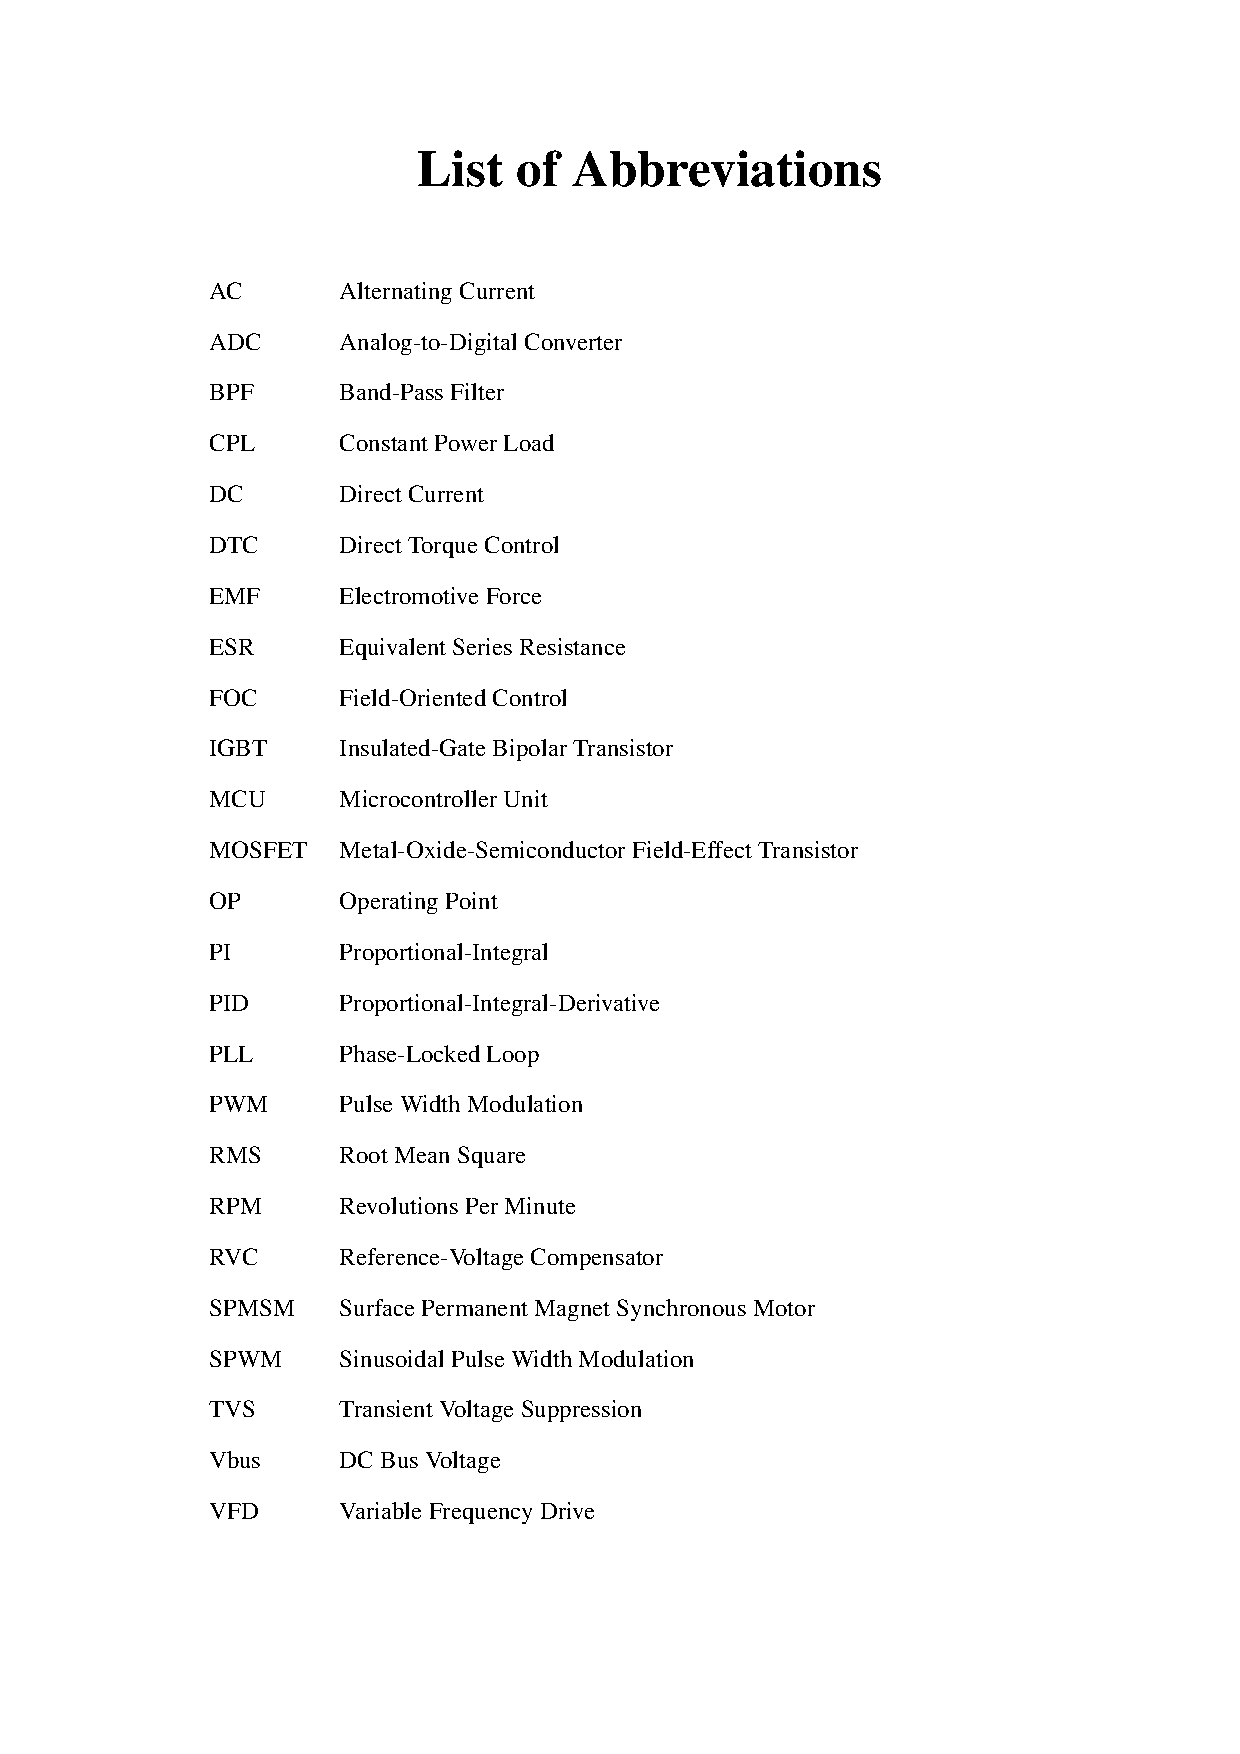
\includepdf[pages={1},pagecommand={\thispagestyle{plain}}]{Chapters/FrontPages/LOA.pdf}
	\addcontentsline{toc}{chapter}{List of Abbreviations}
	
	\clearpage
	%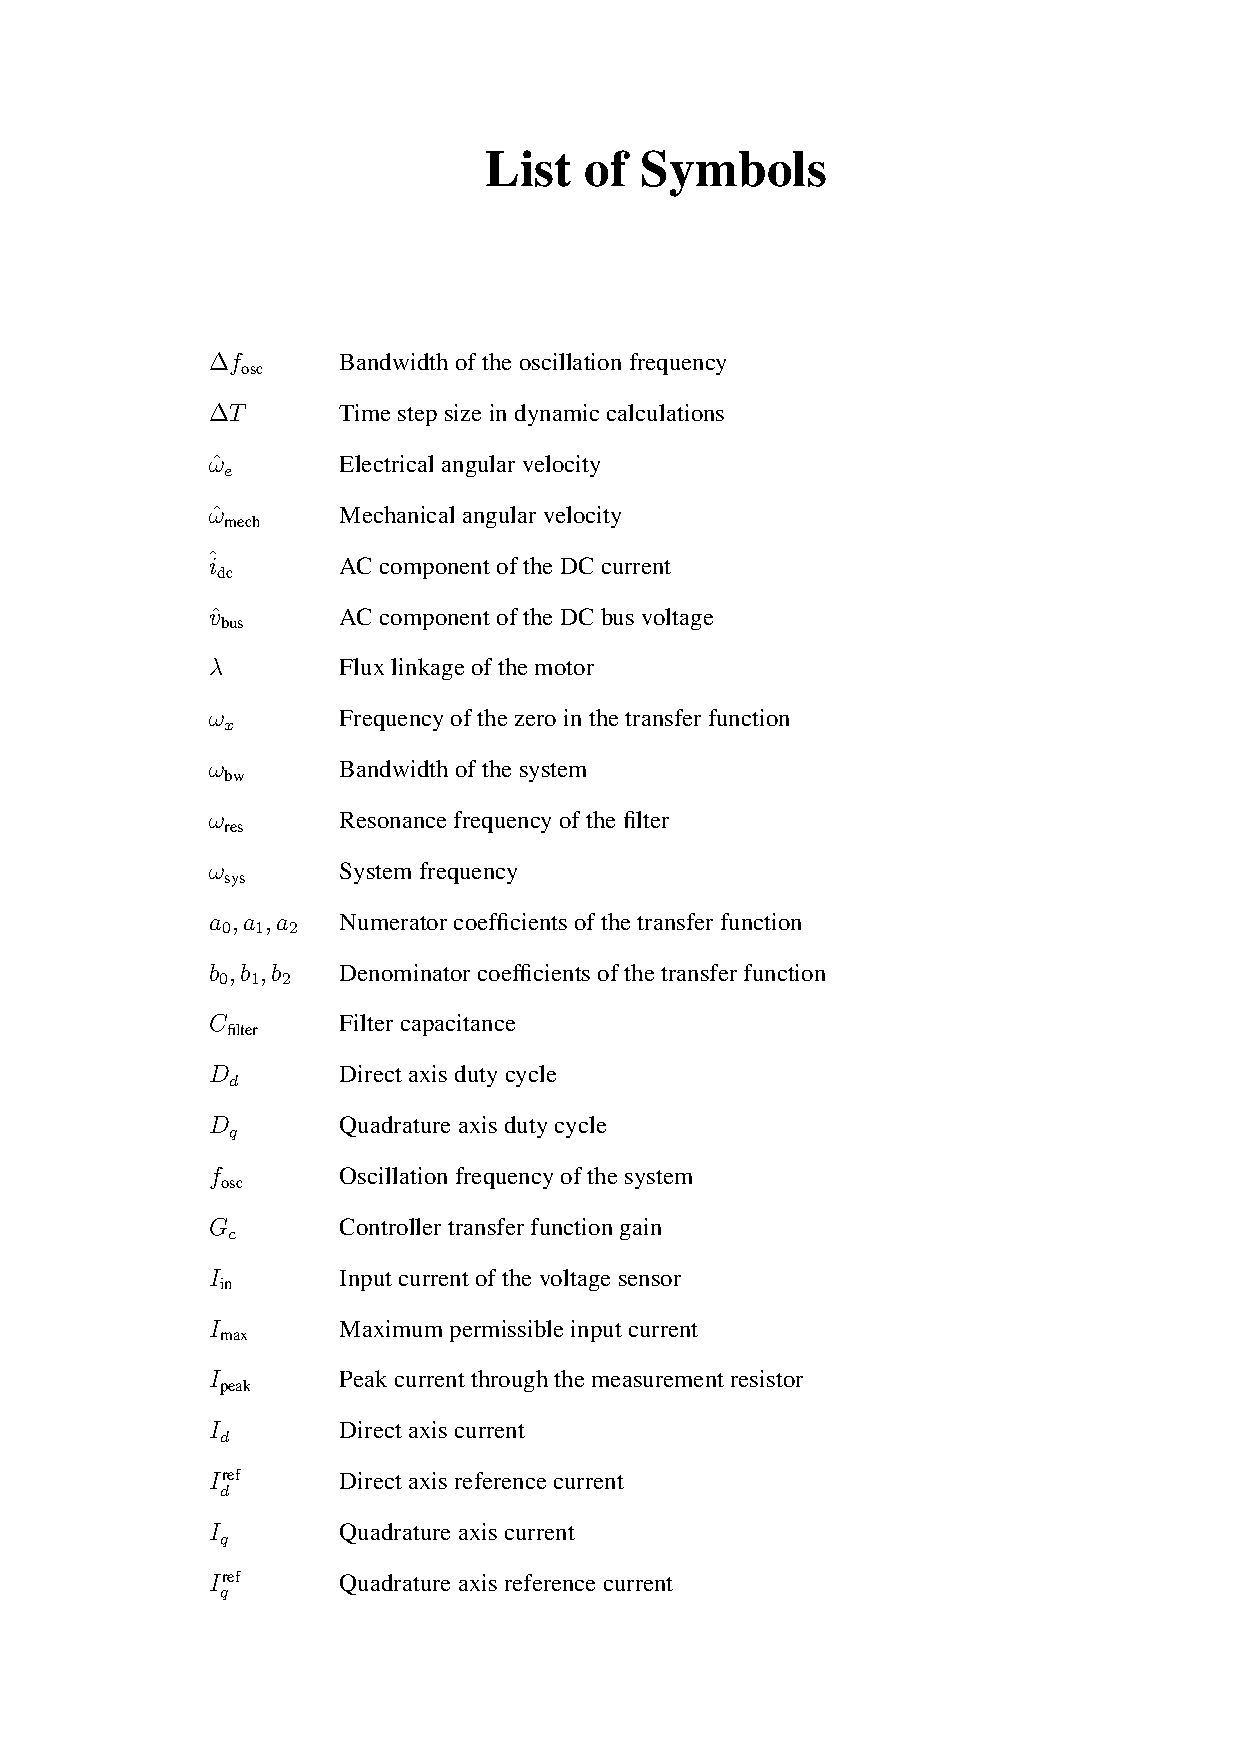
\includepdf[pages={1-2},pagecommand={\thispagestyle{plain}}]{Chapters/FrontPages/LOS.pdf}
	\addcontentsline{toc}{chapter}{List of Symbols}
	% include abstract directly 
	\newpage
	%\chapter*{Abstract}
	% Nomenclature 
%\newpage
%\addcontentsline{toc}{chapter}{Nomenclature}
%\begin{center}
%	\textbf{\large Nomenclature}
%\end{center} 
%You may include a list of alphabetically ordered symbols and abbreviations here.

% Abstract 
\newpage
\addcontentsline{toc}{chapter}{Abstract}
\begin{center}
	\textbf{\large Abstract}
\end{center} 

% =======================
% Abstract (revised)
% =======================
Permanent-magnet synchronous motors (PMSMs) enable efficient, high-density electric drives, but inverter non-linearities (dead time, and device drops) undermine low-speed, sensorless operation by injecting low-order harmonic distortion. This thesis examines three control strategies under that constraint. First, we implemented finite-control-set MPC (FCS–MPC) as a candidate solution. While conceptually simple, its single-vector, variable-frequency actuation yields a voltage shape that interacts unfavorably with the non-linear inverter biases, leading to elevated current THD and fragile low-speed behavior. To avoid variable frequency and reduce the sensitivity to those biases, we then adopted a MMPC that optimizes a continuous average voltage each sample and realizes it via space-vector modulation (SVM), fixing the switching frequency. Finally, we augmented MMPC with a harmonic-extraction (HE) stage that selectively cancels the dominant distortion components in the commanded average voltage to directly target the non-linearity footprint.

A unified simulation campaign compares PI–FOC, FCS–MPC, MMPC, and the proposed MMPC-HE across steady state, low-speed operation, dynamic speed steps (10--50\% rated), load steps (10--100\% rated torque), and parameter variation ($R{+}25\%$, $L{-}25\%$), under both ideal and non-ideal inverter models. Under non-linearities, FCS is unstable at 5\% rated speed and retains high THD at 10\% (e.g., $\sim34\%$ at low load), while PI also struggles at 5\% and shows sizable distortion at 10\% (e.g., $\sim23\%$ at low load). In contrast, M2PC preserves fixed frequency and robust tracking with substantially lower THD (e.g., $\sim8\%$ at 1000~rpm low load; $\sim2\%$ at 1000~rpm medium load; $\sim6.6\%$ at 200~rpm low load; $\sim1.1\%$ at 100--200~rpm rated load). The proposed HE–M2PC further reduces distortion at the same operating points (e.g., $6.5\%$ at 1000~rpm low load and $0.8\%$ at 1000~rpm medium load; $2.8$--$2.9\%$ at 100--200~rpm low load) without degrading transients. Under worst-case parameter bias at 5\% rated speed, MMPC-HE maintains low distortion ($\sim4.6\%$ THD) and outperforms the baseline MMPC ($\sim8.7\%$), evidencing robustness even when the harmonic template is imperfect.

Overall, the results show that the primary obstacle at low speed is the inverter’s non-linear voltage error; FCS’s voltage shape and variable frequency exacerbate its effect, whereas MMPC mitigates it by commanding a continuous average voltage at fixed frequency. Adding harmonic extraction directly counters the non-linearities’ harmonic imprint, yielding the best spectral cleanliness and dynamic behavior among the studied controllers while remaining computationally light for embedded deployment.
\medskip

\noindent\textbf{Keywords:} PMSM drives; model predictive control; space-vector modulation; inverter non-linearities; harmonic extraction; sliding-mode observer; sensorless control; fixed-frequency PWM; THD; torque ripple.




	
	\newpage
	\setcounter{page}{1}
	\pagenumbering{arabic}
	\titlespacing{\chapter}{0pt}{24pt}{36pt}
\chapter{Introduction}
\graphicspath{{./Chapters/CH1/Pictures/}}
\label {ch:Intro}
\let\cleardoublepage\clearpage
\label{ch:introduction}

\section{Motivation and context}
Permanent magnet synchronous motors (PMSMs) have become the default choice in high performance electric drives due to their high power density, efficiency, and wide constant torque region. These advantages, however, come with a control challenge: at low speeds and light loads the back–EMF is small, the signal-to-noise ratio of sensorless observers deteriorates, and the drive becomes sensitive to inverter non\-linearities such as dead time, device conduction drops, sampling/computation delay, and finite PWM resolution. In such regimes, even a well-tuned field-oriented PI controller can exhibit elevated current distortion, audible noise, and limited disturbance rejection. Meanwhile, classic finite-control-set MPC (FCS–MPC) applies a single switching vector per sample and inevitably introduces staircase voltages and torque ripple, especially when the commanded average voltage is small. These well-known pain points motivate a predictive, fixed-frequency control strategy that explicitly accounts for the plant and inverter realities while remaining computationally lightweight for embedded execution.

\section{Problem statement}
This thesis addresses the following problem: design and validate a fixed-frequency, sensorless, model-predictive current controller for PMSM drives that mitigates inverter non-linearities and reduces current/torque ripple across the operating envelope, with particular emphasis on low-speed operation. The controller should
(i) retain the look-ahead nature of MPC,
(ii) realize the commanded average voltage with a modulation scheme (to avoid FCS staircase ripple),
(iii) integrate practical non-idealities as effective voltage biases or compensable terms, and
(iv) remain robust to moderate parameter mismatch and observer imperfections.

\section{Technical challenges}
Achieving these goals requires confronting several coupled challenges:
\begin{itemize}
  \item \textbf{Low-speed sensorless operation.} When the electrical speed is small, back–EMF and saliency cues weaken, degrading angle estimation and amplifying the effect of quantization and switching ripple. Sliding-mode observers alleviate this but require careful filtering to avoid phase lag.
  \item \textbf{Inverter non-idealities.} Dead time and device drops inject polarity-dependent voltage errors that project into low-order odd harmonics (notably 5th/7th), which are not easily rejected by PI loops limited to moderate bandwidth.
  \item \textbf{Model fidelity vs.\ complexity.} MPC benefits from accurate prediction, but detailed models increase computation; pragmatic abstractions (e.g., effective voltage biases, one-sample delay) are needed to stay real-time.
  \item \textbf{Fixed switching frequency.} FCS–MPC yields variable switching frequency. For EMI/acoustic compliance and thermal predictability, a modulated scheme at a fixed carrier is preferred.
\end{itemize}

\section{Approach and scope}
The thesis develops a modulated model predictive controller (M2PC) for the PMSM electrical subsystem. At each sample, a one-step forward–Euler prediction in the $dq$ frame is used to compute the continuous average voltage that minimizes a current\-tracking cost. That average is realized by space-vector modulation (SVM), which fixes the switching frequency by construction and concentrates spectral energy at the carrier. Inverter non-idealities (dead time, device drops, computation delay) are modeled as effective voltage biases that can be included in the prediction and compensated in the commanded average voltage.

To further suppress the characteristic low-order distortion under non-idealities, the M2PC is augmented with harmonic extraction: dominant harmonic components predicted (or measured) in the current/voltage are selectively canceled in the average-voltage command without altering the closed-loop dynamics. Throughout, sensorless operation is provided by a sliding-mode back–EMF observer with a two-stage adaptive low-pass filter whose cut-off tracks the electrical speed to maintain an approximate $90^\circ$ net phase shift at the fundamental.

\section{Research questions}
The work is organized around four questions:
\begin{enumerate}
  \item Can a modulated MPC (continuous average voltage realized by SVM) deliver lower THD and torque ripple than PI–FOC and FCS–MPC while preserving fixed switching frequency?
  \item How do inverter non\-idealities map into predictable voltage biases/harmonics, and how effectively can they be compensated within the predictive framework?
  \item What is the sensitivity of PI, FCS, and modulated MPC to parameter errors (e.g., $\pm25\%$ in $R$ and $L$) and observer limitations at low speed?
  \item Does harmonic extraction improve spectral cleanliness without degrading transient performance (rise, overshoot, damping)?
\end{enumerate}

\section{Methodology overview}
The methodology combines analytical modeling, controller synthesis, and simulation campaigns:
\begin{enumerate}
  \item \textbf{Modeling.} A physics-based PMSM model is derived from phase flux linkages to the $dq$ frame, including torque and power expressions. The discrete-time predictor uses a forward–Euler step sized to the PWM period. Inverter non-idealities are captured as effective voltage biases and an input delay, consistent with standard drive practice.
  \item \textbf{Sensorless estimation.} A sliding-mode observer estimates back–EMF; the electrical angle is computed via $\arctan$ and differentiated for speed. Two cascaded adaptive first-order low-pass filters maintain an approximate $90^\circ$ net phase at the fundamental while suppressing switching ripple.
  \item \textbf{Baselines and proposed schemes.} Three baselines are implemented: PI–FOC designed in series form via explicit plant-pole cancellation; FCS–MPC with single-vector actuation and a classical quadratic current error cost; and modulated MPC (M2PC) with SVM realization. The proposed enhancement adds harmonic extraction on the average-voltage command.
  \item \textbf{Parameter identification.} Practical measurements provide $R_{\mathrm{LL}}$, $L_d$, $L_q$, $\lambda_{f}$, $J$, and $B$ using bench procedures (RLC measurement, DC step response with rotor alignment, prime-mover back–EMF logging, spin-down inertia/friction tests), ensuring that comparisons reflect a consistent plant.
  \item \textbf{Evaluation plan.} Controllers are compared under: steady state at mid-speed; low-speed operation at light/rated load; dynamic tests with speed steps; load variation steps; and parameter variation. Each scenario is run under both ideal and non-ideal inverter models. Metrics include phase-current THD, torque ripple, overshoot, settling time, steady-state error, and computational footprint.
\end{enumerate}

\section{Contributions}
The thesis contributes:
\begin{itemize}
  \item \textbf{A fixed-frequency modulated MPC} for PMSM current control that retains the simplicity of one-step prediction while avoiding the staircase voltage inherent to FCS–MPC.
  \item \textbf{A practical non-ideality integration} that treats dead time, device drops, and computation delay as effective voltage biases embedded in the prediction/command, improving fidelity with negligible computational cost.
  \item \textbf{A harmonic-extraction augmentation} that selectively cancels dominant low-order distortion in the average voltage, reducing THD across loads and speeds without altering transient behavior.
  \item \textbf{A low-speed sensorless pipeline} based on a sliding-mode observer and two-stage adaptive low-pass filtering that preserves angle phase consistency across speeds.
  \item \textbf{A quantitative comparison} of PI–FOC, FCS–MPC, M2PC, and the proposed harmonic-extraction M2PC-HE under identical plant parameters, operating scenarios, and non-ideality models.
\end{itemize}

\section{Scope and limitations}
The focus is the electrical subsystem and its interaction with a fixed-frequency inverter. Magnetic saturation, cross-coupling beyond the standard $dq$ model, temperature drift of $R$ and $\lambda_{f}$, and PWM nonlinearity beyond the effective-bias abstraction are not exhaustively modeled. Experimental validation is outlined as future work; all results herein are simulation-based but use parameters measured from an actual machine. The proposed methods are designed for implementation on embedded DSP/MCU hardware with a single-sample prediction horizon and do not rely on heavy optimization.

\section{Organization of the thesis}
Chapter~\ref{chap:modeling} develops the PMSM model from phase variables to $dq$ form, states the torque/power relations, and summarizes the sensorless observer and adaptive filtering. Chapter~\ref{chap:mpc} introduces model predictive control for power electronics: first the finite-control-set formulation, then the modulated formulation with SVM and its discrete predictor. Chapter~\ref{chap:results} models inverter non-linearities and details their integration/compensation in the predictive loop. Chapter~\ref{chap:results} presents the simulation campaign: steady state, low-speed operation, dynamic speed steps, load variation, and parameter variation, all under ideal and non\-ideal inverter models, comparing PI, FCS, and M2PC. Chapter~\ref{chap:proposed} describes the proposed controller M2PC-HE and shows the controller verification and validation under steady state, low-speed operation, dynamic response, load variation, and parameter variation . Chapter~\ref{ch:conclusion} closes with conclusions and directions for future work, including hardware validation and adaptive harmonic templates.

\section{Expected impact}
By combining one-step prediction with SVM realization and structured compensation of inverter non-idealities, the proposed approach delivers a practical route to low-ripple, fixed-frequency, sensorless PMSM drives. The controller remains simple enough for embedded deployment yet achieves spectral cleanliness and dynamic behavior that exceed PI–FOC and FCS–MPC baselines in regimes that typically matter most for acoustic comfort and efficiency: low speed, light load, and frequent speed/torque transients.

\chapter{Ideal System Modeling and Simulation} \label{chap:modeling}
%\usepackage{tikz}
%\usepackage[american]{circuitikz}
\graphicspath{{./Chapters/CH2/Pictures/}}
\let\cleardoublepage\clearpage
\section{Active Front End Rectifier Modeling}
The Grid under the study in this subsection is assumed to be a balanced three-phase grid with sinusoidal grid voltages shifted with 120 degrees between each phase. The three phase grid is star connected to three inductors which are known as boost inductors referred to $L$. Symbols are summarized in Table~\ref{tab:spmsm-notation-narrative}; equation references are provided instead of inline formulas to keep the text readable.

\begin{figure}[htbp]
    \centering
    % If the diagram is too wide for your margins, uncomment the \resizebox line below 
    % and the matching closing brace at the end of the circuitikz environment.
    \resizebox{\textwidth}{!}{%
    \begin{circuitikz}[american, thick]
        % --- Define Grid Coordinates ---
        % Y-coordinates for vertical alignment
        \def\yTop{7}       % Top DC Bus
        \def\yBot{0}       % Bottom DC Bus
        \def\yA{5}         % Phase A horizontal line
        \def\yB{3.5}       % Phase B horizontal line
        \def\yC{2}         % Phase C horizontal line
        \def\ySwTop{6}     % Centered y-coord for upper switches
        \def\ySwBot{1}     % Centered y-coord for lower switches
    
        % X-coordinates for horizontal spacing
        \def\xNeu{0}       % Common neutral wire
        \def\xSrc{1}       % AC Sources
        \def\xR{2.5}       % Resistors (Rs)
        \def\xL{4.5}       % Inductors (Ls)
        \def\xEndL{6.5}    % End of inductor line
        \def\xLegA{8}      % Rectifier Leg 1
        \def\xLegB{10.5}   % Rectifier Leg 2
        \def\xLegC{13}     % Rectifier Leg 3
        \def\xCap{15.5}    % DC Capacitor
        \def\xLoad{18}     % Resistive Load
    
        % ==========================================
        % 1. LINE SIDE (AC SOURCES & IMPEDANCES)
        % ==========================================
        
        % Common neutral wire on the far left
        \draw (\xNeu,\yA) -- (\xNeu,\yC);
    
        % Phase A 
        \draw (\xNeu,\yA) -- (\xSrc,\yA)
              to[sV, l=$V_a$] (\xR,\yA)
              to[R, l=$R_s$] (\xL,\yA)
              to[L, l=$L_s$] (\xEndL,\yA)
              -- (\xLegA,\yA) node[circ]{}; % Intersection dot at Leg 1
    
        % Phase B 
        \draw (\xNeu,\yB) -- (\xSrc,\yB)
              to[sV, l=$V_b$] (\xR,\yB)
              to[R, l=$R_s$] (\xL,\yB)
              to[L, l=$L_s$] (\xEndL,\yB)
              -- (\xLegB,\yB) node[circ]{}; % Intersection dot at Leg 2
    
        % Phase C 
        \draw (\xNeu,\yC) -- (\xSrc,\yC)
              to[sV, l=$V_c$] (\xR,\yC)
              to[R, l=$R_s$] (\xL,\yC)
              to[L, l=$L_s$] (\xEndL,\yC)
              -- (\xLegC,\yC) node[circ]{}; % Intersection dot at Leg 3
    
        % Current flow arrows (i_a, i_b, i_c)
        \draw[-latex, line width=1.2pt] (\xEndL+0.3, \yA+0.3) -- (\xEndL+1.3, \yA+0.3) node[midway, above] {$i_a$};
        \draw[-latex, line width=1.2pt] (\xEndL+0.3, \yB+0.3) -- (\xEndL+1.3, \yB+0.3) node[midway, above] {$i_b$};
        \draw[-latex, line width=1.2pt] (\xEndL+0.3, \yC+0.3) -- (\xEndL+1.3, \yC+0.3) node[midway, above] {$i_c$};
    
        % ==========================================
        % 2. RECTIFIER BRIDGE (ACTIVE SWITCHES)
        % ==========================================
        
        % Top and Bottom DC buses
        \draw (\xLegA,\yTop) -- (\xLoad,\yTop);
        \draw (\xLegA,\yBot) -- (\xLoad,\yBot);
    
        % Instantiate IGBTs with body diodes as perfectly aligned nodes
        % Upper Switches
        \node[nigbt, bodydiode] (S1) at (\xLegA, \ySwTop) {};
        \node[nigbt, bodydiode] (S2) at (\xLegB, \ySwTop) {};
        \node[nigbt, bodydiode] (S3) at (\xLegC, \ySwTop) {};
    
        % Lower Switches
        \node[nigbt, bodydiode] (S1b) at (\xLegA, \ySwBot) {};
        \node[nigbt, bodydiode] (S2b) at (\xLegB, \ySwBot) {};
        \node[nigbt, bodydiode] (S3b) at (\xLegC, \ySwBot) {};
    
        % Wire up Leg 1
        \draw (S1.C) -- (\xLegA, \yTop);
        \draw (S1.E) -- (S1b.C);
        \draw (S1b.E) -- (\xLegA, \yBot);
    
        % Wire up Leg 2
        \draw (S2.C) -- (\xLegB, \yTop);
        \draw (S2.E) -- (S2b.C);
        \draw (S2b.E) -- (\xLegB, \yBot);
    
        % Wire up Leg 3
        \draw (S3.C) -- (\xLegC, \yTop);
        \draw (S3.E) -- (S3b.C);
        \draw (S3b.E) -- (\xLegC, \yBot);
    
        % Add precise bold switch labels to the right of the components
        \node at (\xLegA+0.8, \ySwTop) {$\mathbf{S_1}$};
        \node at (\xLegB+0.8, \ySwTop) {$\mathbf{S_3}$};
        \node at (\xLegC+0.8, \ySwTop) {$\mathbf{S_5}$};
    
        \node at (\xLegA+0.8, \ySwBot) {$\mathbf{S_4}$};
        \node at (\xLegB+0.8, \ySwBot) {$\mathbf{S_6}$};
        \node at (\xLegC+0.8, \ySwBot) {$\mathbf{S_2}$};
    
        % ==========================================
        % 3. LOAD SIDE (DC LINK & RESISTOR)
        % ==========================================
        
        % DC Link Capacitor
        \draw (\xCap,\yTop) to[C, l_=$C$] (\xCap,\yBot);
    
        % Standard Resistor Load (Label moved to the left using l_)
        \draw (\xLoad, \yTop) to[R, l_=$R_{load}$] (\xLoad, \yBot);
    
        % Add + and - polarities on the right side of the load resistance
        \node[font=\Large] at (\xLoad+0.4, \yTop-0.8) {$+$};
        \node[font=\Large] at (\xLoad+0.4, \yBot+0.8) {$-$};
    
        % V_dc Voltage Arrow (Moved to the right of the resistor)
        \draw[-latex, line width=1.2pt] (\xLoad+1.2, \yBot+1.5) -- (\xLoad+1.2, \yTop-1.5) node[midway, right] {$V_{dc}$};
    
    \end{circuitikz}
     } % Uncomment this brace if you uncommented the \resizebox command above
    
    \caption{Three-phase Active front-end rectifier.}
    \label{fig:afe_schematic}
\end{figure}



%\begin{figure}[h]
%	\centering
%		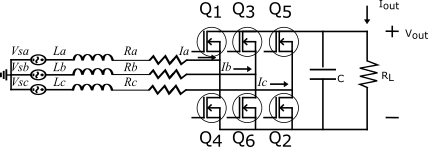
\includegraphics[width=\textwidth]{AFE_Final_Gates}
%	\caption{Active Front End Rectifier}
%	\label{fig:AFE_Modeling}
%\end{figure}
The grid voltage of each phase is described by a using KVL voltage equations that includes resistive drop of each boost inductor and the rate of change of flux linkage. This relationship is written in Equation~\eqref{eq:narr-abc-phase} for a generic phase and in Equation~\eqref{eq:narr-abc-vector} in vector form for all three phases. The resistive term represents the losses of the resistance of the boost inductor, while the derivative of flux linkage represents the boost inductor and its core losses.

\begin{table}[H]
\centering
\caption{Symbols used in the SPMSM model}
\label{tab:spmsm-notation-narrative}
\begin{tabular}{ll}
\hline
Symbol & Description \\
\hline
$R$ & Boost inductor resistance \\
$L$ &   Boost inductor inductance \\
$C$ &   DC Link Capacitor \\
$R_l$ & Load resistance \\
$v_a, v_b, v_c$ & Three phase grid voltages \\
$v_{conva}, v_{convb}, v_{convc}$ & Three phase converter voltages \\
$i_a, i_b, i_c$ & Three phase grid currents \\
$v_\alpha, v_\beta$ & Stationary-frame grid voltages \\
$v_{conv\alpha}, v_{conv\beta}$ & Stationary-frame converter voltages \\
$i_\alpha, i_\beta$ & Stationary-frame grid currents \\
$v_{sd}, v_{sq}$ & Synchronous dq frame grid voltages \\
$i_d, i_q$ & Synchronous dq frame currents \\
$v_{convd}, v_{convq}$ & Synchronous dq frame converter voltages \\
$v_{dc}$ & Output DC Link voltages \\
$s_d, s_q$ & Synchronous dq frame switching function \\
$\theta$ & Electrical angle \\
$\omega$ & Electrical frequency \\
$P$ & Three phase active power of the grid \\
$Q$ & Three phase reactive power of the grid \\

\hline
\end{tabular}
\end{table}

\begin{equation}
\label{eq:narr-abc-phase}
v_\ell - v_{conv\ell} = R\, i_\ell + L\frac{\mathrm di_\ell}{\mathrm d t} \,, \qquad \ell \in \{a,b,c\} .
\end{equation}

\begin{equation}
\label{eq:narr-abc-vector}
\begin{bmatrix} v_a \\ v_b \\ v_c \end{bmatrix} - 
\begin{bmatrix} v_{conva} \\ v_{convb} \\ v_{convc} \end{bmatrix}
= R \begin{bmatrix} i_a \\ i_b \\ i_c \end{bmatrix}
+ L\frac{\mathrm d}{\mathrm d t} \begin{bmatrix} i_a \\ i_b \\ i_c \end{bmatrix} .
\end{equation}

For active front end rectifier, the phase flux linkages consist of a  term proportional to phase current and an inductive term that depends on the inductance of the boost rectifier. Equations~\eqref{eq:narr-abc-phase}–\eqref{eq:narr-abc-vector} define the relationship between the three phase grid voltages and the three phase converter voltages by using KVL equations.

Applying the power‑invariant Clarke transform to Equations~\eqref{eq:narr-abc-phase}–\eqref{eq:narr-abc-vector} yields the stationary‑frame voltages in Equations~\eqref{eq:add-ab-volt-a} and \eqref{eq:add-ab-volt-b}. The resistive and inductive parts preserve their form under the linear transform. 

\begin{equation}
\label{eq:narr-clarke}
\begin{bmatrix} v_\alpha \\ v_\beta \end{bmatrix}
= \tfrac{2}{3}
\begin{bmatrix}
1 & -\tfrac{1}{2} & -\tfrac{1}{2} \\
0 & \tfrac{\sqrt 3}{2} & -\tfrac{\sqrt 3}{2}
\end{bmatrix}
\begin{bmatrix} v_a \\ v_b \\ v_c \end{bmatrix} .
\end{equation}

\begin{equation}
\label{eq:add-ab-volt-a}
 v_\alpha = R \, i_\alpha + L \, \frac{\mathrm d i_\alpha}{\mathrm d t} + v_{conv\alpha} .
\end{equation}
\begin{equation}
\label{eq:add-ab-volt-b}
 v_\beta = R \, i_\beta + L \, \frac{\mathrm d i_\beta}{\mathrm d t} + v_{conv\beta} .
\end{equation}

The Park transform rotates the stationary axes so that one axis is aligned with phase A. In this frame, steady operating points correspond to nearly constant quantities, which simplifies control and analysis. The mappings for current and voltage are given in Equations~\eqref{eq:narr-park-i} to \eqref{eq:narr-park-v}.

\begin{equation}
\label{eq:narr-park-i}
\begin{bmatrix} i_d \\ i_q \end{bmatrix}
= \begin{bmatrix} \cos \theta & \sin \theta \\ -\sin \theta & \cos \theta \end{bmatrix}
\begin{bmatrix} i_\alpha \\ i_\beta \end{bmatrix} .
\end{equation}

\begin{equation}
\label{eq:narr-park-v}
\begin{bmatrix} v_d \\ v_q \end{bmatrix}
= \begin{bmatrix} \cos \theta & \sin \theta \\ -\sin \theta & \cos \theta \end{bmatrix}
\begin{bmatrix} v_\alpha \\ v_\beta \end{bmatrix} .
\end{equation}

In the rotating frame, The direct- and quadrature-axis voltage balances are listed in Equations~\eqref{eq:narr-dq-vd} and \eqref{eq:narr-dq-vq}. The electrical angular frequency terms couple the axes and motivate decoupling in controllers.

\begin{equation}
\label{eq:narr-dq-vd}
v_{sd} = R\, i_d + \frac{\mathrm d i_d}{\mathrm d t} - \omega L i_q + v_{convd}.
\end{equation}

\begin{equation}
\label{eq:narr-dq-vq}
v_{sq} = R\, i_q + \frac{\mathrm d i_q}{\mathrm d t} + \omega L i_d + v_{convq}.
\end{equation}

Substituting the grid current derivative relations into the voltage balances leads to first-order dynamics for the axis currents. Equation~\eqref{eq:narr-dq-did} shows that the direct-axis current is driven by the direct-axis voltage, opposed by resistive drop, and coupled to the quadrature current through electrical frequency-dependent term. Equation~\eqref{eq:narr-dq-diq} shows that the quadrature-axis current is driven by the quadrature-axis voltage, opposed by resistive drop, and coupled to the quadrature current through electrical frequency-dependent term. These forms motivate feedforward decoupling in advanced controllers.

\begin{equation}
\label{eq:narr-dq-did}
\dot{i}_d = \frac{1}{L} \Big( v_{sd} - R i_d + \omega L i_q - v_{convd}\Big) .
\end{equation}

\begin{equation}
\label{eq:narr-dq-diq}
\dot{i}_q = \frac{1}{L} \Big( v_{sq} - R i_q - \omega L i_d - v_{convq}\Big) .
\end{equation}

The instantaneous three-phase electrical active power expressed in synchronous coordinates is a weighted inner product of voltage and current components, shown in Equation~\eqref{eq:narr-pe}. While The instantaneous three-phase electrical reactive power expressed in synchronous coordinates is a weighted inner product of voltage and current components, shown in Equation~\eqref{eq:narr-qe}.
\begin{equation}
\label{eq:narr-pe}
P = \tfrac{3}{2} \big( v_{sd} i_d + v_{sq} i_q \big) .
\end{equation}

\begin{equation}
\label{eq:narr-qe}
Q = \tfrac{3}{2} \big( v_{sq} i_d - v_{sd} i_q \big) .
\end{equation}


The above equations represent the instantaneous input active and reactive power supplied by the grid. Equation~\eqref{eq:narr-dclink} states the relation between the output DC link voltage and the output power drawn by the load. Those equations are necessary for the derivation of the transfer functions of the grid currents in the dq synchronous frame and the transfer function of the DC link voltage which are crucial for simulation and control design.

\begin{equation}
\label{eq:narr-dclink}
C\,\dot v_{dc} = \tfrac{3}{2} \big( S_d i_d + S_q i_q \big) - \frac{v_{dc}}{R_l} .
\end{equation}




% ==========================================================
% Subsection: Ideal Two-Level Inverter — Average (PWM) Model
% Requires: \usepackage{amsmath}
% ==========================================================

% ==========================================================
% Subsection: Ideal Two-Level Inverter — Average Model with SVM Duty Cycles
% Requires: \usepackage{amsmath}
% ==========================================================

% ==========================================================
% Subsection: Ideal Two-Level Inverter — Average Model Driven by SVM Duty Cycles
% Requires: \usepackage{amsmath}
% ==========================================================

\section{System Characterestics}
\label{subsec:motor-params-3col}

% In your preamble:
% \usepackage{booktabs}

% In your preamble:
% \usepackage{booktabs}

% Preamble: \usepackage{booktabs}
This subsection summarizes the parameters used throughout the modeling, control, and experiments as shown in  Table~\ref{tab:drive-motor-params};
\begin{table}[H]
	\centering
	\caption{Load and Active Front-End Rectifier parameters used in the experiments.}
	\label{tab:drive-motor-params}
	\begin{tabular}{l c r}
		\toprule
		\textbf{Parameter} & \textbf{Symbol} & \textbf{Value} \\
		\midrule
		DC Bus Voltage (V)                    & $V_{\mathrm{dc}}$    &600\\
		Switching Frequency (kHz)             & $f$                  &10  \\
		Dead Time ($\mu$s)                    & $T_{\mathrm{dead}}$  &2.5  \\
		Turn-on Time ($\mu$s)                 & $T_{\mathrm{ON}}$    &0.3  \\
		Turn-off Time ($\mu$s)                & $T_{\mathrm{OFF}}$   &0.3  \\
		Switch Threshold Voltage (V)          & $V_{\mathrm{ce0}}$   &0.4  \\
		Switch Turn-on Resistance ($\Omega$)  & $R_{\mathrm{ce}}$    &0.7  \\
		Diode Threshold Voltage (V)           & $V_{d0}$             &0.4  \\
		Diode Turn-on Resistance ($\Omega$)   & $R_d$                &0.7  \\
		\addlinespace[2pt]
		Inductor Resistance ($\Omega$)          & $R$                &0.55  \\
		Boost Inductor Inductance (H)               & $L$                &0.0185  \\
		Rated Supply Current per phase (A)                     & $I_{\mathrm{max}}$ &10 \\
		Rated Output Power (W)                   & $Pout_{\mathrm{rated}}$ &1200  \\
		Rated Load Current (A)                   & $I_{\mathrm{dcrated}}$ &2  \\
		\bottomrule
	\end{tabular}
\end{table}

\section{Vector Oriented Control (VOC)}
The foundation of the VOC strategy relies on the accurate synchronization with the AC grid, typically achieved through a Phase-Locked Loop (PLL). The PLL continuously extracts the grid voltage phase angle, establishing a reliable synchronization signal that allows the control system to align its rotating reference frame directly with the grid voltage vector. This precise alignment facilitates the core mechanism of VOC: the application of mathematical coordinate transformations to simplify time-varying, coupled three-phase signals. Specifically, the stationary three-phase grid variables—voltages and currents in the $abc$ frame—are first reduced to a two-phase orthogonal stationary frame (the $\alpha\beta$ frame) via the Clarke transformation. Subsequently, the Park transformation utilizes the PLL-derived phase angle to project these $\alpha\beta$ variables onto a synchronously rotating $dq$-axis reference frame.Within this synchronously rotating domain, the fundamental alternating grid variables appear as DC quantities in steady-state, which significantly simplifies the design and tuning of the linear controllers. Crucially, by aligning the $d$-axis perfectly with the grid voltage vector, the $q$-axis voltage component is inherently driven to zero. This mathematical alignment enables the complete decoupling of active and reactive power currents. Consequently, the $d$-axis current component ($i_d$) becomes directly proportional to the active power transferred, thereby dictating the DC-link voltage dynamics. Conversely, the $q$-axis current component ($i_q$) governs the reactive power exchange with the grid. By constraining the $q$-axis current reference to zero, the control system inherently achieves unity power factor operation.

Vector oriented control applies Clarke and Park transformations to convert the measured three-phase currents from the stationary \(abc\) frame into the synchronous \(dq\) frame for Grid Synchronisation. In that rotating frame, the grid currents appear as nearly dc quantities, which allows the grid current components in \(dq\) frame to be regulated independently using simple PI controllers. For the Active Front End Rectifier (AFE) considered here, the quadrature-axis current reference is typically set to \(i_q^{\ast}=0\) to eliminate the reactive power drawn from the grid, while the direct-axis current reference \(i_d^{\ast}\) is generated by the outer dc-link PI controller from the dc-link feedback measured. The inner \(d\)- and \(q\)-axis PI current controllers then generate the commanded voltages \(v_d^{\ast}\) and \(v_q^{\ast}\), which are transformed back to the stationary frame and synthesized by the rectifier using SVPWM. In VOC operation, the estimated electrical angle and electrical frequency supplied by the PLL are therefore essential because they define the transformation angle and preserve the decoupled current control structure. The system is shown in Figure \ref{fig:FocDiagram}.

\begin{figure}[h]
	\centering
	\resizebox{\textwidth}{!}{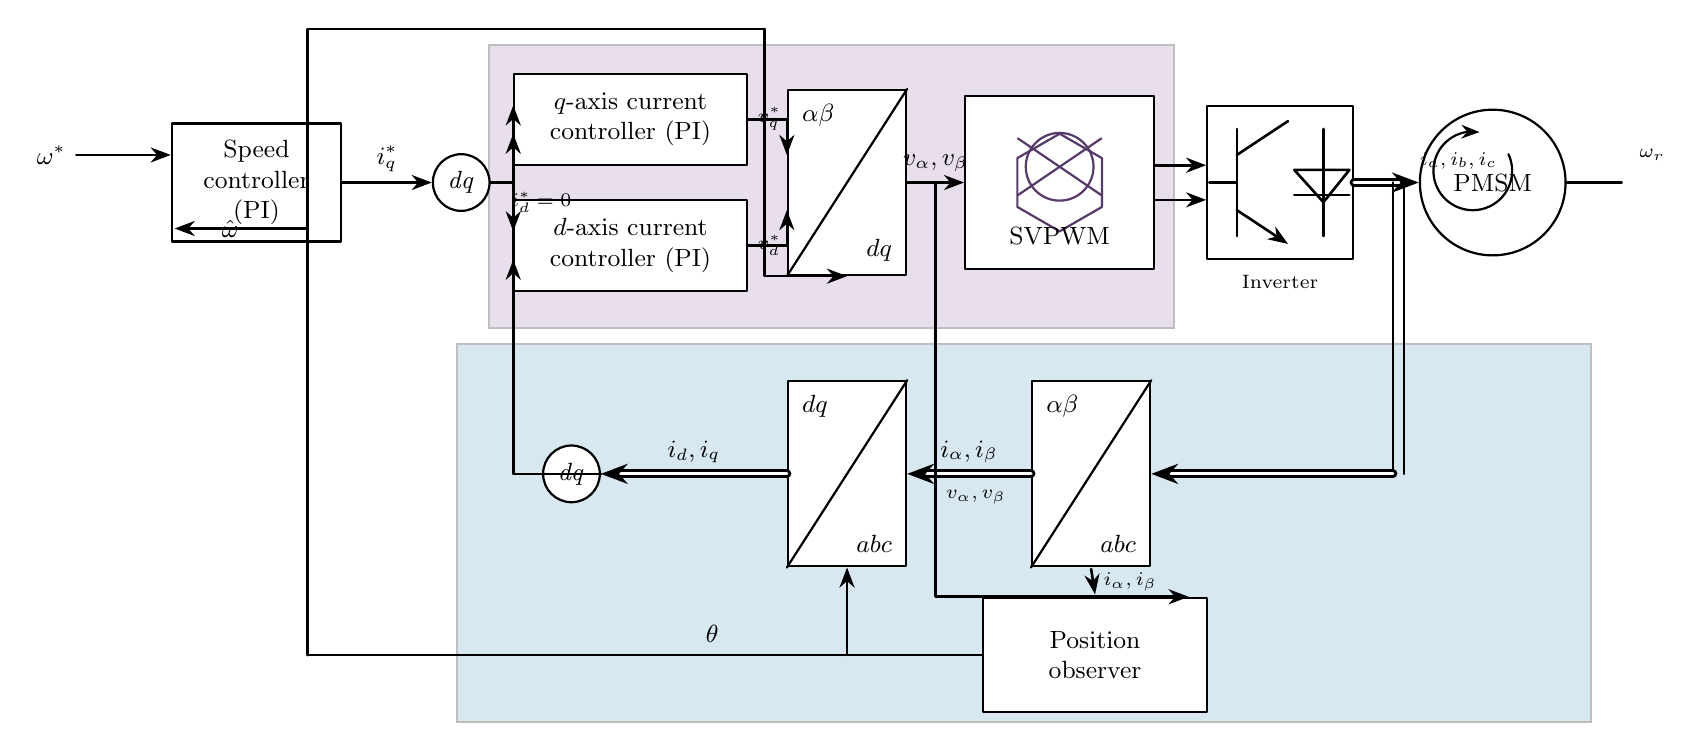
\begin{tikzpicture}[
    x=1cm,
    y=1cm,
    font=\small,
    >=Stealth,
    line cap=round,
    line join=round,
    signal/.style={->, line width=0.95pt},
    bus/.style={->, line width=1.05pt, double distance=1.15pt},
    plain/.style={line width=0.95pt},
    block/.style={draw, thick, fill=white, minimum width=2.45cm, minimum height=1.2cm, align=center},
    tallblock/.style={draw, thick, fill=white, minimum width=1.5cm, minimum height=2.35cm, inner sep=0pt},
    bubble/.style={circle, draw, thick, fill=white, minimum size=0.72cm, inner sep=0pt}
]

\definecolor{sensorpurple}{RGB}{233,222,236}
\definecolor{sensorblue}{RGB}{215,232,241}
\definecolor{svstroke}{RGB}{87,58,106}

\node[block, minimum width=2.15cm, minimum height=1.5cm] (speed) at (1.6,2.3) {Speed\\controller\\(PI)};

\node[bubble] (dqref) at (4.2,2.3) {$\mathit{dq}$};

\node[block, minimum width=2.95cm, minimum height=1.15cm] (qpi) at (6.35,3.1) {$q$-axis current\\controller (PI)};
\node[block, minimum width=2.95cm, minimum height=1.15cm] (dpi) at (6.35,1.5) {$d$-axis current\\controller (PI)};

\node[tallblock] (invpark) at (9.1,2.3) {};
\node[block, minimum width=2.4cm, minimum height=2.2cm] (svpwm) at (11.8,2.3) {};
\node[block, minimum width=1.85cm, minimum height=1.95cm] (inverter) at (14.6,2.3) {};

\node[circle, draw, thick, fill=white, minimum size=1.85cm, align=center] (pmsm) at (17.3,2.3) {PMSM};

\node[tallblock] (parkfb) at (9.1,-1.4) {};
\node[tallblock] (clarke) at (12.2,-1.4) {};
\node[bubble] (dqfb) at (5.6,-1.4) {$\mathit{dq}$};

\node[block, minimum width=2.85cm, minimum height=1.45cm] (observer) at (12.25,-3.7) {Position\\observer};

\begin{scope}[on background layer]
    \fill[sensorpurple] (4.55,4.05) rectangle (13.25,0.45);
    \fill[sensorblue] (4.15,0.25) rectangle (18.55,-4.55);
    \draw[black!25, thick] (4.55,4.05) rectangle (13.25,0.45);
    \draw[black!25, thick] (4.15,0.25) rectangle (18.55,-4.55);
\end{scope}

\draw[thick] (invpark.south west) -- (invpark.north east);
\node[anchor=north west] at ([xshift=2pt,yshift=-2pt]invpark.north west) {$\alpha\beta$};
\node[anchor=south east] at ([xshift=-2pt,yshift=2pt]invpark.south east) {$dq$};

\draw[thick] (parkfb.south west) -- (parkfb.north east);
\node[anchor=north west] at ([xshift=2pt,yshift=-2pt]parkfb.north west) {$dq$};
\node[anchor=south east] at ([xshift=-2pt,yshift=2pt]parkfb.south east) {$abc$};

\draw[thick] (clarke.south west) -- (clarke.north east);
\node[anchor=north west] at ([xshift=2pt,yshift=-2pt]clarke.north west) {$\alpha\beta$};
\node[anchor=south east] at ([xshift=-2pt,yshift=2pt]clarke.south east) {$abc$};

\begin{scope}[shift={(svpwm.center)}]
    \draw[thick, svstroke] (0,0.2) circle (0.43);
    \draw[thick, svstroke] (30:0.62)
        -- (90:0.62)
        -- (150:0.62)
        -- (210:0.62)
        -- (270:0.62)
        -- (330:0.62)
        -- cycle;
    \draw[thick, svstroke] (-0.53,-0.16) -- (0.53,0.56);
    \draw[thick, svstroke] (0.53,-0.16) -- (-0.53,0.56);
\end{scope}
\node[font=\small] at ($(svpwm.center)+(0,-0.68)$) {SVPWM};

\begin{scope}[shift={(inverter.center)}, line width=0.95pt]
    \draw (-0.55,0.68) -- (-0.55,-0.68);
    \draw (-0.90,0.00) -- (-0.55,0.00);
    \draw (-0.55,0.35) -- (0.10,0.78);
    \draw[-Stealth] (-0.55,-0.35) -- (0.10,-0.78);
    \draw (0.55,0.68) -- (0.55,-0.68);
    \draw (0.18,0.16) -- (0.88,0.16) -- (0.55,-0.25) -- cycle;
    \draw (0.18,-0.16) -- (0.88,-0.16);
\end{scope}
\node[font=\scriptsize, below=2pt of inverter] {Inverter};

\draw[thick] (pmsm.east) -- ++(0.7,0);
\draw[thick, ->] ($(pmsm.center)+(0.20,0.36)$) arc[start angle=25,end angle=-280,radius=0.50];
\node[font=\scriptsize, right] at ($(pmsm.east)+(0.8,0.35)$) {$\omega_r$};

\draw[signal] ($(speed.west)+(-1.2,0.35)$) node[left] {$\omega^{\ast}$} -- ($(speed.west)+(0,0.35)$);
\draw[signal] (speed.east) -- node[above] {$i_q^{\ast}$} (dqref.west);

\draw[signal] (dqref.east) -| ($(qpi.west)+(0,0.18)$);
\draw[signal] (dqref.east) -| ($(dpi.west)+(0,0.18)$);
\node[font=\scriptsize, anchor=west] at ($(dpi.west)+(-0.15,0.55)$) {$i_d^{\ast}=0$};

\draw[signal] (qpi.east) -| ($(invpark.west)+(0,0.35)$);
\draw[signal] (dpi.east) -| ($(invpark.west)+(0,-0.35)$);
\node[font=\scriptsize, anchor=south] at ($(qpi.east)!0.55!(invpark.west)+(0,0.18)$) {$v_q^{\ast}$};
\node[font=\scriptsize, anchor=north] at ($(dpi.east)!0.55!(invpark.west)+(0,-0.18)$) {$v_d^{\ast}$};

\coordinate (vabmid) at ($(invpark.east)!0.5!(svpwm.west)$);
\draw[signal] (invpark.east) -- node[above] {$v_{\alpha},v_{\beta}$} (svpwm.west);

\draw[signal] ($(svpwm.east)+(0,0.22)$) -- ($(inverter.west)+(0,0.22)$);
\draw[signal] ($(svpwm.east)+(0,-0.22)$) -- ($(inverter.west)+(0,-0.22)$);

\draw[bus] (inverter.east) -- (pmsm.west);

\coordinate (meastop) at ($(inverter.east)!0.60!(pmsm.west)$);
\coordinate (measbot) at ($(meastop |- clarke.east)$);

\draw[line width=1.0pt] (meastop) -- (measbot);
\draw[line width=1.0pt] ($(meastop)+(0.14,0)$) -- ($(measbot)+(0.14,0)$);
\node[font=\scriptsize, anchor=west] at ($(meastop)+(0.22,0.28)$) {$i_a,i_b,i_c$};

\draw[bus] (measbot) -- (clarke.east);
\draw[bus] (clarke.west) -- node[above] {$i_{\alpha},i_{\beta}$} (parkfb.east);
\draw[bus] (parkfb.west) -- node[above] {$i_d,i_q$} (dqfb.east);

\draw[signal] (dqfb.east) -| ($(qpi.west)+(0,-0.18)$);
\draw[signal] (dqfb.east) -| ($(dpi.west)+(0,-0.18)$);

\draw[signal] ($(clarke.south)+(0,-0.02)$) -- node[right, font=\scriptsize] {$i_{\alpha},i_{\beta}$} ($(observer.north)+(0,0.03)$);
\draw[signal] (vabmid) |- node[pos=0.38, right, font=\scriptsize] {$v_{\alpha},v_{\beta}$} ($(observer.north east)+(-0.25,0)$);

\coordinate (thetal) at (2.25,-3.7);
\coordinate (thetahub) at (9.1,-3.7);
\coordinate (thetaup) at (2.25,4.25);
\coordinate (thetatop) at (8.05,4.25);

\draw[plain] (observer.west) -- (thetal);
\node[font=\small] at ($(observer.west)!0.40!(thetal)+(0,0.27)$) {$\theta$};

\draw[signal] (thetahub) -- (parkfb.south);
\draw[plain] (thetal) -- (thetaup) -- (thetatop);
\draw[signal] (thetatop) |- (invpark.south);
\draw[signal] (thetal) |- node[pos=0.72, left] {$\hat{\omega}$} ($(speed.south west)+(0.05,0.18)$);

\end{tikzpicture}}
	\caption{Sensorless Drive System}
	\label{fig:FocDiagram}
\end{figure}

% =====================================================================
% Subsection: Sliding-Mode Observer (SMO) for SPMSM — αβ-frame derivation
% Drop into your Sensorless chapter/section. No web refs; cite your own [Krause, Vas]
% Requires: \usepackage{amsmath,amssymb,bm}
% Optional: \numberwithin{equation}{chapter}
% Policy: minimal inline math; all key formulas displayed and labeled.
% =====================================================================

\subsection{Sliding-Mode Observer (SMO) in the \texorpdfstring{$\alpha\beta$}{alpha--beta} Frame}
\label{subsec:smo-ab}

The SMO estimates rotor electrical angle and speed without mechanical sensors by reconstructing the back-electromotive-force (back-EMF) vector from measured stator currents and applied voltages. The observer is formulated in the stationary \(\alpha\beta\) frame for a surface-mounted PMSM (isotropic inductance). In all derivations below, the voltages fed to the observer are the inverter-compensated \(\alpha\beta\) voltages produced by the non-linearity map, which reduces bias at low speed.

The electrical dynamics in the stationary frame are
\begin{equation}
	\label{eq:smo-plant-alphabeta}
	\begin{bmatrix} v_\alpha \\ v_\beta \end{bmatrix}
	= R_s \begin{bmatrix} i_\alpha \\ i_\beta \end{bmatrix}
	+ L_s \frac{\mathrm d}{\mathrm d t} \begin{bmatrix} i_\alpha \\ i_\beta \end{bmatrix}
	+ \begin{bmatrix} e_\alpha \\ e_\beta \end{bmatrix} .
\end{equation}
The back-EMF components due to the permanent magnet are
\begin{equation}
	\label{eq:smo-emf-ab}
	e_\alpha = -\lambda_f\,\omega_e\,\sin\theta_e\,,\qquad e_\beta = \lambda_f\,\omega_e\,\cos\theta_e\,.
\end{equation}
Dividing the two components and using the inverse tangent yields the electrical angle
\begin{equation}
	\label{eq:smo-angle-from-emf}
	\theta_e = \operatorname{atan2}\big(-e_\alpha,\,e_\beta\big).
\end{equation}
Solving \eqref{eq:smo-plant-alphabeta} for the current derivatives gives
\begin{equation}
	\label{eq:smo-plant-dynamics}
	\frac{\mathrm d}{\mathrm d t} \begin{bmatrix} i_\alpha \\ i_\beta \end{bmatrix}
	= -\frac{R_s}{L_s} \begin{bmatrix} i_\alpha \\ i_\beta \end{bmatrix}
	+ \frac{1}{L_s} \begin{bmatrix} v_\alpha \\ v_\beta \end{bmatrix}
	- \frac{1}{L_s} \begin{bmatrix} e_\alpha \\ e_\beta \end{bmatrix} .
\end{equation}

Define the current-estimation errors and sliding surfaces as
\begin{equation}
	\label{eq:smo-sliding-surfaces}
	\tilde i_\alpha = i_\alpha - \hat i_\alpha\,,\qquad \tilde i_\beta = i_\beta - \hat i_\beta\,,\qquad S_\alpha=\tilde i_\alpha\,,\; S_\beta=\tilde i_\beta\,.
\end{equation}
The SMO injects a discontinuous term to drive \(S\to 0\). A practical implementation uses a boundary layer via \(\operatorname{sat}(\cdot)\) in place of \(\operatorname{sgn}(\cdot)\). The observer dynamics are
\begin{equation}
	\label{eq:smo-observer-dynamics}
	\frac{\mathrm d}{\mathrm d t} \begin{bmatrix} \hat i_\alpha \\ \hat i_\beta \end{bmatrix}
	= -\frac{R_s}{L_s} \begin{bmatrix} \hat i_\alpha \\ \hat i_\beta \end{bmatrix}
	+ \frac{1}{L_s} \begin{bmatrix} v_\alpha \\ v_\beta \end{bmatrix}
	+ \frac{\eta_0}{L_s}
	\begin{bmatrix}
		\operatorname{sgn}\!\left(\tfrac{\tilde i_\beta}{\varphi}\right) \\ 
		\operatorname{sgn}\!\left(\tfrac{\tilde i_\beta}{\varphi}\right)
	\end{bmatrix} ,
\end{equation}
where \(\eta_0>0\) is the switching gain.

Subtracting \eqref{eq:smo-observer-dynamics} from \eqref{eq:smo-plant-dynamics} yields
\begin{equation}
	\label{eq:smo-error-dynamics}
	\frac{\mathrm d}{\mathrm d t} \begin{bmatrix} \tilde i_\alpha \\ \tilde i_\beta \end{bmatrix}
	= -\frac{R_s}{L_s} \begin{bmatrix} \tilde i_\alpha \\ \tilde i_\beta \end{bmatrix}
	+ \frac{1}{L_s} \begin{bmatrix} e_\alpha \\ e_\beta \end{bmatrix}
	- \frac{\eta_0}{L_s}
	\begin{bmatrix}
		\operatorname{sgn}(\tilde i_\alpha) \\ 
		\operatorname{sgn}(\tilde i_\beta)
	\end{bmatrix} .
\end{equation}
Using the Lyapunov candidate \(V = \tfrac{1}{2}(S_\alpha^2+S_\beta^2)\), the condition
\begin{equation}
	\label{eq:smo-sliding-condition}
	S_\alpha\,\dot S_\alpha + S_\beta\,\dot S_\beta \le 0
\end{equation}
holds whenever the switching gain exceeds the worst-case mismatch in back-EMF estimation, i.e., when
\begin{equation}
	\label{eq:smo-eta-condition}
	\eta_0 > \max\big\{\,|e_\alpha|,\; |e_\beta|\,\big\}\,.
\end{equation}
Under \eqref{eq:smo-eta-condition} and bounded inputs, the surfaces are reached in finite time.

The discontinuous term approximates the unknown disturbance vector \(\mathbf{e}\). Its components are
\begin{equation}
	\label{eq:smo-e-vector}
	\mathbf{e} = \begin{bmatrix} e_\alpha \\ e_\beta \end{bmatrix} .
\end{equation}
A smooth estimate is obtained by low-pass filtering the switching action:
\begin{equation}
	\label{eq:smo-emf-estimate}
	\begin{bmatrix} \hat e_\alpha \\ \hat e_\beta \end{bmatrix}
	= \operatorname{LPF}\left\{\, \eta_0
	\begin{bmatrix}
		\operatorname{sgn}(\tilde i_\alpha) \\ 
		\operatorname{sgn}(\tilde i_\beta)
	\end{bmatrix}\,\right\} .
\end{equation}
A second-order low-pass filter is preferred to reduce ripple and phase lag at the switching frequency; a cutoff one decade below the PWM carrier and above the fundamental improves noise immunity while preserving dynamics.

The electrical angle is computed from the estimated back-EMF components as
\begin{equation}
	\label{eq:smo-angle-est}
	\hat \theta_e = \operatorname{atan2}\big(-\hat e_\alpha,\,\hat e_\beta\big) .
\end{equation}
Speed may be obtained by differentiating \(\hat \theta_e\) or, more robustly, by a synchronous-frame PLL driven by the quadrature back-EMF component; both methods are compatible with the observer.

The LPF cutoff should be chosen high enough to capture back-EMF dynamics during transients yet low enough to reject the switching ripple introduced by \(\operatorname{sgn}(\cdot)\).

The SMO proceeds as follows: integrate \eqref{eq:smo-observer-dynamics} each sampling period using the compensated \(\alpha\beta\) voltages; reconstruct back-EMF via \eqref{eq:smo-emf-estimate}; compute angle via \eqref{eq:smo-angle-est}; and update speed using a PLL or filtered differentiation. Feeding compensated voltages minimizes bias from inverter non-idealities and stator-resistance drift, which is critical at low speed.

To guarantee a constant phase relationship between the estimated back-EMF and the fundamental, two adaptive first-order low-pass filters are cascaded with identical cutoff frequencies scheduled from the instantaneous electrical speed. The phase of a first-order LPF at angular frequency is
\begin{equation}
	\label{eq:smo-lpf-phase}
	\phi(\omega) = -\arctan\!\left(\frac{\omega}{\omega_c}\right).
\end{equation}
Choosing the cutoff equal to the electrical speed enforces a fixed per-stage phase at the fundamental:
\begin{equation}
	\label{eq:smo-lpf-choice}
	\omega_c = |\omega_e|.
\end{equation}
Evaluating \eqref{eq:smo-lpf-phase} at the electrical frequency gives
\begin{equation}
	\label{eq:smo-lpf-45}
	\phi(\omega_e) = -\arctan(1) = -45^{\circ}.
\end{equation}
Therefore, the cascade produces approximately a $-90^{\circ}$ total phase shift at the fundamental as shown Figure \ref{fig:FilterResponse} in while continuing to attenuate switching ripple.

\begin{figure}[h]
	\centering
	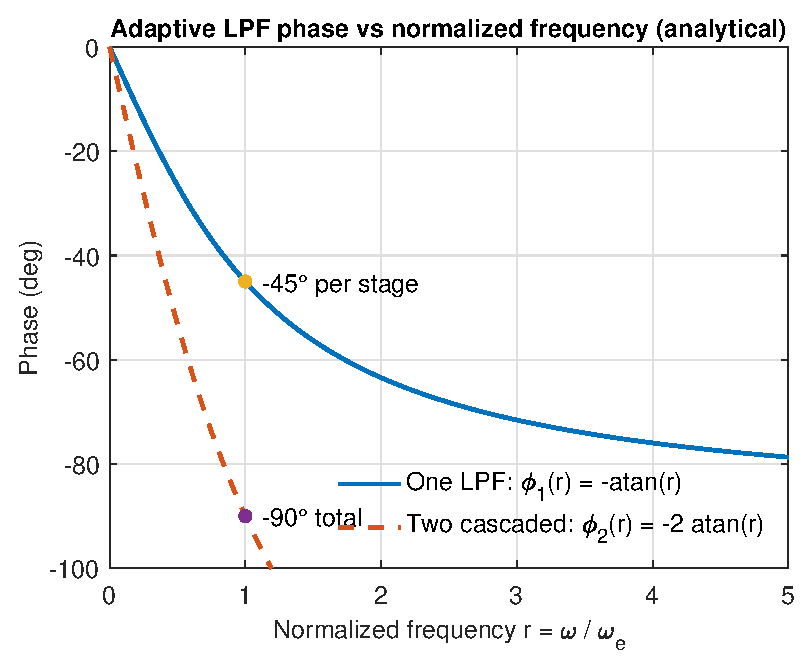
\includegraphics[width=\textwidth]{./Filter}
	\caption{Cascaded First Order Filter Response}
	\label{fig:FilterResponse}
\end{figure}

Let the switching action be
\[
\mathbf s = \eta_0\,
\begin{bmatrix}
	\operatorname{sgn}(\tilde i_\alpha) \\ 
	\operatorname{sgn}(\tilde i_\beta)
\end{bmatrix}.
\]

The cascaded filters are
\begin{equation}
	\label{eq:smo-lpf1}
	\dot{\mathbf z}_1 = -2\pi\, f_c(\omega_e)\, \mathbf z_1 + 2\pi\, f_c(\omega_e)\, \mathbf s ,
\end{equation}
\begin{equation}
	\label{eq:smo-lpf2}
	\dot{\mathbf z}_2 = -2\pi\, f_c(\omega_e)\, \mathbf z_2 + 2\pi\, f_c(\omega_e)\, \mathbf z_1 ,
\end{equation}
\begin{equation}
	\label{eq:smo-ehat-cascade}
	\begin{bmatrix} \hat e_\alpha \\ \hat e_\beta \end{bmatrix} = \mathbf z_2 .
\end{equation}
The speed-scheduled cutoff is
\begin{equation}
	\label{eq:smo-fc-omega}
	f_c(\omega_e) = \operatorname{clip}\!\Big( \tfrac{|\omega_e|}{2\pi} ,\; f_{\min} ,\; \min\{ f_{\max} ,\, f_{\mathrm{PWM}}/10 \} \Big) .
\end{equation}


% =====================================================================
% Subsection: Speed Estimation from Estimated Electrical Angle
% Context: angle \hat\theta_e is available from atan2 on the back-EMF vector
% Policy: minimal inline math; key formulas displayed and labeled
% Requires: \usepackage{amsmath,amssymb}
% =====================================================================

% =====================================================================
% Subsection: Speed Estimation from Estimated Electrical Angle — Simple 1st-Order LPF
% Replaces the previous smoothing (Tustin) with a single-coefficient recursion
% Requires: \usepackage{amsmath,amssymb}
% =====================================================================

\subsection{Speed Estimation from the Estimated Electrical Angle}
\label{subsec:speed-from-angle-simple}


This subsection computes electrical and mechanical speed from the estimated electrical angle obtained via the arctangent of the back-EMF vector. A plain differentiator is used, followed by a simple first-order low-pass filter applied only to the speed.


The estimator assumes a uniformly sampled angle sequence with sampling period shown in \eqref{eq:spdS-Ts}.
\begin{equation}
	\label{eq:spdS-Ts}
	T_s > 0 .
\end{equation}
The wrapped electrical angles are denoted in \eqref{eq:spdS-theta}.
\begin{equation}
	\label{eq:spdS-theta}
	\hat\theta_e[k] \in (-\pi,\,\pi] ,\qquad k=0,1,2,\dots
\end{equation}


Let the raw sample–to–sample angle difference be
\begin{equation}
	\label{eq:spd-dtheta-raw}
	\Delta\theta_{\mathrm{raw}}[k] = \hat\theta_e[k] - \hat\theta_e[k-1] .
\end{equation}
To suppress the $\pm 2\pi$ wrap, compare $\Delta\theta_{\mathrm{raw}}[k]$ with a limit
$\Delta\theta_{\lim}\in(\tfrac{\pi}{2},\,\pi]$ and correct as
\begin{equation}
	\label{eq:spd-dtheta-limited}
	\Delta\theta_e[k] =
	\begin{cases}
		\Delta\theta_{\mathrm{raw}}[k] - 2\pi, & \Delta\theta_{\mathrm{raw}}[k] > \Delta\theta_{\lim},\\[4pt]
		\Delta\theta_{\mathrm{raw}}[k] + 2\pi, & \Delta\theta_{\mathrm{raw}}[k] < -\,\Delta\theta_{\lim},\\[4pt]
		\Delta\theta_{\mathrm{raw}}[k], & \text{otherwise.}
	\end{cases}
\end{equation}
The electrical speed estimate then is
\begin{equation}
	\label{eq:spd-omega-from-dtheta}
	\hat\omega_e[k] = \frac{\Delta\theta_e[k]}{T_s}.
\end{equation}
the sampling period satisfies
\begin{equation}
	\label{eq:spd-sampling-bound}
	T_s < \frac{\Delta\theta_{\lim}}{\omega_{e,\max}}
	\quad\Big(\text{equivalently } f_s > \omega_{e,\max}/\Delta\theta_{\lim}\Big),
\end{equation}
so that genuine inter-sample motion never exceeds the limit and only wrap events are corrected.



The raw electrical speed estimate is then
\begin{equation}
	\label{eq:spdS-omega-raw}
	\hat\omega_e[k] = \frac{\Delta\theta_e[k]}{T_s} .
\end{equation}


The raw speed \(\hat\omega_e[k]\) is smoothed by a single-coefficient recursion as in \eqref{eq:spdS-simple-lpf}. This is the discrete first-order low-pass filter you requested ("\(Y[k]=G\,Y[k-1]+(1-G)U[k]\)") with input \(U[k]=\hat\omega_e[k]\) and output \(Y[k]=\omega_{e,f}[k]\).
\begin{equation}
	\label{eq:spdS-simple-lpf}
	\omega_{e,f}[k] = G\; \omega_{e,f}[k-1] + (1-G)\; \hat\omega_e[k] .
\end{equation}
Two equivalent expressions for the filter coefficient are commonly used:
\begin{equation}
	\label{eq:spdS-G-exact}
	G = e^{-\omega_c T_s} ,
\end{equation}
\begin{equation}
	\label{eq:spdS-G-approx}
	G \approx \frac{1}{1 + \omega_c T_s} \quad \text{for small } \omega_c T_s .
\end{equation}
Equation \eqref{eq:spdS-G-exact} is the exact zero-order-hold discretization of a first-order lag with cutoff \(\omega_c\); Equation \eqref{eq:spdS-G-approx} is a convenient algebraic approximation giving nearly identical factors when \(\omega_c T_s\ll 1\).

Mechanical speed and revolutions per minute follow from \eqref{eq:spdS-omegam} and \eqref{eq:spdS-rpm} using the number of pole pairs \(p\).
\begin{equation}
	\label{eq:spdS-omegam}
	\hat\omega_m[k] = \frac{\omega_{e,f}[k]}{p} .
\end{equation}
\begin{equation}
	\label{eq:spdS-rpm}
	\hat n[k] = \frac{60}{2\pi} \, \hat\omega_m[k] .
\end{equation}


% =====================================================================
% Subsection: PI Field-Oriented Speed Controller — Pole-Placement Design
% Context: SPMSM, i_d ≈ 0, fast inner current loops (i_q tracking ≈ ideal)
% Requires: \usepackage{amsmath,amssymb}
% Policy: keep equations displayed and labeled; prose explains each step
% =====================================================================

% =====================================================================
% Subsection: FOC Speed PI via Pole Placement (Series topology C(s)=k_p(1+k_i/s))
% Requires: \usepackage{amsmath,amssymb}
% =====================================================================

% =====================================================================
% Subsection: PI Speed Controller by Pole Cancellation (Series topology)
% Requires: \usepackage{amsmath,amssymb}
% =====================================================================

% =====================================================================
% Subsection: Series PI Speed Controller by Pole Cancellation (Design Story)
% Requires: \usepackage{amsmath,amssymb}
% =====================================================================

\section{Transfer functions and System Parameters}
\label{subsec:Transfer-Functions}
\subsection{Series PI Current Controller by Pole Cancellation}
\label{subsec:pi-current-series-pc}


For control design and analysis, the inverter is represented by an average model over each PWM period. After using decoupling due to presence of $\omega$L terms, equations \eqref{eq:narr-dq-vd} and \eqref{eq:narr-dq-vq} can be decoupled as follows:

\begin{equation}
	\label{eq:idcurr-dq}
	L\frac{\mathrm d i_d}{\mathrm d t} = (R\, + Rce) i_d + v^{*}_{d}.
\end{equation}

\begin{equation}
	\label{eq:iqcurr-dq}
	L\frac{\mathrm d i_q}{\mathrm d t} = (R\, + Rce) i_q + v^{*}_{q}.
\end{equation}

Where $v^{*}_{d}$ and $v^{*}_{q}$ can be described as the voltage references which represent the PI control actions in the synchronous dq reference frame from which the grid currents $id$ and $iq$ can be controlled.

From equations \eqref{eq:narr-dq-vd} and \eqref{eq:narr-dq-vq}, the transfer function of the inner current loops for the grid currents can be expressed in Laplace Domain in the synchronous dq frame as follows:

\begin{equation}
	\label{eq:cur-Gp}
	G_i(s) \;=\; \frac{I(s)}{U(s)} \;=\; \frac{1}{L\, s + (R\, + Rce)} .
\end{equation}

Use the series PI topology on both axes:
\begin{equation}
	\label{eq:cur-C}
	C(s) \;=\; k_p \left( 1 + \frac{k_i}{s} \right) \;=\; k_p\,\frac{s + k_i}{s} .
\end{equation}
Place the controller zero on the plant pole:
\begin{equation}
	\label{eq:curr-cancell}
	k_i \;=\; \frac{R}{L} .
\end{equation}
With \eqref{eq:curr-cancell}, the loop reduces to a pure integrator gain:
\begin{equation}
	\label{eq:cur-loop}
	L(s) \;=\; C(s)\,G_i(s) \;=\; \frac{k_p}{L}\,\frac{1}{s} .
\end{equation}

Select the desired closed-loop bandwidth (per axis):
\begin{equation}
	\label{eq:cur-wc}
	\omega_{ci} \;>\; 0 , \qquad \tau_i \;=\; \frac{1}{\omega_{ci}} .
\end{equation}
The proportional gain that realizes \eqref{eq:cur-wc} is
\begin{equation}
	\label{eq:cur-kp}
	k_p \;=\; L\, \omega_{ci} \;=\; \frac{L}{\tau_i} .
\end{equation}
Equations \eqref{eq:curr-cancell}–\eqref{eq:cur-kp} produce a first-order, monotonic current response with zero steady-state error to step references (neglecting saturation).


For each axis, define the error, the integrator state, and the auxiliary control:
\begin{equation}
	\label{eq:cur-realize}
	e_d = i_d^{\ast} - i_d , \qquad \dot{x}_{I,d} = k_i\, e_d , \qquad u_d = k_p\,(e_d + x_{I,d}) ,
\end{equation}
\begin{equation}
	\label{eq:cur-realize-q}
	e_q = i_q^{\ast} - i_q , \qquad \dot{x}_{I,q} = k_i\, e_q , \qquad u_q = k_p\,(e_q + x_{I,q}) .
\end{equation}
Recover the commanded dq voltages for the PWM modulator:
\begin{equation}
	\label{eq:cur-vdcmd}
	v_d^{\ast} \;=\; u_d \;-\; \omega_e\, L_s\, i_q ,
\end{equation}
\begin{equation}
	\label{eq:cur-vqcmd}
	v_q^{\ast} \;=\; u_q \;+\; \omega_e\, L_s\, i_d .
\end{equation}


Limit the voltage vector to the available DC bus (space-vector circle limitation):
\begin{equation}
	\label{eq:cur-sat}
	\begin{bmatrix} v_d^{\ast\,\mathrm{sat}} \\[2pt] v_q^{\ast\,\mathrm{sat}} \end{bmatrix}
	= \operatorname{sat}_{V_{\max}}\!\left( \begin{bmatrix} v_d^{\ast} \\ v_q^{\ast} \end{bmatrix} \right) ,
	\qquad V_{\max} \approx \frac{V_{\mathrm{dc}}}{\sqrt{3}} .
\end{equation}
Apply back-calculation anti-windup on each axis using the voltage deficit:
\begin{equation}
	\label{eq:cur-aw-d}
	\dot{x}_{I,d} \;=\; k_i\, e_d \;+\; \frac{K_{aw}}{k_p}\,\big( v_d^{\ast\,\mathrm{sat}} - v_d^{\ast} \big) ,
\end{equation}
\begin{equation}
	\label{eq:cur-aw-q}
	\dot{x}_{I,q} \;=\; k_i\, e_q \;+\; \frac{K_{aw}}{k_p}\,\big( v_q^{\ast\,\mathrm{sat}} - v_q^{\ast} \big) .
\end{equation}


The $d$- and $q$-axis series PI controllers are tuned by pole cancellation, placing the controller zero at the plant pole and using the proportional gain to set a first-order closed-loop pole. With $L=0.018585~\mathrm{H}$ and $R = 0.55~\Omega$, and choosing a closed-loop bandwidth of $f_{ci}=100~\mathrm{Hz}$ as shown in \ref{fig:CurrentControllerBodePlot},
\begin{equation}
	\label{eq:cur-wci-num}
	\omega_{ci} = 2\pi\cdot 100 = 628.31853~\text{rad/s}, \qquad \tau_i=\frac{1}{\omega_{ci}}=1.5915\times 10^{-3}~\text{s},
\end{equation}
\begin{equation}
	\label{eq:cur-ki-num}
	k_{i,d}=k_{i,q}=\frac{R_s}{L}=\frac{0.55}{0.018585}=29.594~\text{rad/s},
\end{equation}
\begin{equation}
	\label{eq:cur-kp-num}
	k_{p,d}=k_{p,q}=L\,\omega_{ci}=0.018585\times 628.31853=11.677~.
\end{equation}
This yields identical first-order closed-loop dynamics on both axes with time constant $\tau_i\approx1.5915$\,ms and zero steady-state error to step current commands. (If a different $f_{ci}$ is adopted, recompute only $k_{p,\{\!d,q\!\}}=L\,\omega_{ci}$ while keeping $k_{i,\{\!d,q\!\}}=R/L$.)

\begin{figure}[H]
	\centering
	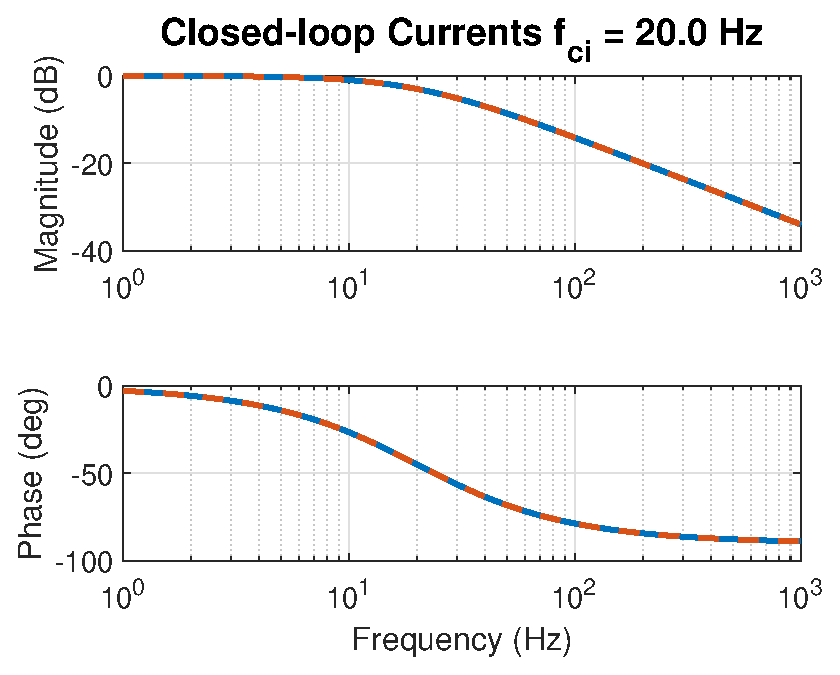
\includegraphics[width=\textwidth]{./CurrentControllerBodePlot}
	\caption{DQ-Axes Controller Design Bode Plot}
	\label{fig:CurrentControllerBodePlot}
\end{figure}

\subsection{Series PI DC-Link Voltage Controller by Pole Cancellation}
\label{subsec:pi-vdc-series-pc}


The outer DC-Link Voltage loop commands the direct–current reference so that the DC-Link Voltage requested by the load tracks its reference. The inner current loops are assumed fast, therefore the direct current tracks its command with negligible dynamics. A series PI is adopted and tuned to have narrower bandwidth (or slower time constant) than the current loop.

By using the balance for the active power given in \eqref{eq:narr-pe}: 
\begin{equation}
	\label{eq:pc-dc}
	\hat{P} = V_{sd}\hat{I_{d}} + V_{sq}\hat{I_{q}} +\tfrac{L}{2}\,\tfrac{d(\hat{I_{d}^2}+\hat{I_{q}^2})}{dt}\ = \tfrac{C}{2}\,\tfrac{d(\hat{V_{dc}^2})}{dt}\ + \hat{V_{dc}}I_{dc} 
\end{equation}

The transfer function between the DC-Link voltage and the grid current in D-axis can be derived from \eqref{eq:pc-dc} as follows:
\begin{equation}
	\label{eq:pc-Gvdc}
	G_{d}(s) = \tfrac{\hat{Vdc}}{\hat{Id}} = \tfrac{-sLId+V_{sd}}{sCV_{dc}+I_{dc}}.
\end{equation}

The series PI is written as
\begin{equation}
	\label{eq:pc-controller}
	C(s) = k_p\!\left(1 + \frac{k_i}{s}\right) = k_p\,\frac{s + k_i}{s} .
\end{equation}
%The controller zero is placed to cancel the plant pole by setting
%\begin{equation}
%	\label{eq:pc-cancel}
%	k_i = \frac{B}{J} .
%\end{equation}
With \eqref{eq:pc-Gvdc}, the loop gain with voltage transfer function has 2 poles and a RHP zero. 

The closed loop from DC-Link Voltage reference reduces to first order by the assumption of fast inner current loop.

The speed loop bandwidth and time constant are chosen explicitly as
\begin{equation}
	\label{eq:pc-wc}
	\omega_c > 0 , \qquad \tau = \frac{1}{\omega_c} .
\end{equation}

Define the speed error and the PI internal state and torque command as
\begin{equation}
	\label{eq:pc-realize}
	e_{V_{dc}} = V_{dcref}^{*} - V_{dc}.
\end{equation}
The direct–current command follows from the control action of the outer DC-Link Voltage. The commanded current is limited to the available range:

\begin{equation}
	\label{eq:pc-sat}
	i_d^{\ast\,\mathrm{sat}} = \operatorname{sat}\!\big(i_d^{\ast};\, -i_{d,\max},\, i_{d,\max}\big).
\end{equation}

In this work, the series PI speed controller is tuned for a closed-loop bandwidth of 10\,Hz as shown in Figure\ref{fig:SpeedControllerBodePlot}, ensuring clear separation from the inner current loops while preserving ripple free DC-Link Voltage. Using the pole-cancellation design, the controller zero is placed at the mechanical pole and the proportional gain sets the first-order closed-loop pole. The design values are:
\begin{equation}
	\label{eq:speed-wc-num}
	\omega_c = 2\pi\cdot 10 = 62.832~\text{rad/s}, \qquad \tau=\frac{1}{\omega_c}=0.01592~\text{s},
\end{equation}
%\begin{equation}
%	\label{eq:kt-num}
%	K_t = \tfrac{3}{2}\,p\,\lambda_f = \tfrac{3}{2}\cdot 4 \cdot 0.1227 = 0.7362~\text{N\,m/A},
%\end{equation}
\begin{equation}
	\label{eq:ki-num}
	k_i = 1.5~\text{rad/s},
\end{equation}
\begin{equation}
	\label{eq:kp-num}
	k_p = 0.25.
\end{equation}
With \(k_i\) and \(k_p\) as above, the closed-loop speed response is first-order with time constant \(\tau\approx 0.0159\) s and zero steady-state error to step commands with proper dynamics with a suitable bandwidth from the bandwidth of the current controllers.

\begin{figure}[h]
	\centering
	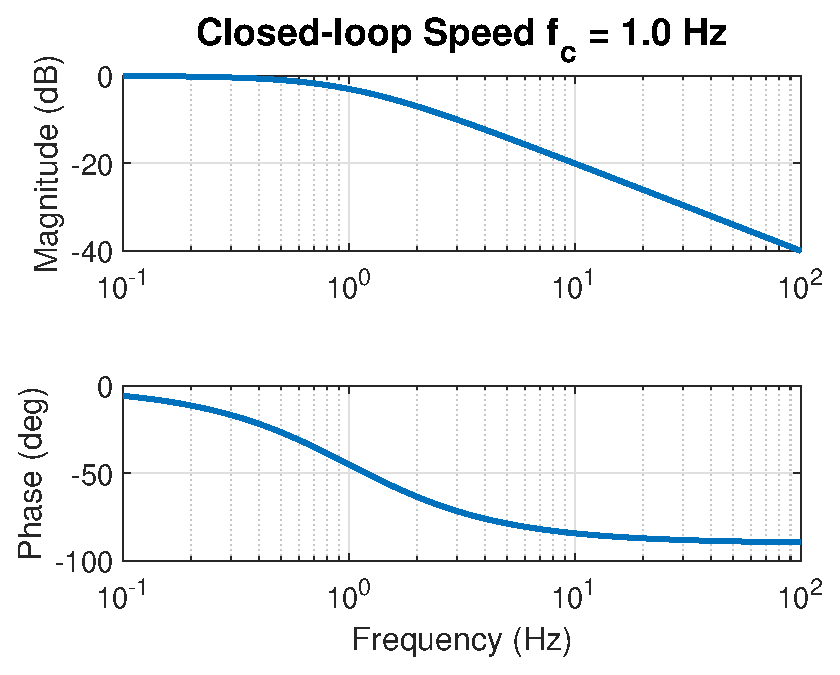
\includegraphics[width=\textwidth]{./SpeedControllerBodePlot}
	\caption{Speed Controller Design Bode Plot}
	\label{fig:SpeedControllerBodePlot}
\end{figure}
% =====================================================================
% Subsection: Series PI dq-Current Controllers by Pole Cancellation
% Context: SPMSM (L_d=L_q=L_s), sensorless-ready; inner loops much faster than speed loop
% Requires: \usepackage{amsmath,amssymb}
% =====================================================================



\section{Modeling and Simulations}
This section validates the complete drive model and controllers through a focused suite of studies: (i) steady-state operation to verify ripple, losses, and harmonic content; (ii) low-speed operation to probe back-EMF limits and non-idealities; (iii)  dynamic performance under speed/current steps; (iv) parameter variation to gauge robustness against model mismatch; and (v) load variation to assess torque disturbance rejection.

\subsection{Steady State Operation}
Under an ideal plant/inverter (no non-linearities or disturbances), the sensorless PI drive holds 1000 rpm (50\% of rated) with clean steady-state behavior at both load points: at low load (10\% rated torque, \(0.3~\mathrm{N\,m}\)) the phase-current THD is \(\mathbf{0.8\%}\) (see Fig.~\ref{fig:PIIdeal_1000rpm_low}), and at medium load (50\% rated torque, \(1.75~\mathrm{N\,m}\)) it remains \(\mathbf{0.8\%}\) (see Fig.~\ref{fig:PIIdeal_1000rpm_med}). The identical THD across torques indicates that—absent inverter distortions—the harmonic floor is set by discretization/modulation rather than load, while speed regulation stays tight and ripple minimal.

% Requires in preamble:
% \usepackage{graphicx}
% \usepackage{subcaption}

\begin{figure}[H]
  \centering
  \begin{subfigure}{0.485\textwidth}
    \centering
    % Replace with your exported plot/image
    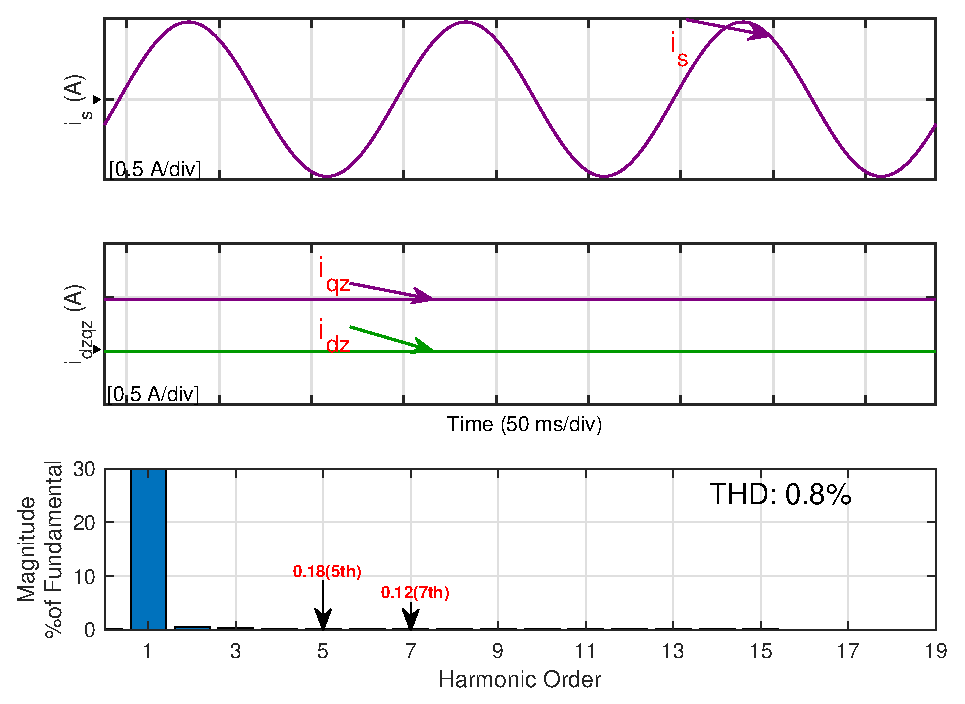
\includegraphics[width=\linewidth]{./MidSpeedLowLoadSteadyState}
    \caption{Low load: \(T=0.3~\mathrm{N\,m}\), \\THD \(=0.8\%\).}
    \label{fig:PIIdeal_1000rpm_low}
  \end{subfigure}\hfill
  \begin{subfigure}{0.485\textwidth}
    \centering
    % Replace with your exported plot/image
    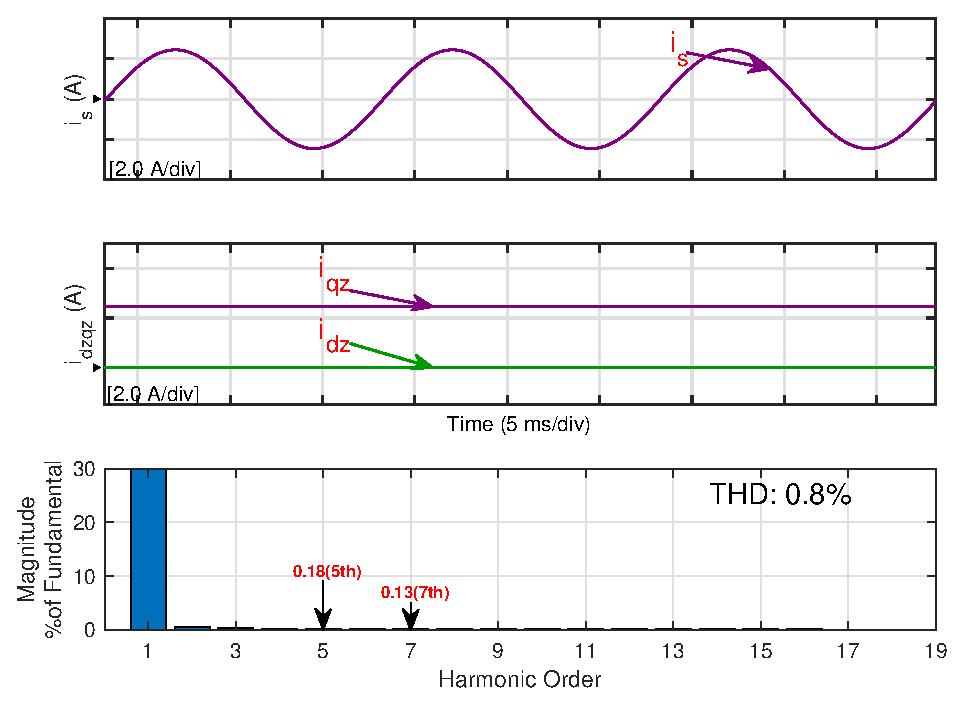
\includegraphics[width=\linewidth]{./MidSpeedMidLoadSteadyState}
    \caption{Medium load: \(T=1.75~\mathrm{N\,m}\),\\ THD \(=0.8\%\).}
    \label{fig:PIIdeal_1000rpm_med}
  \end{subfigure}
  \caption{PI controller steady state at 50\% rated speed (1000 rpm, ideal model). Each panel shows phase current, \(i_{dq}\), and THD.}
  \label{fig:PIIdeal_1000rpm}
\end{figure}


\subsection{Unbalanced Grid Operation}
With an ideal plant/inverter model (no non-linearities or disturbances), the sensorless PI drive maintains accurate low-speed control across load extremes. At 5\% of rated speed (100~rpm), the phase-current THD is \(\mathbf{1.3\%}\) at low load (10\% rated torque, \(0.3~\mathrm{N\!\cdot\!m}\)) and \(\mathbf{0.3\%}\) at high load (100\% rated torque, \(3.5~\mathrm{N\!\cdot\!m}\)); see Fig.~\ref{fig:PIIdeal_100rpm}. At 10\% of rated speed (200~rpm), the THD is \(\mathbf{1.6\%}\) at \(0.3~\mathrm{N\!\cdot\!m}\) and again \(\mathbf{0.3\%}\) at \(3.5~\mathrm{N\!\cdot\!m}\); see Fig.~\ref{fig:PIIdeal_200rpm}. In both tests the tracking is tight and ripple modest; the lower THD at higher load reflects stronger EMF/current improving the sensorless angle estimation and reducing relative harmonic content. Overall, these ideal-simulation results evidence robust PI performance at low speeds under all tested loads.

% Requires in preamble:
% \usepackage{graphicx}
% \usepackage{subcaption}
% (Optional) \usepackage{siunitx}

% ---------- Fig: PI at 5% rated (100 rpm) ----------
\begin{figure}[H]
  \centering
  \begin{subfigure}{0.485\textwidth}
    \centering
    % Replace with your exported plot/image
    
\includegraphics[width=\linewidth]{./PISteadyStateLowLoad100Rpm}
    \caption{Low load: \(T=0.3~\mathrm{N\,m}\), THD \(=1.3\%\).}
    \label{fig:PIIdeal_100rpm_low}
  \end{subfigure}\hfill
  \begin{subfigure}{0.485\textwidth}
    \centering
    % Replace with your exported plot/image
    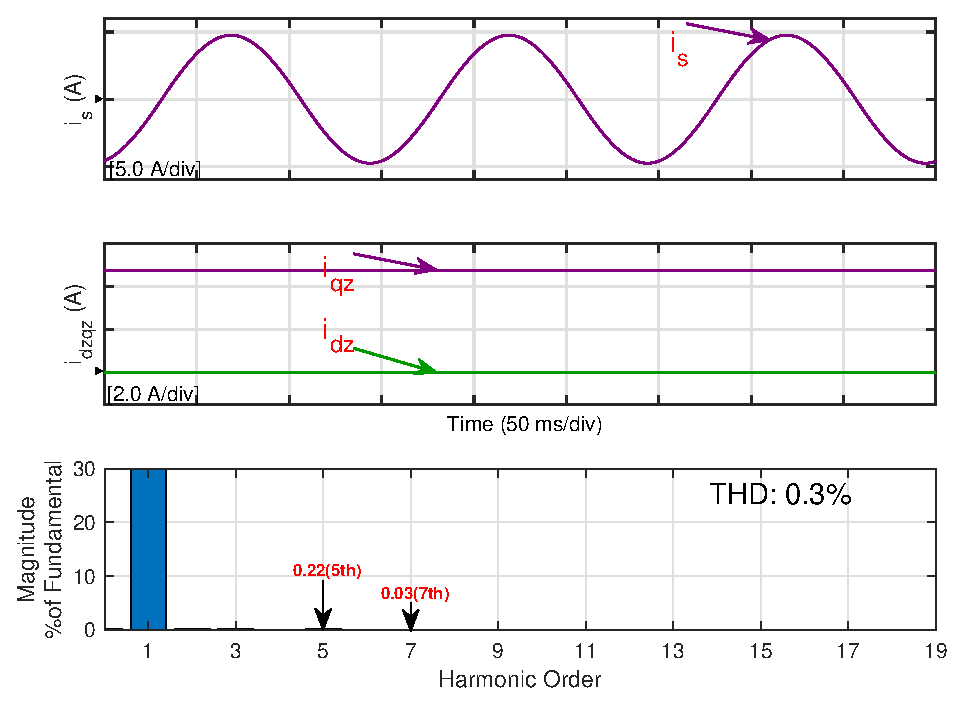
\includegraphics[width=\linewidth]{./PISteadyStateHighLoad100Rpm}
    \caption{High load: \(T=3.5~\mathrm{N\,m}\), THD \(=0.3\%\).}
    \label{fig:PIIdeal_100rpm_high}
  \end{subfigure}
  \caption{PI controller at 5\% rated speed (100 rpm, ideal model). Each panel shows phase current, \(i_{dq}\), and THD.}
  \label{fig:PIIdeal_100rpm}
\end{figure}

% ---------- Fig: PI at 10% rated (200 rpm) ----------
\begin{figure}[H]
  \centering
  \begin{subfigure}{0.485\textwidth}
    \centering
    % Replace with your exported plot/image
    
\includegraphics[width=\linewidth]{./PISteadyStateLowLoad200Rpm}
    \caption{Low load: \(T=0.3~\mathrm{N\,m}\), THD \(=1.6\%\).}
    \label{fig:PIIdeal_200rpm_low}
  \end{subfigure}\hfill
  \begin{subfigure}{0.485\textwidth}
    \centering
    % Replace with your exported plot/image
    
\includegraphics[width=\linewidth]{./PISteadyStateHighLoad200Rpm}
    \caption{High load: \(T=3.5~\mathrm{N\,m}\), THD \(=0.3\%\).}
    \label{fig:PIIdeal_200rpm_high}
  \end{subfigure}
  \caption{PI controller at 10\% rated speed (200 rpm, ideal model). As in the 100 rpm case, speed and currents remain well behaved; higher load yields lower relative harmonic content.}
  \label{fig:PIIdeal_200rpm}
\end{figure}

\subsection{Dynamic Performance}
Under an ideal plant/inverter (no non-linearities or disturbances), the PI speed loop tracks set-point changes within the 10–50\% band (100~rpm \(\rightarrow\) 1000~rpm) cleanly at both load extremes. At \emph{low load} (10\% rated torque, \(0.3~\mathrm{N\,m}\)), the measured speed follows the command with overshoot \(\mathbf{<10\%}\) and negligible steady-state error (see Fig.~\ref{fig:PIDyn_100to1000_low}). At \emph{rated load} (\(3.5~\mathrm{N\,m}\)), the response is slightly slower but remains well damped with overshoot \(\mathbf{<10\%}\) and zero steady-state error (see Fig.~\ref{fig:PIDyn_100to1000_rated}). These results confirm robust and smooth dynamic behavior across the tested range.

% Requires in preamble:
% \usepackage{graphicx}
% \usepackage{subcaption}

\begin{figure}[H]
  \centering
  \begin{subfigure}{0.485\textwidth}
    \centering
    % Replace with your exported plot/image
    
\includegraphics[width=\linewidth]{./DynamicResponsePILowLoad}
    \caption{Low load: \(T=0.3~\mathrm{N\,m}\). Overshoot \(<10\%\); zero steady-state error.}
    \label{fig:PIDyn_100to1000_low}
  \end{subfigure}\hfill
  \begin{subfigure}{0.485\textwidth}
    \centering
    % Replace with your exported plot/image
    
\includegraphics[width=\linewidth]{./DynamicResponsePIHighLoad}
    \caption{Rated load: \(T=3.5~\mathrm{N\,m}\). Slightly slower, well-damped; overshoot \(<10\%\).}
    \label{fig:PIDyn_100to1000_rated}
  \end{subfigure}
  \caption{PI controller dynamic response (ideal model) for speed changes within the \(10\%\!\to\!50\%\) rated band (100~rpm to 1000~rpm). Each panel shows command vs.\ speed, \(i_q\), and phase currents.}
  \label{fig:PIDyn_100to1000}
\end{figure}


\subsection{Parameter Variation}
In the ideal (noise-/nonlinearity-free) simulation, the PI controller was exercised with a deliberately biased motor model: \(R_s\) increased by \(+25\%\) and \(L_{d,q}\) decreased by \(25\%\). This shifts the electrical time constant from \(\tau=L/R\) to \(\tau'=\tfrac{0.75L}{1.25R}=0.60\,\tau\), moving the plant pole right and nudging the closed-loop cutoff upward while preserving phase margin. At the worst case examined—5\% rated speed (100~rpm)—the phase-current THD rises modestly from \(\mathbf{1.3\%}\) to \(\mathbf{1.7\%}\), but speed tracking and settling remain essentially unchanged. As illustrated in Fig.~\ref{fig:PIParameterVariation} (phase current, \(dq\) currents, and THD), the small THD increase reflects the altered crossover and slight model–controller mismatch; with no inverter non-idealities or disturbances, there is no mechanism to amplify it, so PI performance stays robust.
% Requires in preamble:
% \usepackage{graphicx}
% \usepackage{subcaption}

\begin{figure}[H]
  \centering
  
\includegraphics[width=0.485\linewidth]{./ParameterVariation}
  \caption{PI controller—parameter variation at 5\% rated speed (100 rpm, ideal model). The motor model is perturbed with \(R_s{+}25\%\) and \(L_{d,q}{-}25\%\). Panels show (a) phase current overlay, (b) \(dq\) currents, and (c) THD comparison.}
  \label{fig:PIParameterVariation}
\end{figure}



\subsection{Load Variation}
At 1000 rpm, the torque load was swept from 10\% to 100\% of rated in 20\% increments, each plateau held to steady state. As shown in Fig.~\ref{fig:PILoadVariation}, the PI loop maintains the commanded speed with small, well-damped transients at each step; \(i_q\) increases in clean steps to furnish torque and the phase currents scale proportionally without oscillation. Figure~\ref{fig:PILoadVariation} thus evidences robust disturbance rejection and steady regulation across the entire load range under ideal conditions.

% Requires in preamble:
% \usepackage{graphicx}
% \usepackage{subcaption}

\begin{figure}[H]
  \centering
  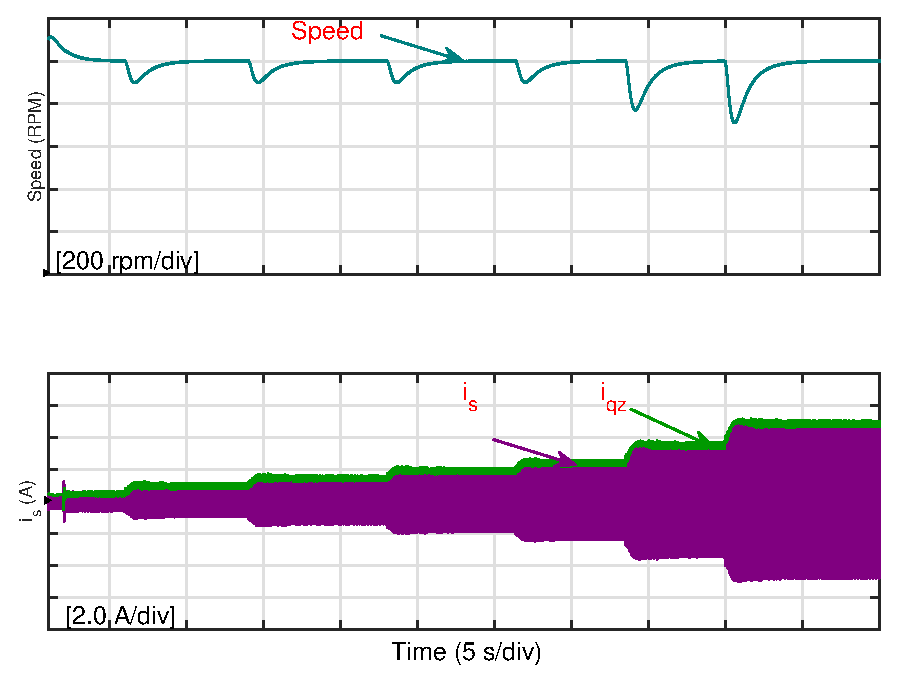
\includegraphics[width=0.6\linewidth]{./LoadVariation}
  \caption{PI controller under load variation at 50\% rated speed (1000 rpm, ideal model). The load torque steps from 10\% to 100\% in 20\% increments.}
  \label{fig:PILoadVariation}
\end{figure}

% =====================================================================
% Subsection: Motor and Drive Parameters (Comprehensive Table)
% Requires in preamble: \usepackage{longtable,booktabs}
% Optional: \usepackage{siunitx} for neat units
% =====================================================================



% End of subsection




% Notes: choose f_{T,min} just above current-loop BW; f_{C,min} above PLL natural freq;
% use Tustin discretization; update states when cutoffs change to avoid transients.



% ---- Example BibTeX keys (replace with your .bib entries) ----
% @book{Krause2013, title={Analysis of Electric Machinery and Drive Systems}, author={Krause, P. C. and Wasynczuk, O. and Sudhoff, S. D.}, year={2013}, publisher={Wiley}}
% @book{Leonhard2001, title={Control of Electrical Drives}, author={Leonhard, W.}, year={2001}, publisher={Springer}}
% @book{Vas1998, title={Sensorless Vector and Direct Torque Control}, author={Vas, P.}, year={1998}, publisher={Oxford}}


\chapter{Model Predictive Control in Motor Drives} \label{chap:mpc}
\graphicspath{{./Chapters/CH3/Pictures/}}
\let\cleardoublepage\clearpage

\section{Overview and Categorization}
\subsection{Overview}
\label{subsec:mpc-overview}

Model predictive control (MPC) brings a simple promise to power electronics: decide the next switching action by looking one step into the future and choosing the option that best serves the objectives. Unlike classical controllers that shape dynamics indirectly through gains and bandwidths, MPC works with an explicit model of the converter–machine pair and a concrete statement of what “good” means—tracking accuracy, modest switching activity, bounded voltages and currents, and respect for hardware limits. In a drive inverter these choices must be made at microsecond time scales; the plant is hybrid (continuous currents driven by discrete switch positions), the actuation is constrained (finite switching states and a limited voltage polygon), and nonidealities such as dead time and device drops lightly bend the physics. MPC fits this geometry naturally.

At each sampling instant the controller predicts what the electrical variables will do under a set of candidate actions, evaluates a cost for each candidate, and applies the one with the smallest cost. When the candidate set is the finite collection of inverter switching states, the controller decides which vector to apply next; when the decision is a continuous voltage or duty vector, the controller computes an optimal value and then realizes it with modulation. In both cases the essential ingredients are the same: a discrete-time prediction model, a cost function that encodes the priorities of the application, explicit constraints, and an implementation that closes the loop deterministically within the sampling budget. This chapter organizes those ingredients for power-electronics systems and sets the stage for the motor-drive controller designed later.

\subsection{Categorization of MPC Approaches}

There are two principal MPC flavors in power converters.
FCS-MPC treats the inverter as a device with a small catalogue of admissible switching vectors. The controller evaluates all admissible vectors over a short horizon—often a single step—and chooses the one that best advances the target. The advantages are conceptual simplicity, direct handling of discrete actuation, and constant computational cost; the tradeoff is higher current ripple unless special measures (virtual vectors, horizon extension, or switching penalties) are employed.
Continuous-control-set MPC optimizes a continuous voltage (or duty) command using the prediction model and then realizes that command with a modulator such as space-vector PWM. The benefit is low ripple and direct access to classical constraints on voltages and currents; the tradeoff is a small layer of modulation logic and, in general, slightly higher computational burden.

In motor drives, the most common targets are the stator currents or the electromagnetic torque; flux and power are also used in special cases. Current-tracking MPC provides a natural inner loop; torque-tracking MPC absorbs the current-to-torque mapping into the prediction model and cost, which can simplify the outer speed loop. DC-link voltage or grid current tracking dominate in rectifiers and active front ends.

Most drive applications use a one-step horizon with delay compensation, which aligns with tight sampling budgets and yields dead-beat-like behavior. Two-step horizons can reduce ripple or incorporate switching frequency penalties more gracefully. In all cases, the timing model—sample, compute, and apply—must be explicit so that the prediction lands at the instant when the action actually appears at the machine terminals.

Linear models in stationary or synchronous frames are customary and sufficient for fast inner loops. Nonidealities (dead time, device drops, computation and ADC delays, saturation of the voltage vector) are often included through additive biases, effective voltage reduction, or explicit constraints in the cost. Where parameter drift is expected (for example, resistance with temperature), adaptive updates or observer-based estimates can be incorporated without changing the controller’s structure.


The cost function is the language in which priorities are expressed. A typical current-tracking term measures the error at the prediction instant; a switching-effort term discourages unnecessary transitions; soft constraints penalize excursions beyond the linear modulation region or current limits, while hard constraints clip decisions that are physically unreachable. Weighting can be normalized to physical units (volts, amperes, radians per second) to make tuning interpretable and portable across operating points.


In direct MPC the selected switching state is applied immediately by the gate driver. In M2PC a continuous reference voltage or duty vector is passed to an SVM block, which generates duty ratios while preserving the average voltage commanded by the optimizer. Both realizations can be embedded in the same framework; the choice is guided by ripple, efficiency, electromagnetic compatibility, and processor headroom.


This thesis adopts a formulation that is tailored to motor drives and their inverter non-idealities. The controller is expressed in the synchronous frame with a short prediction horizon, uses an average inverter model driven by space-vector duty cycles, and encodes both tracking accuracy and inverter limits in a compact cost. Nonidealities are represented within the prediction and decision layers rather than treated post-hoc, allowing the controller to anticipate and mitigate their effect. Subsequent sections develop the prediction model, the cost terms, and the real-time realization that make this possible.


% ==========================================================
% Section: Discrete-Time Models for Power Converters
% Requires: \usepackage{amsmath}
% ==========================================================


% ==========================================================
% Section: Finite-Control-Set MPC for a Two-Level Inverter
% Requires: \usepackage{amsmath,booktabs}
% ==========================================================

% ==========================================================
% Section: Finite-Control-Set MPC for a Two-Level Inverter
% (Detailed and simplified narrative, step-by-step)
% Requires: \usepackage{amsmath}
% ==========================================================

% ==========================================================
% Section: Finite-Control-Set MPC for a Two-Level Inverter
% (Explained as a method, step-by-step)
% Requires: \usepackage{amsmath}
% ==========================================================

% ==========================================================
% Finite-Control-Set MPC (with in-text figure references)
% Requires: \usepackage{amsmath,graphicx}
% ==========================================================

% -------- Figures placed near the discussion; LaTeX will float them --------

\section{Finite-Control-Set MPC for a Two-Level Inverter}
\label{sec:fcsmpc}

\subsection{Methodology}
Every sampling period, the inverter must output exactly one switching state. The idea of FCS–MPC is simple: we list the few admissible states, we predict what the motor currents would look like if we applied each one, we score those predictions with a small cost, and we choose the state with the lowest score. No duty computation and no PWM are required in the pure form as shown in Figure~\ref{fig:fcs-diagram}.

\begin{figure}[H]
  \centering
  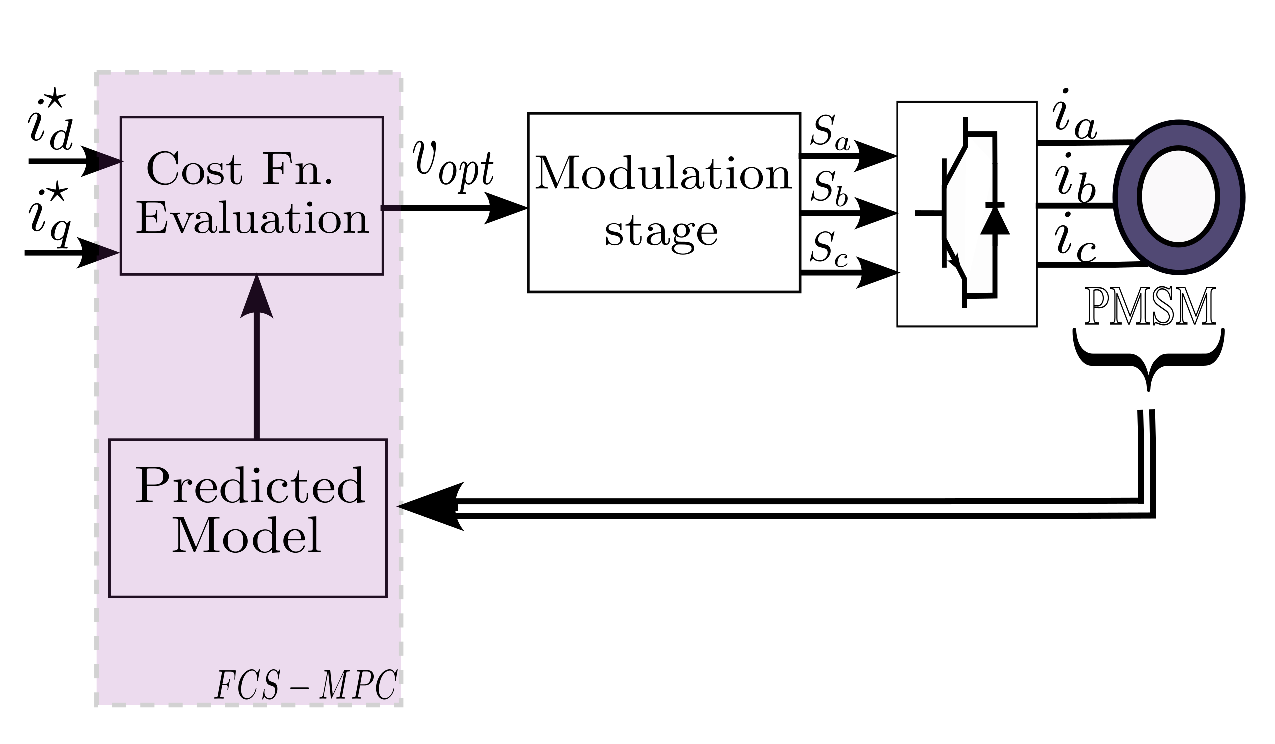
\includegraphics[width=\linewidth]{FCS}
  \caption{Control schematic for the FCS–MPC drive.}
  \label{fig:fcs-diagram}
\end{figure}


At the start of the control loop we have the measured/estimated currents, the electrical angle and speed, the DC-bus voltage, and the switching state that is currently being applied (from the previous decision). We also have the current references that we want to track at the prediction instant.
\begin{equation}
\label{eq:fcs-known}
\mathbf i[k]=\begin{bmatrix}i_d[k]\\ i_q[k]\end{bmatrix},\quad
\theta_e[k],\ \omega_e[k],\ V_{\mathrm{dc}}[k],\ \mathbf S[k{-}1], \mathbf i^{\ast}[k{+}2]
\end{equation}


Each inverter leg is either low ($0$) or high ($1$):
\begin{equation}
\label{eq:fcs-S}
\mathbf S=\begin{bmatrix}S_a\\ S_b\\ S_c\end{bmatrix}\in\{0,1\}^3 .
\end{equation}
There are six active states and two zero states as shown in Figure \ref{fig:InverterStates}. We usually test the six active states and optionally the zeros at very low speed or during limiting.

\begin{figure}[h]
	\centering
	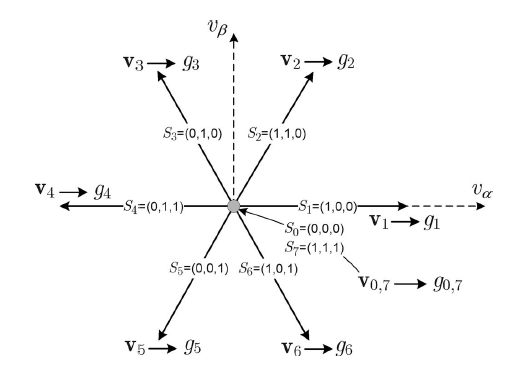
\includegraphics[width=\textwidth]{./InverterStates}
	\caption{Two Level Inverter Switching States}
	\label{fig:InverterStates}
\end{figure}

Given a candidate $\mathbf S_{i}$, we compute its stationary-frame voltages with two short formulas. First remove common mode and apply the Clarke map (written here in closed form):
\begin{equation}
\label{eq:fcs-valpha}
v_\alpha(\mathbf S_{i}) \;=\; V_{\mathrm{dc}}\!\left(\tfrac{2}{3}S^{i}_a-\tfrac{1}{3}S^{i}_b-\tfrac{1}{3}S^{i}_c\right),
\end{equation}
\begin{equation}
\label{eq:fcs-vbeta}
v_\beta(\mathbf S_{i}) \;=\; \frac{V_{\mathrm{dc}}}{\sqrt{3}}\,(S^{i}_b-S^{i}_c).
\end{equation}
We then rotate to the synchronous frame at the current electrical angle:
\begin{equation}
\label{eq:fcs-vdq}
\begin{bmatrix} v_d(\mathbf S_{i}) \\[2pt] v_q(\mathbf S_{i}) \end{bmatrix}
=
\begin{bmatrix}
\cos\theta_e[k] & \sin\theta_e[k]\\[2pt]
-\sin\theta_e[k] & \cos\theta_e[k]
\end{bmatrix}
\begin{bmatrix} v_\alpha(\mathbf S_{i}) \\[2pt] v_\beta(\mathbf S_{i}) \end{bmatrix}.
\end{equation}

We use the SPMSM electrical model in $dq$ and a one-step (or two-step) forward–Euler update. The continuous-time model is
\begin{equation}
\label{eq:fcs-ct}
\begin{bmatrix}\dot i_d\\[2pt]\dot i_q\end{bmatrix}
=
\frac{1}{L_s}
\begin{bmatrix}
- R_s & \ \ \ \omega_e L_s\\[2pt]
- \omega_e L_s & - R_s
\end{bmatrix}
\begin{bmatrix} i_d\\[2pt] i_q\end{bmatrix}
+
\frac{1}{L_s}\begin{bmatrix} v_d\\[2pt] v_q\end{bmatrix}
+
\frac{1}{L_s}\begin{bmatrix} 0\\[2pt] -\omega_e \lambda_f\end{bmatrix}.
\end{equation}
Freezing coefficients at time $k$, the one-step prediction under $\mathbf S$ is
\begin{equation}
\label{eq:fcs-euler}
\hat{\mathbf i}[k{+}1 ]
= \mathbf i[k]
+\frac{T_s}{L_s}\!\left(
\begin{bmatrix}
- R_s & \ \ \ \omega_e[k] L_s\\[2pt]
- \omega_e[k] L_s & - R_s
\end{bmatrix}\!\mathbf i[k]
+\begin{bmatrix} v_d(\mathbf S[k-1])\\[2pt] v_q(\mathbf S[k-1])\end{bmatrix}
+\begin{bmatrix} 0\\[2pt] -\omega_e[k]\lambda_f\end{bmatrix}
\right)\!.
\end{equation}
We first advance one step using the \emph{previous} state, then advance a second step with the \emph{candidate} state:
\begin{equation}
\label{eq:fcs-delay-1}
\hat{\mathbf i}[k{+}1]=\text{\eqref{eq:fcs-euler} evaluated with }\mathbf S[k{-}1],
\end{equation}
\begin{equation}
\label{eq:fcs-delay-2}
\hat{\mathbf i}^{i}[k{+}2]=\hat{\mathbf i}[k{+}1]
+\frac{T_s}{L_s}\!\left(
\begin{bmatrix}
- R_s & \ \ \ \omega_e[k] L_s\\[2pt]
- \omega_e[k] L_s & - R_s
\end{bmatrix}\!\hat{\mathbf i}[k{+}1]
+\begin{bmatrix} v_d(\mathbf S_{i})\\[2pt] v_q(\mathbf S_{i})\end{bmatrix}
+\begin{bmatrix} 0\\[2pt] -\omega_e[k]\lambda_f\end{bmatrix}
\right)\!.
\end{equation}
We compare \eqref{eq:fcs-euler} to a $k{+}1$ reference when there is no delay, and \eqref{eq:fcs-delay-2} to a $k{+}2$ reference when there is a one-sample delay.


The cost has a tracking term (normalized so tuning is consistent) and, optionally, a switching penalty to limit toggles. The tracking term is
\begin{equation}
\label{eq:fcs-Ji}
J_i(\mathbf S_{i}) \;=\; \big\| \mathbf W_i \big(\mathbf i^{\ast}[k{+}2]-\hat{\mathbf i^{i}}[k{+}2 ]\big) \big\|_2^2,
\end{equation}
with a simple diagonal normalizer
\begin{equation}
\label{eq:fcs-Wi}
\mathbf W_i=\mathrm{diag}\!\Big(\frac{1}{I_d^{\mathrm n}},\,\frac{1}{I_q^{\mathrm n}}\Big).
\end{equation}
The switching effort is penalized by counting how many legs would change:
\begin{equation}
\label{eq:fcs-Jdu}
J_{\Delta u}(\mathbf S_{i})=\lambda_{\Delta u}\,\big\|\mathbf S_{i}[k]-\mathbf S[k-1]\big\|_1,
\end{equation}
and the total cost is
\begin{equation}
\label{eq:fcs-J}
J_{i}=J_i(\mathbf S_{i})+J_{\Delta u}(\mathbf S_{i}).
\end{equation}

We choose the state with the smallest cost and hand it to the gate driver:
\begin{equation}
\label{eq:fcs-argmin}
\mathbf S^\star[k] \;=\; \arg\min_{\mathbf S\in\{0,1\}^3} J_{i}.
\end{equation}


\subsection{Algorithm Summary}
% FCS-MPCC in dq-frame — Summarized Steps (paste-ready)
\begin{enumerate}
  \item Define controller data: \(T_s\), machine/inverter parameters, limits, weights, and delay/dead-time compensation settings.
  \item Acquire signals each \(T_s\): \(i_d,i_q\), \(\theta_e,\omega_e\), \(V_{dc}\) (and any estimator outputs).
  \item Set references from outer loops: \(i_d^\star, i_q^\star\); apply saturation and rate limits.
  \item Enumerate feasible inverter switching states (e.g., 8 for a 2-level VSI).
  \item For each candidate state: compute its stator voltage vector, apply dead-time/device-drop compensation, and transform to the \(dq\) frame using \(\theta_e(k)\).
  \item Predict next-step \(i_d,i_q\) for each candidate using the discrete PMSM model (include one-step delay compensation; optionally use a two-step horizon).
  \item Evaluate a cost for each candidate:
        primary term = current-tracking error w.r.t. \(i_d^\star,i_q^\star\), and the switching effort;.
  \item Enforce constraints and discard infeasible candidates (current/voltage/thermal/speed).
  \item Select the candidate with minimum cost..
  \item Apply the selected switching state for the next control period.
  \item Update observers/estimators and any parameter adaptation; refresh \(\theta_e,\omega_e\); repeat each \(T_s\).
\end{enumerate}


\subsection{Modeling and Simulations}
This section validates the complete drive model and controllers through a focused suite of studies: (i) steady-state operation to verify ripple, losses, and harmonic content; (ii) low-speed operation to probe back-EMF limits and non-idealities; (iii)  dynamic performance under speed/current steps; (iv) parameter variation to gauge robustness against model mismatch; and (v) load variation to assess torque disturbance rejection.
\subsubsection{Steady State Operation}
At 1000 rpm (50\% rated) and 50\% rated load (\(1.75~\mathrm{N\,m}\)), the finite–control–set MPC produces the correct average torque but exhibits a phase–current THD of 8\% (see Fig.~\ref{fig:FCSIdeal_1000rpm_med}). This is characteristic of FCS applying a single vector per sample and frequently toggling between adjacent active vectors, which creates a staircase voltage, larger current ripple, and visible torque pulsations—even in the absence of non-idealities—yielding only moderate steady-state quality.

% Requires in preamble:
% \usepackage{graphicx}
% \usepackage{subcaption}

\begin{figure}[H]
  \centering
  
\includegraphics[width=0.7\linewidth]{./FCSMidSpeedMidLoadSteadyState}
  \caption{FCS–MPC steady state at 50\% rated speed (1000 rpm) and 50\% rated load (\(1.75~\mathrm{N\,m}\), ideal model). Panels show (a) phase current, (b) \(dq\) currents, and (c) THD (\(8\%\)).}
  \label{fig:FCSIdeal_1000rpm_med}
\end{figure}

\subsubsection{Low Speed Operation}
At 100 rpm (5\% rated) with an ideal inverter, the FCS controller applies a single active vector per sample; at \emph{low load} (10\% rated, \(0.3~\mathrm{N\,m}\)) the commanded stator voltage is tiny relative to the nearest active vector, so hexagon quantization is coarse and the staircase phase voltage yields 32\% THD (see Fig.~\ref{fig:FCSIdeal_100rpm_low}). At \emph{rated load} (\(3.5~\mathrm{N\,m}\)), the average voltage grows, the relative vector mismatch shrinks, and THD drops to 4\% (see Fig.~\ref{fig:FCSIdeal_100rpm_high}). Even under ideal conditions this remains above the PI baseline at 100 rpm (\(\mathbf{1.3\%}\) THD; Fig.~\ref{fig:PIIdeal_100rpm}), highlighting FCS’s intrinsic steady-state penalty at low-voltage operating points despite correct average torque.

\begin{figure}[H]
  \centering
  \begin{subfigure}{0.485\textwidth}
    \centering
    % Replace with your exported plot/image
    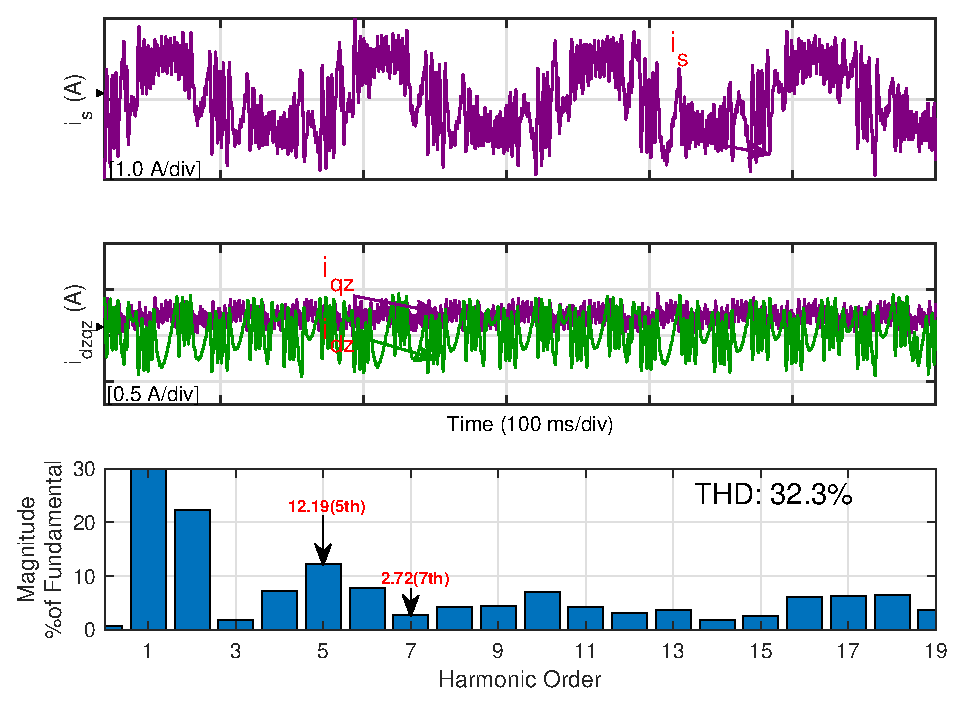
\includegraphics[width=\linewidth]{./FCSSteadyStateLowLoad100Rpm}
    \caption{Low load: \(T=0.3~\mathrm{N\,m}\), THD \(=32\%\).}
    \label{fig:FCSIdeal_100rpm_low}
  \end{subfigure}\hfill
  \begin{subfigure}{0.485\textwidth}
    \centering
    % Replace with your exported plot/image
    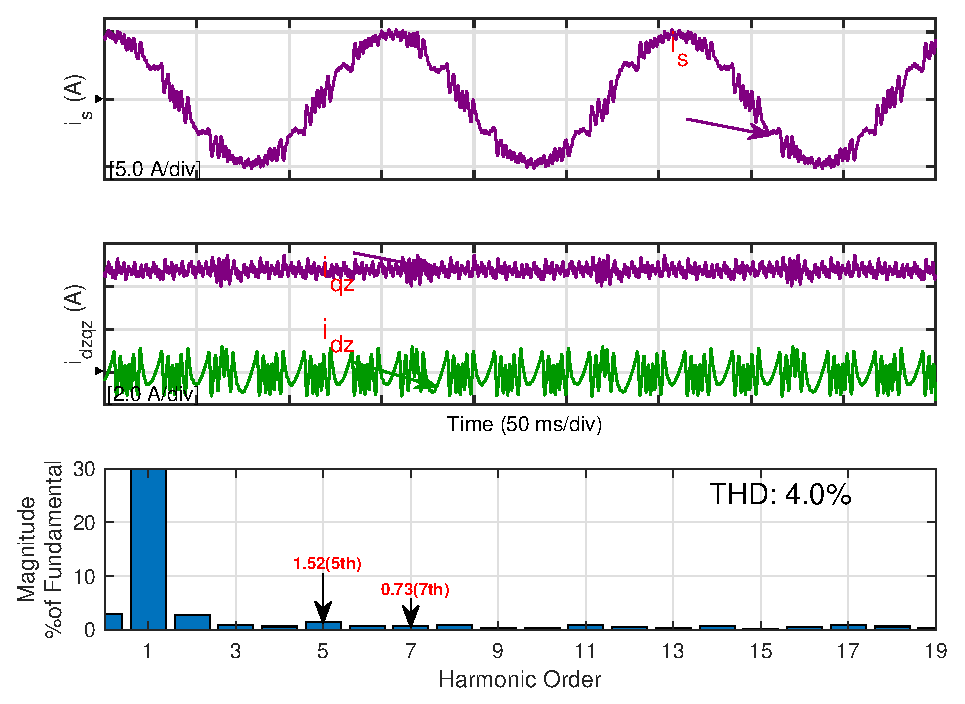
\includegraphics[width=\linewidth]{./FCSSteadyStateHighLoad100Rpm}
    \caption{Rated load: \(T=3.5~\mathrm{N\,m}\), THD \(=4\%\).}
    \label{fig:FCSIdeal_100rpm_high}
  \end{subfigure}
  \caption{FCS–MPC at low speed (100 rpm, ideal model). Each panel reports phase current, \(i_{dq}\), and THD; the low–load case shows coarse vector quantization and high ripple, while the rated–load case exhibits reduced mismatch and lower THD.}
  \label{fig:FCSIdeal_100rpm}
\end{figure}

\subsubsection{Dynamic Performance}
With an ideal plant/inverter (no non-linearities or disturbances), the FCS controller tracks speed commands within the 10–50\% band (100~rpm \(\rightarrow\) 1000~rpm) at both load extremes without failure or steady-state deviation. At low load (\(0.3~\mathrm{N\,m}\)), Fig.~\ref{fig:FCSDyn_100to1000_low} shows correct tracking but overshoot \emph{exceeds} \(10\%\) and \(i_q\)/phase currents carry pronounced ripple; at rated load (\(3.5~\mathrm{N\,m}\)), Fig.~\ref{fig:FCSDyn_100to1000_rated} exhibits similar behavior with slightly slower damping. This stems from FCS’s single-vector actuation: during transients it toggles between adjacent vectors, producing a staircase voltage that amplifies current ripple and torque pulsations compared to the PI benchmark.
% Requires in preamble:
% \usepackage{graphicx}
% \usepackage{subcaption}

\begin{figure}[H]
  \centering
  % --- (a) Low load ---
  \begin{subfigure}{0.485\textwidth}
    \centering
    % Replace with your exported plot/image
    
\includegraphics[width=\linewidth]{./FCSDynamicResponseLowLoad}
    \caption{Low load: \(T=0.3~\mathrm{N\,m}\). Overshoot \(>10\%\); pronounced \(i_q\)/phase-current ripple.}
    \label{fig:FCSDyn_100to1000_low}
  \end{subfigure}\hfill
  % --- (b) Rated load ---
  \begin{subfigure}{0.485\textwidth}
    \centering
    % Replace with your exported plot/image
    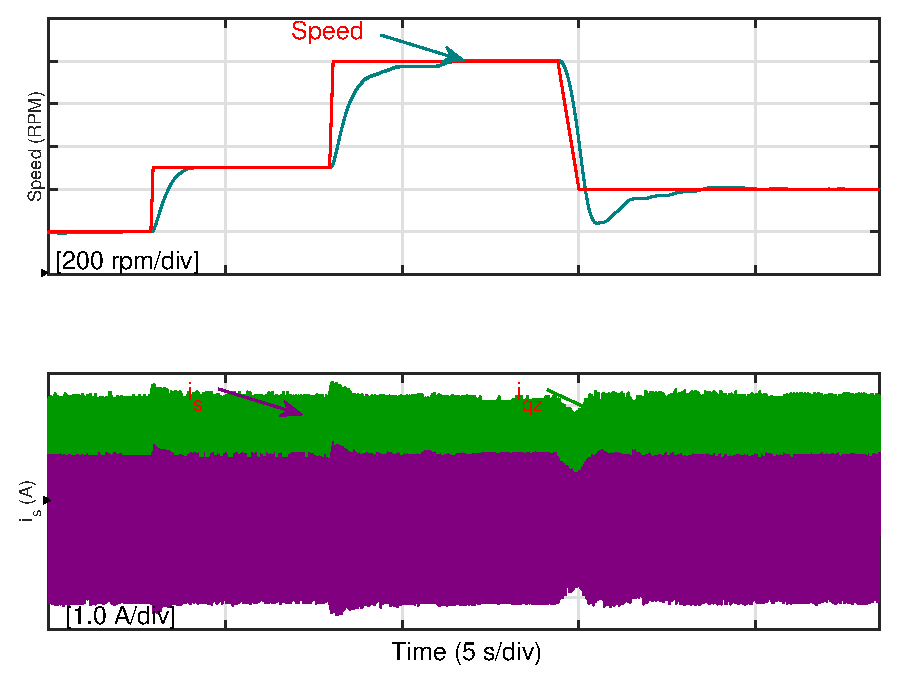
\includegraphics[width=\linewidth]{./FCSDynamicResponseHighLoad}
    \caption{Rated load: \(T=3.5~\mathrm{N\,m}\). Correct tracking, overshoot \(>10\%\); slightly slower damping.}
    \label{fig:FCSDyn_100to1000_rated}
  \end{subfigure}

  \caption{FCS–MPC dynamic response (ideal model) for speed changes within the \(10\%\!\to\!50\%\) rated band (100~rpm to 1000~rpm). Panels report command vs.\ speed, \(i_q\), and phase currents for (a) low load and (b) rated load.}
  \label{fig:FCSDyn_100to1000}
\end{figure}


\subsubsection{Parameter Variation}
To stress the prediction stage, the FCS controller was run with a deliberately biased internal model—stator resistance increased by \(+25\%\) and inductances decreased by \(25\%\)—while the plant and inverter remained ideal and the operating point was the worst case of 100 rpm (5\% rated). Under this mismatch the phase-current THD rose from \(\mathbf{32\%}\) (nominal model) to \(\mathbf{41\%}\). The degradation is expected: FCS ranks a single inverter vector per sample using one-step current predictions; errors in \(R_s\) and \(L\) bias those predictions, leading to suboptimal vector choices and coarser effective quantization on the hexagon. The result is amplified current harmonics and torque ripple—even without any non-idealities or disturbances—highlighting the sensitivity of FCS to prediction-model fidelity at low-voltage operating points.
% Requires in preamble:
% \usepackage{graphicx}

\begin{figure}[H]
  \centering
  % Replace with your exported composite plot (phase currents, dq currents, and THD)
  
\includegraphics[width=0.7\linewidth]{./FCSParameterVariation}
  \caption{FCS–MPC parameter variation at low speed (100 rpm, ideal model). The prediction model uses \(R_s{+}25\%\) and \(L_{d,q}{-}25\%\). The composite plot shows (left) phase currents with enhanced ripple, (middle) \(d\)- and \(q\)-axis currents, and (right) THD comparison—rising from \(\mathbf{32\%}\) (nominal model) to \(\mathbf{41\%}\) (biased model) due to suboptimal vector selection from prediction errors.}
  \label{fig:FCSParamVariation}
\end{figure}

\subsubsection{Load Variation}
At 1000 rpm, the load torque was stepped from 10\% to 100\% of rated in 20\% increments, each plateau held to steady state. As shown in Fig.~\ref{fig:FCSLoadVariation}, the commanded speed is maintained without droop; Fig.~\ref{fig:FCSLoadVariation} shows \(i_q\) rising in clean steps to furnish the added torque; and Fig.~\ref{fig:FCSLoadVariation} reports the phase currents with the characteristic FCS staircase ripple—transients remain well damped, confirming robust regulation under load changes.

\begin{figure}[H]
  \centering
  % Replace with your exported composite plot that contains
  % (left) speed response, (middle) dq-currents, (right) phase currents
  
\includegraphics[width=0.6\linewidth]{./FCSLoadVariation}
  \caption{FCS–MPC under load variation at 50\% rated speed (1000 rpm, ideal model).
  The composite figure shows the speed response (measured), \(q\)-axis currents, and the phase currents during torque steps from 10\% to 100\% of rated in 20\% increments.}
  \label{fig:FCSLoadVariation}
\end{figure}

% ==========================================================
% Section: Continuous-Control-Set MPC (CCS-MPC) with Modulation
% Requires: \usepackage{amsmath,booktabs}
% ==========================================================

% ==========================================================
% Section: Modulated Model Predictive Control (MMPC) with SVM
% Requires: \usepackage{amsmath,graphicx}
% ==========================================================

% ==========================================================
% Section: Modulated Model Predictive Control (M2PC) with SVM
% (Forward–Euler discretization; detailed derivation)
% Requires: \usepackage{amsmath,graphicx}
% ==========================================================

% ==========================================================
% Modulated Model Predictive Control (Forward–Euler, story form)
% Requires: \usepackage{amsmath,graphicx}
% ==========================================================

\section{Modulated Model Predictive Control}
\label{sec:mmpc}

\subsection{Methodology}
The rationale for moving beyond FCS–MPC (Sec.~\ref{sec:fcsmpc}) is straightforward. Applying a single active vector per period makes the switching frequency state-dependent and pushes actuation to the hexagon edges, which increases current ripple, spreads the spectrum, and forces heuristic switching-penalty tuning. The modulated predictive controller adopted here preserves the same one-step, model-based “look ahead and choose” idea, but it optimizes a continuous average voltage that is realized by space–vector modulation (SVM). Practically, at each sampling instant we evaluate what would happen if each inverter vector were applied over the next period, select the two adjacent active vectors that best reduce the current error, and compute their dwell times (plus a zero vector) so that the average current error over the period is driven to zero. The outcome is a fixed switching frequency by construction, reduced ripple and acoustic noise, an explicit voltage-feasibility check, and a clean path to include non-idealities as effective voltage biases. In this work, the electrical prediction uses a Forward–Euler discretization for simplicity and deterministic real-time load.

\begin{figure}[H]
  \centering
  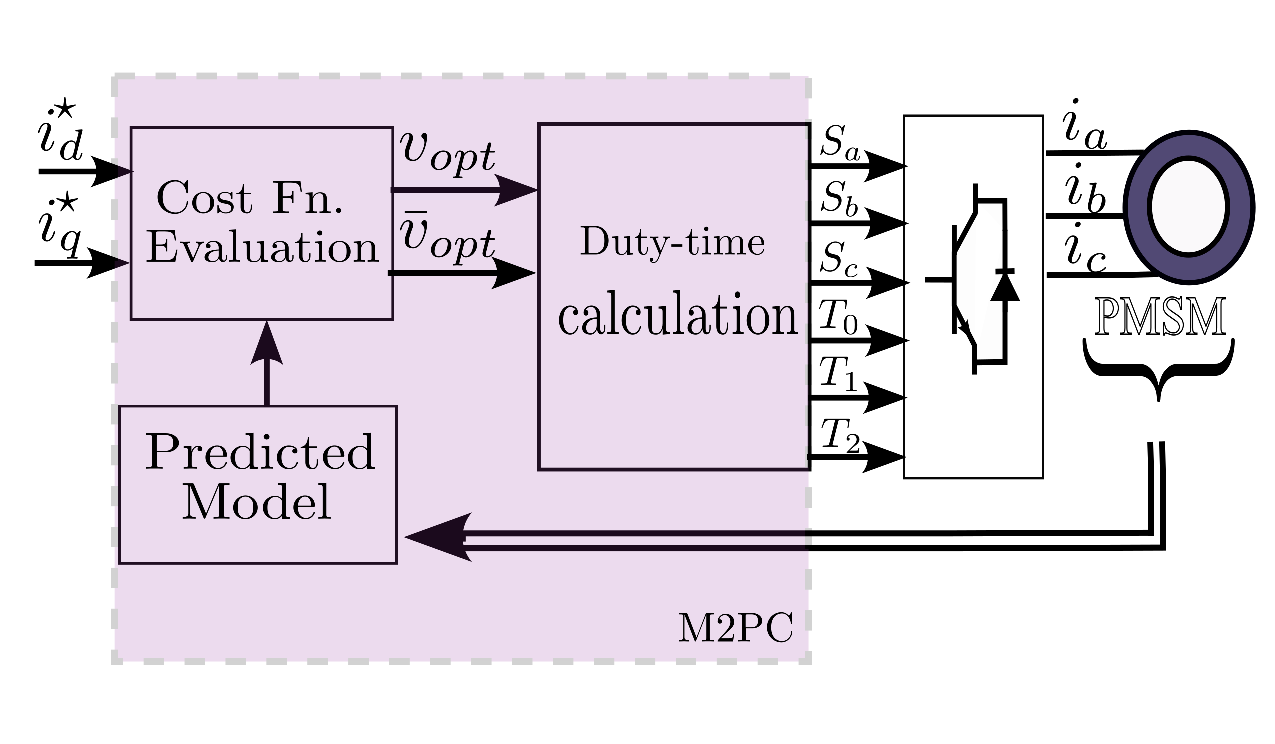
\includegraphics[width=\linewidth]{M2PC}
  \caption{Control schematic for the Modulated Model Predictive Controller Drive.}
  \label{fig:m2pc-diagram}
\end{figure}

The story begins by mapping each switching state into a stationary voltage vector. For a two-level inverter with state $\mathbf S=[S_a\ S_b\ S_c]^T\in\{0,1\}^3$ and dc bus $V_{\mathrm{dc}}$, the stationary components follow
\begin{equation}
\label{eq:m2pc-valphabeta}
v_\alpha(\mathbf S)\;=\;V_{\mathrm{dc}}\!\left(\tfrac{2}{3}S_a-\tfrac{1}{3}S_b-\tfrac{1}{3}S_c\right),\qquad
v_\beta(\mathbf S)\;=\;\tfrac{V_{\mathrm{dc}}}{\sqrt{3}}\,(S_b-S_c).
\end{equation}
These are rotated into the synchronous frame using the present electrical angle:
\begin{equation}
\label{eq:m2pc-vdq}
\begin{bmatrix} v_d \\[2pt] v_q \end{bmatrix}
=
\begin{bmatrix}
\cos\theta_e[k] & \sin\theta_e[k]\\[2pt]
-\sin\theta_e[k] & \cos\theta_e[k]
\end{bmatrix}
\begin{bmatrix} v_\alpha \\[2pt] v_\beta \end{bmatrix}.
\end{equation}
We then predict where the currents would land one sample later if that vector were applied for the full period. For an SPMSM ($L_d=L_q=L_s$), freezing coefficients at $k$ and defining $\gamma=T_s/L_s$, the Forward–Euler one-step update is
\begin{equation}
\label{eq:m2pc-fe-vector}
\hat{\mathbf i^{i}}[k{+}1]
=
\mathbf i[k]
+\gamma\left(
\begin{bmatrix}
- R_s & \ \ \omega_e[k] L_s\\[2pt]
- \omega_e[k] L_s & - R_s
\end{bmatrix}\mathbf i[k]
+
\begin{bmatrix} v^{i}_d[k] \\[2pt] v^{i}_q[k] \end{bmatrix}
+
\begin{bmatrix} 0 \\[2pt] -\,\omega_e[k]\lambda_f \end{bmatrix}
\right),
\end{equation}
that is, componentwise,
\begin{align}
\label{eq:m2pc-fe-id}
\hat i_d^{i}[k{+}1] &= i_d[k] + \gamma\left(-R_s i_d[k] + \omega_e[k]L_s i_q[k] + v^{i}_d[k]\right),\\
\label{eq:m2pc-fe-iq}
\hat i_q^{i}[k{+}1] &= i_q[k] + \gamma\left(-\omega_e[k]L_s i_d[k] - R_s i_q[k] + v^{i}_q[k] - \omega_e[k]\lambda_f\right).
\end{align}
With these predictions in hand for every admissible vector, we form a simple ranking cost against the one-step current target. Let the desired currents at the prediction instant be
\begin{equation}
\label{eq:m2pc-target}
\mathbf i^{\ast}[k{+}1]=\begin{bmatrix} i_d^{\ast}[k{+}1]\\[2pt] i_q^{\ast}[k{+}1]\end{bmatrix}.
\end{equation}
For each $\mathbf S^{i}$, compute the errors and quadratic score
\begin{equation}
\label{eq:m2pc-rank}
E_d^{i}[k+1]=i_d^{\ast}[k{+}1]-\hat i^{i}_d[k+1],\qquad
E_q^{i}[k+1]=i_q^{\ast}[k{+}1]-\hat i^{i}_q[k+1],\\
J^{i}[k+1]=(E_d^{i}[k+1])^2+(E_q^{i}[k+1])^2.
\end{equation}
The best active vector $v_{\mathrm{opt}}$ minimizes $J$; the second-best $v'_{\mathrm{opt}}$ is its neighbor on the SVM hexagon (a geometric fact routinely observed in practice). Using only these two and a zero vector $v_0$, we synthesize an average voltage over the next period whose mean current error is zero in both axes. Let the dwell times be $\tau_0,\tau_1,\tau_2$ for $\{v_0,\,v_{\mathrm{opt}},\,v'_{\mathrm{opt}}\}$ with $\tau_0+\tau_1+\tau_2=T_s$. Enforcing zero average error yields the linear conditions
\begin{equation}
\label{eq:m2pc-avg-err}
\begin{bmatrix}
E_d(v_0) & E_d(v_{\mathrm{opt}}) & E_d(v'_{\mathrm{opt}})\\[2pt]
E_q(v_0) & E_q(v_{\mathrm{opt}}) & E_q(v'_{\mathrm{opt}})\\[2pt]
1 & 1 & 1
\end{bmatrix}
\begin{bmatrix}\tau_0\\[2pt]\tau_1\\[2pt]\tau_2\end{bmatrix}
=
\begin{bmatrix}0\\[2pt]0\\[2pt]T_s\end{bmatrix},
\end{equation}
whose closed-form solution in terms of the error components is
\begin{align}
\label{eq:m2pc-tau0}
\tau_0 &= \frac{T_s\big(E_d(v_{\mathrm{opt}})\,E_q(v'_{\mathrm{opt}})-E_d(v'_{\mathrm{opt}})\,E_q(v_{\mathrm{opt}})\big)}{D},\\[2pt]
\label{eq:m2pc-tau1}
\tau_1 &= \frac{T_s\big(E_d(v'_{\mathrm{opt}})\,E_q(v_0)-E_d(v_0)\,E_q(v'_{\mathrm{opt}})\big)}{D},\\[2pt]
\label{eq:m2pc-tau2}
\tau_2 &= \frac{T_s\big(E_d(v_0)\,E_q(v_{\mathrm{opt}})-E_d(v_{\mathrm{opt}})\,E_q(v_0)\big)}{D},
\end{align}
with common denominator
\begin{equation}
\label{eq:m2pc-D}
D \;=\;
E_d(v_0)\!\big(E_q(v_{\mathrm{opt}})-E_q(v'_{\mathrm{opt}})\big)
+E_d(v_{\mathrm{opt}})\!\big(E_q(v'_{\mathrm{opt}})-E_q(v_0)\big)
+E_d(v'_{\mathrm{opt}})\!\big(E_q(v_0)-E_q(v_{\mathrm{opt}})\big).
\end{equation}
When all three $\tau_j$ are nonnegative and sum to $T_s$, the origin lies in the triangle spanned by the error vectors $\{[E_d\ E_q]^T\}$, and the synthesized average is feasible inside the linear SVM region. If any $\tau_j<0$, a simple, robust fallback is to clip the negative time to zero, renormalize the remainder to $T_s$, or reselect the second vector from the adjacent sector.

The translation from dwell times to per-leg duty cycles is the usual centered SVM construction. If the sector ordering within the period is chosen in the standard way (zero–active–active–zero), the generic duty template reads
\begin{equation}
\label{eq:m2pc-duties}
\begin{bmatrix} d_{\mathrm{high}} \\[2pt] d_{\mathrm{mid}} \\[2pt] d_{\mathrm{low}} \end{bmatrix}
=
\frac{1}{T_s}
\begin{bmatrix}
\tau_1 + \tau_2 + \tfrac{1}{2}\tau_0 \\[4pt]
\tau_2 + \tfrac{1}{2}\tau_0 \\[4pt]
\tfrac{1}{2}\tau_0
\end{bmatrix},
\end{equation}
followed by the usual sector-dependent permutation into $[d_a\ d_b\ d_c]^T$. Feasibility in linear modulation corresponds to $\tau_j\in[0,T_s]$ and $\tau_0+\tau_1+\tau_2=T_s$, equivalently to the stationary average satisfying
\begin{equation}
\label{eq:m2pc-vlimit}
\sqrt{\big(\bar v_\alpha^\ast\big)^2+\big(\bar v_\beta^\ast\big)^2}\ \le\ \tfrac{1}{2}\,V_{\mathrm{dc}}.
\end{equation}


In summary, the modulated predictive controller evaluates the effect of all inverter vectors through the light Forward–Euler map \eqref{eq:m2pc-fe-vector}–\eqref{eq:m2pc-fe-iq}, ranks them against the one-step target \eqref{eq:m2pc-rank}, and replaces “apply one vector” with the SVM dwell synthesis \eqref{eq:m2pc-avg-err}–\eqref{eq:m2pc-duties}. The result is a fixed-frequency, low-ripple inner loop that remains fully model-based, integrates naturally with the observer and speed loop, and provides a fair baseline for later comparisons against PI–FOC and non-ideal inverter compensation.

\subsection{Algorithm Summary}
TBD 

\subsection{Modeling and Simulations}
This section validates the complete drive model and controllers through a focused suite of studies: (i) steady-state operation to verify ripple, losses, and harmonic content; (ii) low-speed operation to probe back-EMF limits and non-idealities; (iii)  dynamic performance under speed/current steps; (iv) parameter variation to gauge robustness against model mismatch; and (v) load variation to assess torque disturbance rejection.
\subsubsection{Steady State Operation}
With an ideal plant/inverter (no non-linearities or disturbances), the modulated MPC (SVM-based) holds 1000 rpm with very low harmonic content across loads: at low load (10\% rated torque, \(0.3~\mathrm{N\,m}\)) the phase-current THD is 0.4\% (see Fig.~\ref{fig:M2PCIdeal_1000rpm_low}), and at medium load (50\% rated torque, \(1.75~\mathrm{N\,m}\)) it is 0.7\% (see Fig.~\ref{fig:M2PCIdeal_1000rpm_med}). The improved spectral cleanliness stems from optimizing a continuous average voltage each sample and realizing it via SVM at fixed switching frequency, which suppresses staircase ripple. In this ideal setting the modulated MPC delivers robust steady-state operation with lower THD than PI at the same speed/load and far below FCS, while maintaining tight speed regulation.

\begin{figure}[H]
  \centering
  % --- (a) Low load ---
  \begin{subfigure}{0.485\textwidth}
    \centering
    % Replace with your exported plot/image
    
\includegraphics[width=\linewidth]{./MPCMidSpeedLowLoadSteadyState}
    \caption{Low load: \(T=0.3~\mathrm{N\,m}\),\\ THD \(=0.4\%\).}
    \label{fig:M2PCIdeal_1000rpm_low}
  \end{subfigure}\hfill
  % --- (b) Medium load ---
  \begin{subfigure}{0.485\textwidth}
    \centering
    % Replace with your exported plot/image
    
\includegraphics[width=\linewidth]{./MPCMidSpeedMidLoadSteadyState}
    \caption{Medium load: \(T=1.75~\mathrm{N\,m}\),\\ THD \(=0.7\%\).}
    \label{fig:M2PCIdeal_1000rpm_med}
  \end{subfigure}

  \caption{Modulated MPC (SVM-based) steady state at 50\% rated speed (1000 rpm, ideal model). Each panel shows phase currents, \(i_{dq}\), and THD. The modulated formulation yields very low harmonic content at both loads.}
  \label{fig:M2PCIdeal_1000rpm}
\end{figure}

\subsubsection{Low Speed Operation}
Under an ideal plant/inverter (no non-linearities or disturbances), the modulated MPC maintains accurate sensorless control at very low speeds. At 5\% rated (100~rpm), the phase-current THD is 0.3\% at low load (\(0.3~\mathrm{N\,m}\), see Fig.~\ref{fig:M2PCIdeal_100rpm_low}) and 0.4\% at rated load (\(3.5~\mathrm{N\,m}\), see Fig.~\ref{fig:M2PCIdeal_100rpm_high}); at 10\% rated (200~rpm), the THD is 0.5\% at low load (\(0.3~\mathrm{N\,m}\), see Fig.~\ref{fig:M2PCIdeal_200rpm_low}) and 0.1\% at rated load (\(3.5~\mathrm{N\,m}\), see Fig.~\ref{fig:M2PCIdeal_200rpm_high}). Across these cases the controller tracks with negligible steady-state error and fixed-frequency, SVM-based actuation that suppresses staircase ripple. Overall, the low-speed THD is comparable to or better than the PI baseline and far below FCS, evidencing robust performance under all tested loads in the absence of disturbances.
% Requires in preamble:
% \usepackage{graphicx}
% \usepackage{subcaption}

% ---------- MPC at 5% rated (100 rpm) ----------
\begin{figure}[t]
  \centering
  % Low load
  \begin{subfigure}{0.485\textwidth}
    \centering
    % Replace with your exported plot/image
    
\includegraphics[width=\linewidth]{./MPCSteadyStateLowLoad100Rpm}
    \caption{Low load: \(T=0.3~\mathrm{N\,m}\); THD \(=0.3\%\).}
    \label{fig:M2PCIdeal_100rpm_low}
  \end{subfigure}\hfill
  % Rated load
  \begin{subfigure}{0.485\textwidth}
    \centering
    % Replace with your exported plot/image
    
\includegraphics[width=\linewidth]{./MPCSteadyStateHighLoad100Rpm}
    \caption{Rated load: \(T=3.5~\mathrm{N\,m}\); THD \(=0.4\%\).}
    \label{fig:M2PCIdeal_100rpm_high}
  \end{subfigure}
  \caption{Modulated MPC (SVM-based) at 5\% rated speed (100 rpm, ideal model). Each panel shows phase currents, \(i_{dq}\), and THD.}
  \label{fig:M2PCIdeal_100rpm}
\end{figure}

% ---------- MPC at 10% rated (200 rpm) ----------
\begin{figure}[t]
  \centering
  % Low load
  \begin{subfigure}{0.485\textwidth}
    \centering
    % Replace with your exported plot/image
    
\includegraphics[width=\linewidth]{./MPCSteadyStateLowLoad200Rpm}
    \caption{Low load: \(T=0.3~\mathrm{N\,m}\); THD \(=0.5\%\).}
    \label{fig:M2PCIdeal_200rpm_low}
  \end{subfigure}\hfill
  % Rated load
  \begin{subfigure}{0.485\textwidth}
    \centering
    % Replace with your exported plot/image
    
\includegraphics[width=\linewidth]{./MPCSteadyStateHighLoad200Rpm}
    \caption{Rated load: \(T=3.5~\mathrm{N\,m}\); THD \(=0.1\%\).}
    \label{fig:M2PCIdeal_200rpm_high}
  \end{subfigure}
  \caption{Modulated MPC (SVM-based) at 10\% rated speed (200 rpm, ideal model). Each panel shows phase currents, \(i_{dq}\), and THD.}
  \label{fig:M2PCIdeal_200rpm}
\end{figure}

\subsubsection{Dynamic Performance}
With an ideal plant/inverter (no non-linearities or disturbances), the modulated MPC tracks speed commands within the 10–50\% band (100~rpm \(\rightarrow\) 1000~rpm) cleanly at both load extremes. At \emph{low load} (10\% rated, \(0.3~\mathrm{N\,m}\)), Fig.~\ref{fig:M2PCDyn_100to1000_low} shows overshoot \(\mathbf{<10\%}\) and negligible steady-state error; at rated load (\(3.5~\mathrm{N\,m}\)), Fig.~\ref{fig:M2PCDyn_100to1000_rated} exhibits similarly well-damped behavior with a modestly slower rise. In both cases, the SVM-realized average voltage yields markedly smoother \(i_q\)/phase currents—far lower torque ripple than FCS and noticeably lower than PI—confirming robust dynamic performance across the tested range.
% Requires in preamble:
% \usepackage{graphicx}
% \usepackage{subcaption}

\begin{figure}[t]
  \centering
  % --- (a) Low load ---
  \begin{subfigure}{0.485\textwidth}
    \centering
    % Replace with your exported plot/image
    
\includegraphics[width=\linewidth]{./MPCDynamicResponseLowLoad}
    \caption{Low load: \(T=0.3~\mathrm{N\,m}\). Overshoot \(<10\%\); negligible steady-state error; smooth \(i_q\)/phase currents.}
    \label{fig:M2PCDyn_100to1000_low}
  \end{subfigure}\hfill
  % --- (b) Rated load ---
  \begin{subfigure}{0.485\textwidth}
    \centering
    % Replace with your exported plot/image
    
\includegraphics[width=\linewidth]{./MPCDynamicResponseHighLoad}
    \caption{Rated load: \(T=3.5~\mathrm{N\,m}\). Overshoot \(<10\%\); slightly slower rise; very low torque ripple.}
    \label{fig:M2PCDyn_100to1000_rated}
  \end{subfigure}

  \caption{Modulated MPC (SVM-based) dynamic response (ideal model) for speed changes within the \(10\%\!\to\!50\%\) rated band (100~rpm to 1000~rpm). Each panel shows command vs.\ speed, \(i_q\), and phase currents. The modulated formulation yields markedly smoother currents and lower torque ripple than FCS and PI.}
  \label{fig:M2PCDyn_100to1000}
\end{figure}

\subsubsection{Parameter Variation}
At 5\% rated speed (100~rpm), using a biased prediction model (\(R_s{+}25\%\), \(L_{d,q}{-}25\%\)) leaves the modulated MPC’s steady-state quality unchanged: phase-current THD stays at 0.3\% (Fig.~\ref{fig:M2PCParamVariation}). The fixed-frequency, SVM-based actuation and per-sample voltage optimization make the controller largely insensitive to moderate \(R\!-\!L\) errors—more robust than PI (1.3\% \(\rightarrow\) 1.7\%) and far better than FCS (32\% \(\rightarrow\) 41\%).

% Requires in preamble:
% \usepackage{graphicx}

\begin{figure}[H]
  \centering
  % Replace with your exported composite plot (speed, dq currents, phase currents, THD)
  
\includegraphics[width=0.6\linewidth]{./MPCParameterVariation}
  \caption{Modulated MPC under parameter variation at 5\% rated speed (100 rpm, ideal model).
  The prediction model uses \(R_s{+}25\%\) and \(L_{d,q}{-}25\%\). The figure reports  phase currents, \(d\)- and \(q\)-axis currents, and the THD comparison, which remains at \(\mathbf{0.3\%}\)—indistinguishable from the no-variation case—indicating high robustness of bandwidth/cutoff and harmonic performance.}
  \label{fig:M2PCParamVariation}
\end{figure}

\subsubsection{Load Variation}
At 1000 rpm the load torque was stepped from 10\% to 100\% of rated in 20\% increments, each held to steady state. As shown in Fig.~\ref{fig:M2PCLoadVariation}, the modulated MPC maintains the commanded speed without droop; \(i_q\) increases in clean, proportional steps to furnish the added torque, and the phase currents remain smooth thanks to the fixed-frequency SVM realization of the optimized average voltage. Transients are well damped and steady-state ripple stays low throughout, evidencing robust disturbance rejection under load changes.
% Requires in preamble:
% \usepackage{graphicx}

\begin{figure}[H]
  \centering
  % Replace with your exported composite plot that contains
  % (left) speed response, (middle) dq-currents, (right) phase currents
  
\includegraphics[width=0.6\linewidth]{./MPCLoadVariation}
  \caption{Modulated MPC under load variation at 50\% rated speed (1000 rpm, ideal model).
  The composite figure shows motor speed, \(q\)-axis currents, and phase currents during torque steps from 10\% to 100\% of rated in 20\% increments.}
  \label{fig:M2PCLoadVariation}
\end{figure}

% bridge to proposed controller
 
\chapter{Non-idealities Modeling and Simulation} \label{chap:results}
\graphicspath{{./Chapters/CH4/Pictures/}}
\let\cleardoublepage\clearpage

\section{Overview}
\label{subsec:ch4-overview}

This chapter closes the gap between the ideal drive models used so far and the bench-realistic behavior observed on hardware. We proceed in two stages. First, we measure and identify the permanent-magnet synchronous motor (PMSM) parameters needed by analysis and control—stator resistance, synchronous inductances (or \(L_d,L_q\)), permanent-magnet flux linkage, pole pairs, and the mechanical pair \((J,B)\) with optional Coulomb friction. The emphasis is on practical, repeatable procedures that can be executed with readily available instrumentation (e.g., an RLC meter and the drive).

Second, we model the inverter’s non-ideal behavior and show how it alters the voltages actually seen by the machine. The focus is on effects that matter most in low-speed, high-precision operation: dead time, device conduction drops and on-state resistances, current-polarity–dependent commutation asymmetries, and (when relevant) sampling/actuation delays and DC-bus ripple. We derive a compact average model that injects these distortions as additive biases to the ideal \(\alpha\beta/dq\) voltages, and we outline a straightforward bench characterization (“DC test”) that captures load-dependent deviations in a small lookup table. The identified motor parameters and the calibrated inverter model are then plugged into the simulation environment used throughout the thesis, providing a consistent basis for evaluating and tuning the model-predictive and PI–FOC controllers under realistic conditions.



\section{Motor Parameters Measurement}
\label{subsec:ch4-MotorParameters}
\subsection{Motor Stator Resistance Measurement}
The stator resistance \(R_s\) was measured with a two-wire LCR meter in series-RL mode at a low test frequency (typically 100–300 Hz), with the rotor stationary. For a wye-connected machine, the meter reading was taken line-to-line with the third terminal open, using the \emph{exact same long phase leads and harness} as in the bench setup—by design, no OPEN/SHORT compensation or lead subtraction was applied so that the identified resistance reflects the total copper path seen by the drive. Denoting the raw meter reading by \(R_{LL}^{(\mathrm{meas})}\), the per-phase value used in the \(dq\) model is
\[
R_s \;=\; \tfrac{1}{2}\,R_{LL}^{(\mathrm{meas})} =\tfrac{1}{2}\times 2.57~\Omega=1.25~\Omega.
\]
This harness-inclusive \(R_s=1.25~\Omega\) is the value adopted in the simulations and controller design.

MEASUREMENT SETUP SHOT FROM THE LAB HAS TO BE INCLUDED HERE.

\subsection{Motor Stator Inductance Measurement}
\label{subsec:Ls-osc}

Inductances are identified by measuring the electrical time constant on the oscilloscope and then converting it to \(L\) using the known phase resistance. At standstill, align the rotor electrically at \(0^\circ\) (d–axis) and apply a small DC step along the d–axis; record the current step response \(i_d(t)\). Repeat at \(90^\circ\) (q–axis) to obtain \(i_q(t)\). With \(\omega_e\simeq 0\) each axis behaves as a first–order system with time constant \(\tau\) measured at 63\% of the steady state current, so the inductances follow directly from the current respone measurements as shown in Figure~\ref{fig:fcs-diagram}:
\begin{figure}[h]
	\centering
	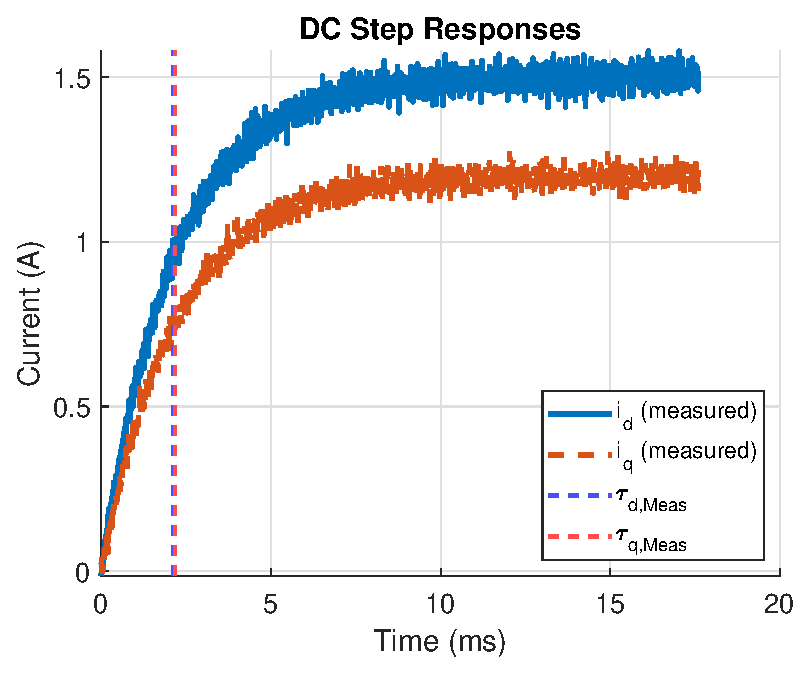
\includegraphics[width=\textwidth]{./InductanceMeas}
	\caption{DC-Step Test for Motor Inductance Measurements}
	\label{fig:InductanceMeas}
\end{figure}


With the previously identified per-phase resistance \(R_s=1.25~\Omega\), the motor inductances are then computed by the following equations:
\begin{equation}
\label{eq:Ld-from-tau-osc}
L_d \;=\; R_s\,\tau_d, 
\qquad
L_q \;=\; R_s\,\tau_q,
\end{equation}

Following the procedure above, \(\tau_d\) equals 2.1227~\text{ms}  and \(\tau_q\) equals 2.1716~\text{ms} were read from the oscilloscope, and the inductances were computed via \eqref{eq:Ld-from-tau-osc} with \(R_s=1.25~\Omega\), yielding
\[
L_d=2.67~\text{mH},\qquad L_q=2.75~\text{mH}.
\]
These are the inductance values used in the electrical model and subsequent controller design.

MEASUREMENT SETUP SHOT FROM THE LAB HAS TO BE INCLUDED HERE.

\subsection{Motor Flux Linkage Measurement}
\label{subsec:lambda-emf-ll}

The motor is driven as a generator by a prime mover at \(1000~\mathrm{rpm}\) with open stator terminals. Using a differential probe, the line–to–line no-load back-EMF is recorded on the oscilloscope as shown in Figure~\ref{fig:FluxLinkage} and its fundamental RMS value \(E_{\mathrm{LL,rms}}\) is extracted (single-tone FFT or narrowband filter at the electrical frequency). With pole–pair count \(p=4\), the speeds are
\[
\omega_m = 2\pi\frac{1000}{60}\ \text{rad/s},\qquad
\omega_e = p\,\omega_m,
\]
and the flux linkage is computed directly from the scope measurement by
\[
\lambda_f \;=\; \frac{\sqrt{2}}{\sqrt{3}}\;\frac{E_{\mathrm{LL,rms}}}{\omega_e}.
\]

Applying the above with the oscilloscope-measured \(E_{\mathrm{LL,rms}}\) at \(1000~\mathrm{rpm}\) gives
\[
\boxed{\lambda_f = 0.1227~\text{Wb}}.
\]

\begin{figure}[h]
	\centering
	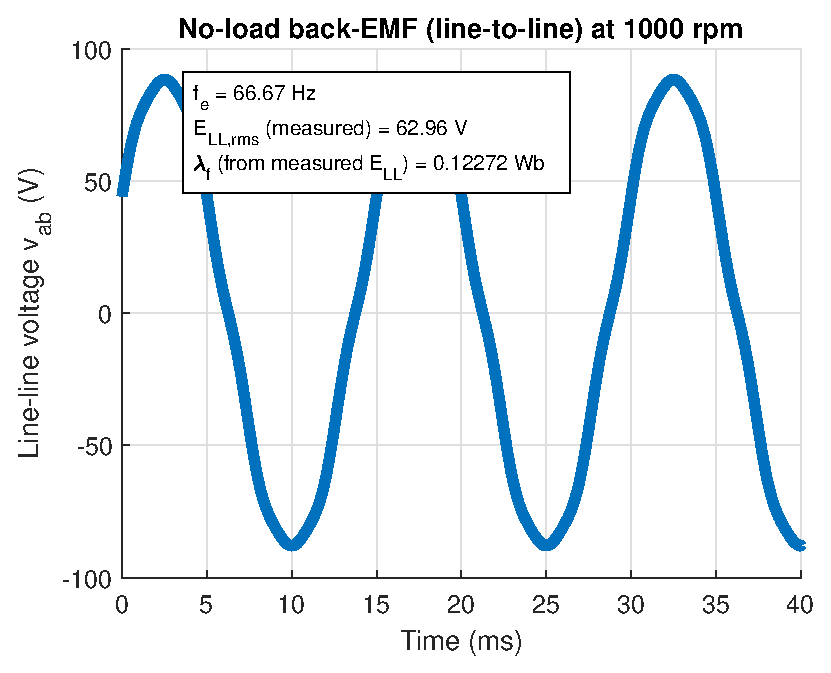
\includegraphics[width=\textwidth]{./FluxLinkageMeas}
	\caption{No-Load back-EMF Test at 1000 RPM}
	\label{fig:FluxLinkage}
\end{figure}


\subsection{Viscous Friction Measurement}
\label{subsec:viscous-friction}

The motor is driven at a sequence of constant mechanical speeds covering the operating range (e.g., from low rpm up to the rated region). At each target speed the drive is held until the signals stabilize—i.e., the speed derivative is negligible and the torque/current readings have settled—so that transients are removed. The steady values \((\omega_m,\,T_e)\) are then logged. Repeating this for all speed points produces a set of steady-state pairs suitable for identification.

A smooth curve of torque versus speed is drawn by interpolating the measured points to aid visualization. The friction parameters are obtained by fitting the standard affine model
\[
T_e(\omega_m)=B\,\omega_m+T_c,
\]
where the slope \(B\) is the viscous friction coefficient \([\mathrm{N\,m\,s/rad}]\) and the \emph{intercept} \(T_c\) is the constant (Coulomb) friction torque \([\mathrm{N\,m}]\). The line fit (ordinary least squares) is performed on the measured \((\omega_m,\,T_e)\) data as shown in Figure~\ref{fig:ViscousFriction}.

\begin{figure}[H]
	\centering
	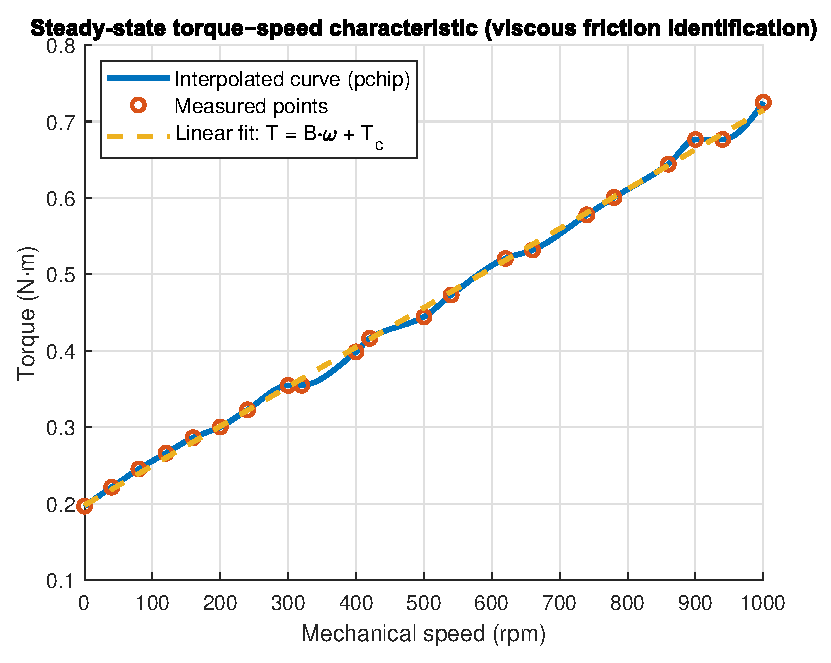
\includegraphics[width=\textwidth]{./ViscousFriction}
	\caption{Steady-State Torque-Speed Characteristic Test for Viscous Friction Identification}
	\label{fig:ViscousFriction}
\end{figure}

\subsection{Motor Inertia Measurement}
\label{subsec:inertia-coastdown}

The rotor inertia \(J\) is identified from a \emph{free deceleration} test. The motor is accelerated to a target speed and then commanded to zero electromagnetic torque (e.g., \(i_q\!\to\!0\) or inverter disabled). The mechanical speed \(\omega_m(t)\) is logged until near standstill. Under the viscous–Coulomb friction model used in this chapter,
\[
J\,\dot{\omega}_m \;=\; -\,B\,\omega_m \;-\; T_c,
\]
so a linear fit of \(\dot{\omega}_m\) versus \(\omega_m\) yields \(\dot{\omega}_m = a\,\omega_m + b\) with \(a=-B/J\) and \(b=-T_c/J\). 

Applying the above to the recorded coast–down data and using \(B=0.004775~\mathrm{N\,m\,s/rad}\) and \(T_c=0.2~\mathrm{N\,m}\), the identified rotor inertia is
\[
\boxed{J = 0.00636~\mathrm{kg\,m^2}}.
\]

\section{Inverter Non-Linearities Average Model for a Two-Level VSI}
\label{sec:vsi-nonlinear-model}

\subsection{Analytical Modeling}
In a PWM two-level voltage-source inverter (VSI) the actual pole voltages differ from the ideal SVM targets because of dead time, finite turn-on/off delays, and device on-state drops in the transistor and anti-parallel diode. The resulting mismatch introduces low-frequency distortion in the phase voltages, which propagates to current ripple, harmonic torque, and degraded tracking effects that are well documented in the literature. 

Consider one switching period \(T_s\). Let \(T_u^\ast,T_v^\ast,T_w^\ast\) be the ideal upper-device on-times produced by SVM. Practical gating inserts a dead interval so that each leg conducts slightly less (or slightly more) than scheduled depending on the current polarity. Defining \(\operatorname{sgn}(i_{ph})\!:=\!+1\) as shown in (\ref{eq:phasedir}) if the phase current flows into the machine and \(-1\) otherwise (sign convention as in Figure \ref{fig:InverterNonlinearities}), the average phase-to-neutral voltage including dead time \(t_{\mathrm{dead}}\), commutation skews \(t_{\mathrm{ON}},t_{\mathrm{OFF}}\), and device drops is given, per phase \(u\), by the standard form (\ref{eq:vun}), and (\ref{eq:vun_star}):

\begin{figure}[h]
	\centering
	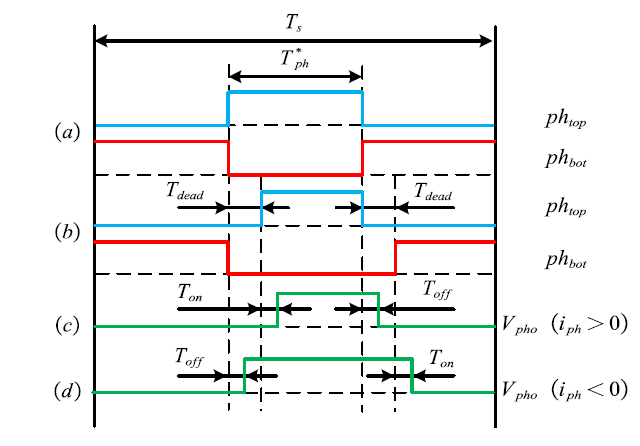
\includegraphics[width=\textwidth]{./InverterNonlinearities}
	\caption{Ideal versus non-ideal switching and the resulting phase voltage: (a) ideal gating waveforms; (b) gating with inserted dead time; (c) actual phase voltage for \(i_{ph}>0\); (d) actual phase voltage for \(i_{ph}<0\).}
	\label{fig:InverterNonlinearities}
\end{figure}


\begin{equation}
\label{eq:phasedir}
\operatorname{sgn}(i_{ph}) =
\begin{cases}
  1,  & i_{ph} > 0,\\[2pt]
 -1,  & i_{ph} < 0.
\end{cases}
\end{equation}

\begin{equation}
\label{eq:vun}
v_{un}=\frac{V_{\!dc}-V_{\!CE}+V_D}{3T_s}\,\bigl(2T_u-T_v-T_w\bigr)
-\frac{V_{CE0}+V_{D0}}{6}\bigl(2\,\operatorname{sgn}i_u-\operatorname{sgn}i_v-\operatorname{sgn}i_w\bigr)
-\frac{R_{CE}+R_D}{2}\,i_u,
\end{equation}
with the ideal counterpart
\begin{equation}
\label{eq:vun_star}
v_{un}^\ast=\frac{V_{\!dc}-V_{\!CE}+V_D}{3T_s}\,\bigl(2T_u^\ast-T_v^\ast-T_w^\ast\bigr).
\end{equation}
Here the transistor and diode drops are captured by the usual current\-dependent linearizations
\begin{equation}
\label{eq:lin-drops}
V_{\!CE}=V_{CE0}+R_{CE}\,\lvert i_{\!ph}\rvert,\qquad
V_D=V_{D0}+R_D\,\lvert i_{\!ph}\rvert,
\end{equation}
and the \emph{dead-time kernel}
\begin{equation}
\label{eq:Lambda}
\Lambda=\frac{(V_{\!dc}-V_{\!CE}+V_D)\,(t_{\mathrm{dead}}+t_{\mathrm{ON}}-t_{\mathrm{OFF}})}{3T_s}+\frac{V_{CE0}+V_{D0}}{6}
\end{equation}
collects the polarity-dependent bias. Equations \eqref{eq:vun}–\eqref{eq:Lambda} summarize the combined effect of dead time, timing skews, and device drops on the average phase voltage.

Stacking the three phases, the error \(\boldsymbol{v}_{\!err}=\boldsymbol{v}^\ast-\boldsymbol{v}\) admits a compact expression:
\begin{equation}
\label{eq:verr-abc}
\begin{bmatrix} v_{un}^{err}\\ v_{vn}^{err}\\ v_{wn}^{err}\end{bmatrix}
=\Lambda
\begin{bmatrix} 2&-1&-1\\ -1&2&-1\\ -1&-1&2\end{bmatrix}
\begin{bmatrix}\operatorname{sgn}i_u\\ \operatorname{sgn}i_v\\ \operatorname{sgn}i_w\end{bmatrix}
+\frac{R_{CE}+R_D}{2}\begin{bmatrix} i_u\\ i_v\\ i_w\end{bmatrix}.
\end{equation}
This makes two ingredients explicit: (i) a polarity kernel driven by current signs that flips as the phase currents cross zero, and (ii) a small resistive drop proportional to phase current.

Using the Clarke–Park transformations, the theoretical distortion voltages appearing in the synchronous model are
\begin{equation}
\label{eq:vdqth}
\begin{bmatrix} v_d^{th}\\ v_q^{th}\end{bmatrix}
= \;3\,K_{3s\!\to r}\,\Lambda
\begin{bmatrix}\operatorname{sgn}i_u\\ \operatorname{sgn}i_v\\ \operatorname{sgn}i_w\end{bmatrix}
+K_{3s\!\to r}\,\frac{R_{CE}+R_D}{2}\begin{bmatrix} i_u\\ i_v\\ i_w\end{bmatrix},
\end{equation}
where \(K_{3s\!\to r}\) is the standard \(3\! \to\! 2\) Park matrix evaluated at electrical angle \(\theta_e\),
\begin{equation}
\label{eq:K32}
K_{3s\!\to r}=\frac{2}{3}
\begin{pmatrix}
\cos\theta_e & \cos(\theta_e\!-\!2\pi/3) & \cos(\theta_e\!+\!2\pi/3)\\[2pt]
-\sin\theta_e & -\sin(\theta_e\!-\!2\pi/3) & -\sin(\theta_e\!+\!2\pi/3)
\end{pmatrix}\!.
\end{equation}
In this form the non\-idealities enter the \(dq\) electrical equations as an additive bias to the commanded voltages. The cited analysis further notes that bus voltage and dead time dominate the distortion magnitude; the impact weakens as operating speed rises, and the dominant ripple in \(dq\) appears around \(6\omega_e\) (six times the electrical frequency), consistent with three\-phase symmetry. 

With \(\boldsymbol{v}_{dq}^{th}\) known from \eqref{eq:vdqth}, the synchronous PMSM model reads
\begin{equation}
\label{eq:pmsm-with-dist}
\begin{bmatrix} v_d\\ v_q\end{bmatrix}
=\begin{bmatrix} R & -\omega_e L_q\\ \omega_e L_d & R\end{bmatrix}
\begin{bmatrix} i_d\\ i_q\end{bmatrix}
+\begin{bmatrix} 0\\ \omega_e\lambda_f\end{bmatrix}
+\begin{bmatrix} v_d^{th}\\ v_q^{th}\end{bmatrix},
\end{equation}
so that any controller (PI, MPC, or observer\-based) can treat \([v_d^{th}\ v_q^{th}]^\top\) as a known feedforward bias (``theoretical'' part) and reserve an estimator for the small residual coming from parameter spread or temperature.


\subsection{PI Controller Simulation Modeling Under Inverter-Nonlinearities Effects}
This section validates the complete drive model and controllers through a focused suite of studies: (i) steady-state operation to verify ripple, losses, and harmonic content; (ii) low-speed operation to probe back-EMF limits and non-idealities; (iii)  dynamic performance under speed/current steps; (iv) parameter variation to gauge robustness against model mismatch; and (v) load variation to assess torque disturbance rejection.
\subsubsection{Steady State Operation}
With dead time and device drops enabled, the PI drive at 1000 rpm exhibits high harmonic content that a moderate-bandwidth controller (\(\approx\)20~Hz) cannot suppress. At \emph{low load} (10\% rated torque, \(0.3~\mathrm{N\,m}\)) the phase-current THD reaches 16.4\% (see Fig.~\ref{fig:PINL_1000rpm_low}); at \emph{medium load} (50\% rated torque, \(1.75~\mathrm{N\,m}\)) it falls to 4.3\% (see Fig.~\ref{fig:PINL_1000rpm_med}). The pattern is consistent with PWM non-idealities injecting polarity-dependent voltage biases that map, via three-phase symmetry, into prominent \(5^\text{th}\) and \(7^\text{th}\) harmonics; because these behave as additive voltage sources rather than simple plant shifts, a PI loop with limited crossover cannot reject them effectively, yielding elevated THD even though average torque and speed regulation remain correct.

\begin{figure}[H]
  \centering
  % --- (a) Low load under non-ideal inverter ---
  \begin{subfigure}{0.485\textwidth}
    \centering
    % Replace with your exported plot/image
    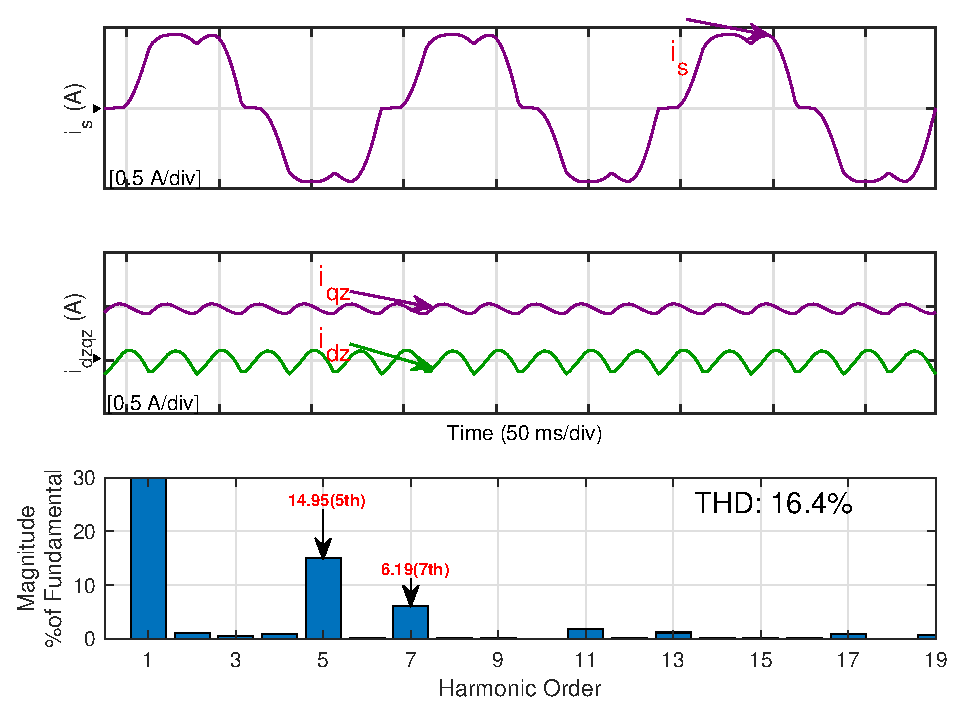
\includegraphics[width=\linewidth]{./PIMidSpeedLowLoadSteadyState}
    \caption{Low load: \(T=0.3~\mathrm{N\,m}\). \\THD \(=16.4\%\).}
    \label{fig:PINL_1000rpm_low}
  \end{subfigure}\hfill
  % --- (b) Medium load under non-ideal inverter ---
  \begin{subfigure}{0.485\textwidth}
    \centering
    % Replace with your exported plot/image
    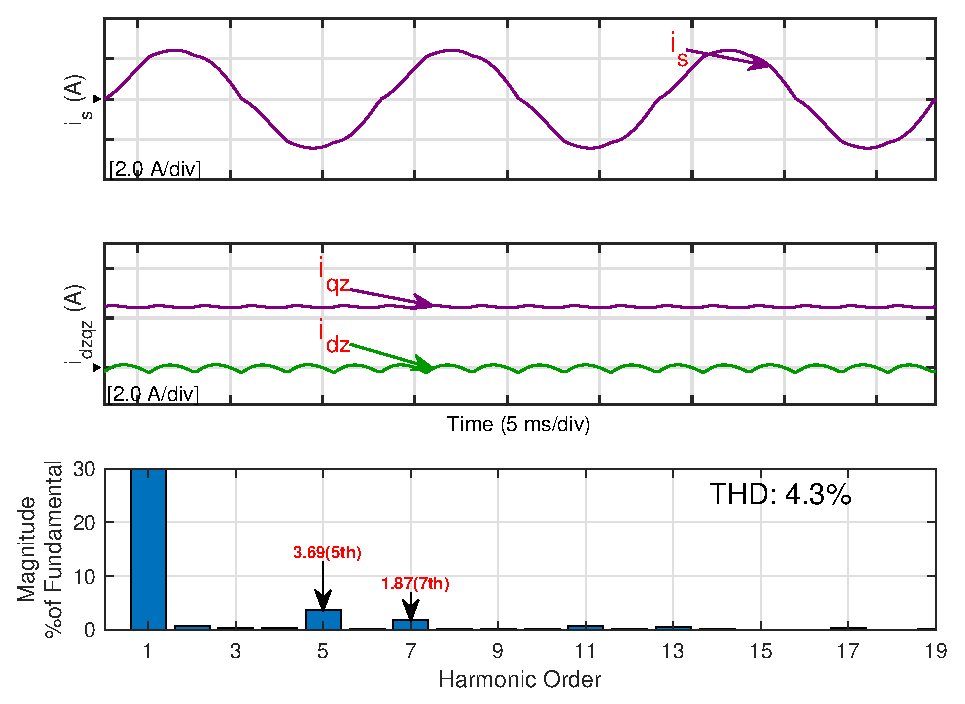
\includegraphics[width=\linewidth]{./PIMidSpeedMidLoadSteadyState}
    \caption{Medium load: \(T=1.75~\mathrm{N\,m}\).\\ THD \(=4.3\%\).}
    \label{fig:PINL_1000rpm_med}
  \end{subfigure}

  \caption{PI steady-state at 50\% rated speed (1000 rpm) with inverter non-linearities enabled (dead time, device drops). The figure reports  phase currents, \(d\)- and \(q\)-axis currents, and the THD.}
  \label{fig:PINL_1000rpm}
\end{figure}

\subsubsection{Low Speed Operation}
With dead time and device drops enabled, the PI drive at 200 rpm (10\% rated) shows pronounced distortion: at low load (10\% rated torque, \(0.3~\mathrm{N\,m}\)) the phase-current THD reaches 23.2\% (Fig.~\ref{fig:PINL_200rpm_low}), while at high load (100\% rated torque, \(3.5~\mathrm{N\,m}\)) it falls to 6.9\% (Fig.~\ref{fig:PINL_200rpm_high}). The pattern reflects polarity-dependent voltage biases that project into strong odd harmonics (notably \(5^\text{th}\)/\(7^\text{th}\)), which a PI loop with \(\approx\)20~Hz crossover cannot effectively reject. At 100 rpm (5\% rated), the same non-idealities consume much of the voltage headroom and the loop fails to settle—see Fig.~\ref{fig:PINL_100rpm_unstable}—indicating insufficient robustness of the present PI design in this extreme low-speed, non-ideal regime.

% Requires in preamble:
% \usepackage{graphicx}
% \usepackage{subcaption}

% ---------- PI @ 10% rated (200 rpm) under inverter non-linearities ----------
\begin{figure}[H]
  \centering
  % Low load (10% rated torque)
  \begin{subfigure}{0.485\textwidth}
    \centering
    % Replace with your exported plot/image
    
\includegraphics[width=\linewidth]{./PISteadyStateLowLoad200Rpm}
    \caption{Low load: \(T=0.3~\mathrm{N\,m}\). THD \(=23.2\%\).}
    \label{fig:PINL_200rpm_low}
  \end{subfigure}\hfill
  % High/rated load (100% rated torque)
  \begin{subfigure}{0.485\textwidth}
    \centering
    % Replace with your exported plot/image
    
\includegraphics[width=\linewidth]{./PISteadyStateHighLoad200Rpm}
    \caption{Rated load: \(T=3.5~\mathrm{N\,m}\). THD \(=6.9\%\).}
    \label{fig:PINL_200rpm_high}
  \end{subfigure}

  \caption{PI controller at 200 rpm (10\% rated) with inverter non-linearities enabled (dead time, device drops). Each panel shows The figure reports  phase currents, \(d\)- and \(q\)-axis currents, and the THD. Prominent odd harmonics (notably 5th/7th) elevate THD at low load; the higher fundamental at rated load reduces the relative distortion.}
  \label{fig:PINL_200rpm}
\end{figure}

% ---------- PI @ 5% rated (100 rpm) under inverter non-linearities: unstable case ----------
\begin{figure}[H]
  \centering
  % Replace with your exported plot/image
  
\includegraphics[width=0.6\linewidth]{./PISteadyStateLowLoad100Rpm}
  \caption{PI controller at 100 rpm (5\% rated) with inverter non-linearities enabled. The combination of dead time/device drops and limited loop bandwidth leads to failure to settle (unstable/oscillatory response). The figure reports  phase currents, \(d\)- and \(q\)-axis currents, and the THD.}
  \label{fig:PINL_100rpm_unstable}
\end{figure}

\subsubsection{Dynamic Performance}
With dead time and device drops enabled, speed steps within the 5–50\% band reveal a low-speed limitation: when the request includes 5\% (100~rpm), the PI loop fails to settle at both low load and rated load. For commands \(\mathbf{\ge}10\%\) of rated (200–1000~rpm), the same controller tracks cleanly with well-damped transients and negligible steady-state error. These behaviors are consolidated in the two summary plots: Fig.~\ref{fig:PINL_Dyn_low} (low load, multiple speed transitions) and Fig.~\ref{fig:PINL_Dyn_rated} (rated load, multiple speed transitions).

\begin{figure}[H]
  \centering
  % --- (a) Low load ---
  \begin{subfigure}{0.485\textwidth}
    \centering
    % Replace with your exported plot/image stacking multiple speed transitions
    
\includegraphics[width=\linewidth]{./DynamicResponsePILowLoad}
    \caption{Low load (\(T=0.3~\mathrm{N\,m}\)). Includes 5–50\% speed transitions; fails to settle at 5\% (100 rpm), tracks cleanly for \(\ge\)10\%.}
    \label{fig:PINL_Dyn_low}
  \end{subfigure}\hfill
  % --- (b) Rated load ---
  \begin{subfigure}{0.485\textwidth}
    \centering
    % Replace with your exported plot/image stacking multiple speed transitions
    
\includegraphics[width=\linewidth]{./DynamicResponsePIHighLoad}
    \caption{Rated load (\(T=3.5~\mathrm{N\,m}\)). Same behavior: unstable at 5\%, well-damped for \(\ge\)10\%.}
    \label{fig:PINL_Dyn_rated}
  \end{subfigure}

  \caption{PI dynamic performance under inverter non-linearities (dead time, device drops) with multiple speed transitions in the 5–50\% band. Each subfigure shows command vs.\ speed, \(i_q\), and phase currents. The controller fails to settle at 5\% (100 rpm) but tracks cleanly for \(\ge\)10\% of rated speed across both load conditions.}
  \label{fig:PINL_Dyn}
\end{figure}

\subsubsection{Parameter Variation}
To probe worst-case robustness, the PI controller was evaluated at 10\% rated speed (200~rpm) with inverter non-idealities (dead time, device drops) while the motor model used for tuning was biased by \(R_s{+}25\%\) and \(L_{d,q}{-}25\%\). This perturbation shortens the electrical time constant (\(\tau=L/R \rightarrow 0.60\,\tau\)), shifts the plant pole, and detunes the PI crossover/cutoff relative to the true plant. As illustrated in Fig.~\ref{fig:PINL_ParamVariation}, the phase-current THD increases from 23.2\% (nominal parameters) to 24.2\% under the bias—a modest but measurable degradation consistent with reduced disturbance-rejection margin when the PI bandwidth drifts in the presence of additive inverter distortion.
\begin{figure}[H]
  \centering
  % Replace with your exported composite plot (e.g., speed, dq-currents, phase currents, THD bars)
  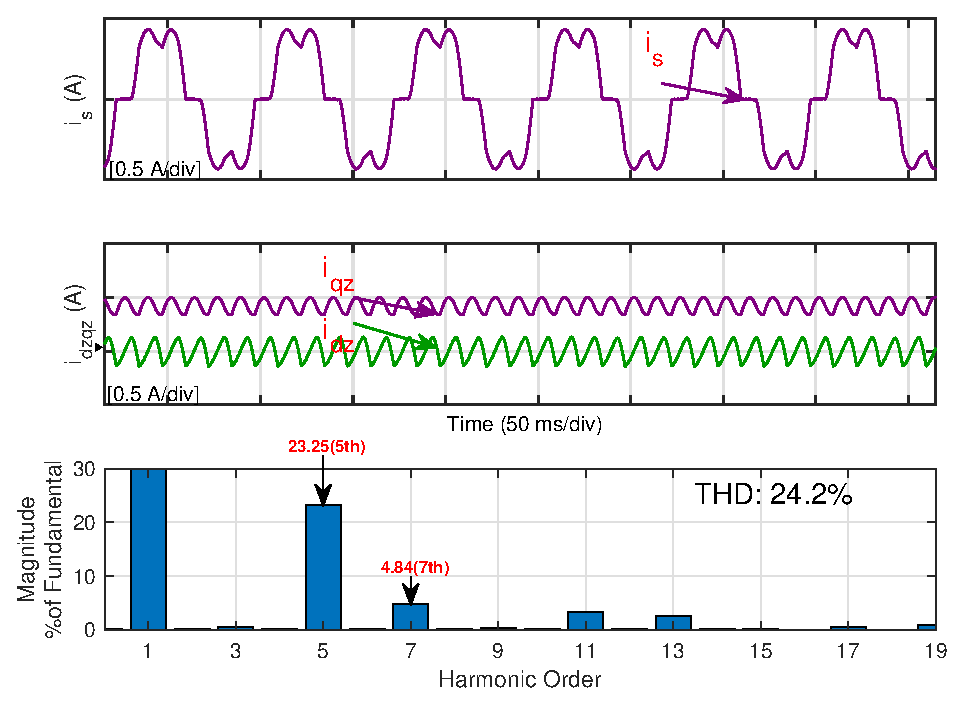
\includegraphics[width=0.8\linewidth]{./PIParameterVariation}
  \caption{PI controller under parameter variation with inverter non-linearities at 200 rpm (10\% rated).}
  \label{fig:PINL_ParamVariation}
\end{figure}

\subsubsection{Load Variation}	
With dead time and device drops enabled, the motor was held at 1000 rpm while the load torque was stepped from 10\% to 100\% of rated in 20\% increments, each plateau maintained to steady state. As shown in Fig.~\ref{fig:PINL_LoadVariation}, the PI loop preserves the commanded speed without appreciable droop; the \(q\)-axis current \(i_q\) rises in clean, proportional steps to furnish the added torque, and the phase currents—though exhibiting extra ripple from non-idealities—remain bounded and well behaved. Transients are short and well damped across all steps, evidencing robust disturbance rejection despite the inverter’s harmonic bias.
% Requires in preamble:
% \usepackage{graphicx}

\begin{figure}[H]
  \centering
  % Replace with your exported composite plot:
  % (left) speed response, (middle) q-axis current, (right) phase currents
  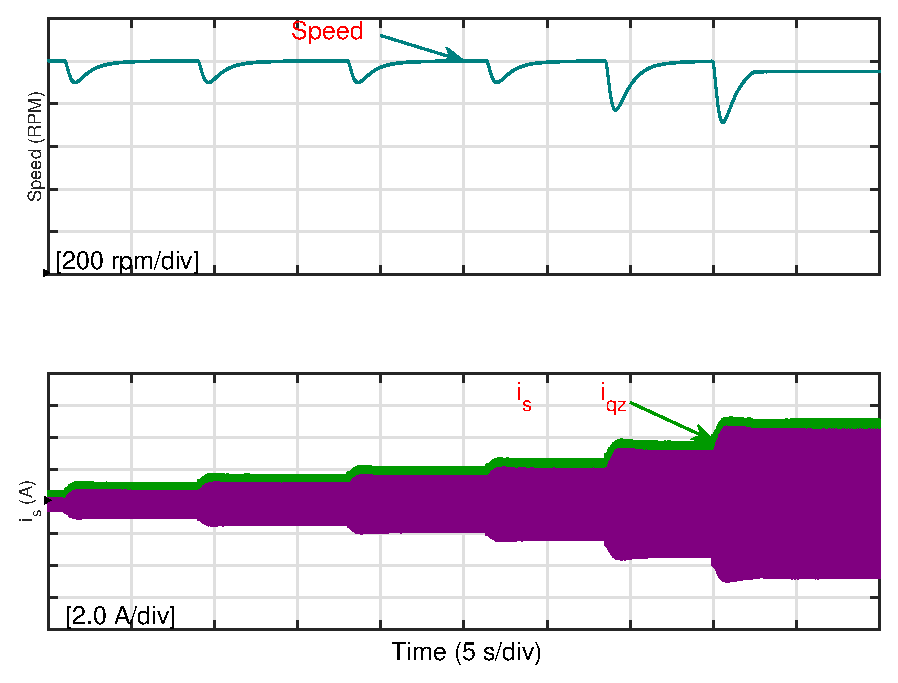
\includegraphics[width=0.6\linewidth]{./PILoadVariation}
  \caption{PI controller under load variation at 50\% rated speed (1000 rpm) with inverter non-linearities
  (dead time, device drops). The composite plot shows motor speed, \(i_q\), and phase currents during torque steps
  from 10\% to 100\% of rated in 20\% increments.}
  \label{fig:PINL_LoadVariation}
\end{figure}

\subsection{Finite Control Set Model Predictive Simulation Modeling Under Inverter-Nonlinearities Effects}
\subsubsection{Steady State Operation}
With dead time and device drops enabled, the FCS–MPC at 1000 rpm and 50\% rated load (\(1.75~\mathrm{N\,m}\)) yields a phase–current THD of 17\% (see Fig.~\ref{fig:FCSNL_1000rpm_med}). The elevated distortion is consistent with single–vector actuation interacting with polarity–dependent voltage biases to project strong odd harmonics—especially \(5^\text{th}\) and \(7^\text{th}\). At this operating point the THD is slightly higher than the PI baseline reported at the same speed (\(\approx\)16.4\%; see Fig.~\ref{fig:PINL_1000rpm_low}).

\begin{figure}[H]
  \centering
  % Replace with your exported plot/image
  
\includegraphics[width=0.6\linewidth]{FCSMidSpeedMidLoadSteadyState}
  \caption{FCS–MPC steady state at 50\% rated speed (1000 rpm) and 50\% rated load (\(1.75~\mathrm{N\,m}\)) with inverter non-linearities (dead time, device drops). The plot shows phase currents, \(d\)- and \(q\)-axis currents, and THD.}
  \label{fig:FCSNL_1000rpm_med}
\end{figure}

\subsubsection{Low Speed Operation}
With dead time and device drops enabled, the FCS–MPC struggles at the most challenging operating point: in sensorless mode at 5\% rated speed (100~rpm) and low load, the controller cannot stabilize because the weak back-EMF and single-vector actuation make the effective voltage quantization too coarse for reliable angle/torque regulation. From 10\% rated (200~rpm) upward the loop settles; at low load the harmonic content remains high—THD 34\%, as shown in Fig.~\ref{fig:FCSNL_200rpm_low}—whereas at high load the larger commanded voltage reduces the vector mismatch and THD drops to 5.6\%, see Fig.~\ref{fig:FCSNL_200rpm_high}. Compared to PI at the same conditions (23\% at low load, 6.9\% at high load), FCS is inferior at light load but shows an advantage at high torque.
% Requires in preamble:
% \usepackage{graphicx}
% \usepackage{subcaption}

\begin{figure}[H]
  \centering
  % --- (a) Low load @ 10% speed (200 rpm) ---
  \begin{subfigure}{0.485\textwidth}
    \centering
    % Replace with your exported plot/image
    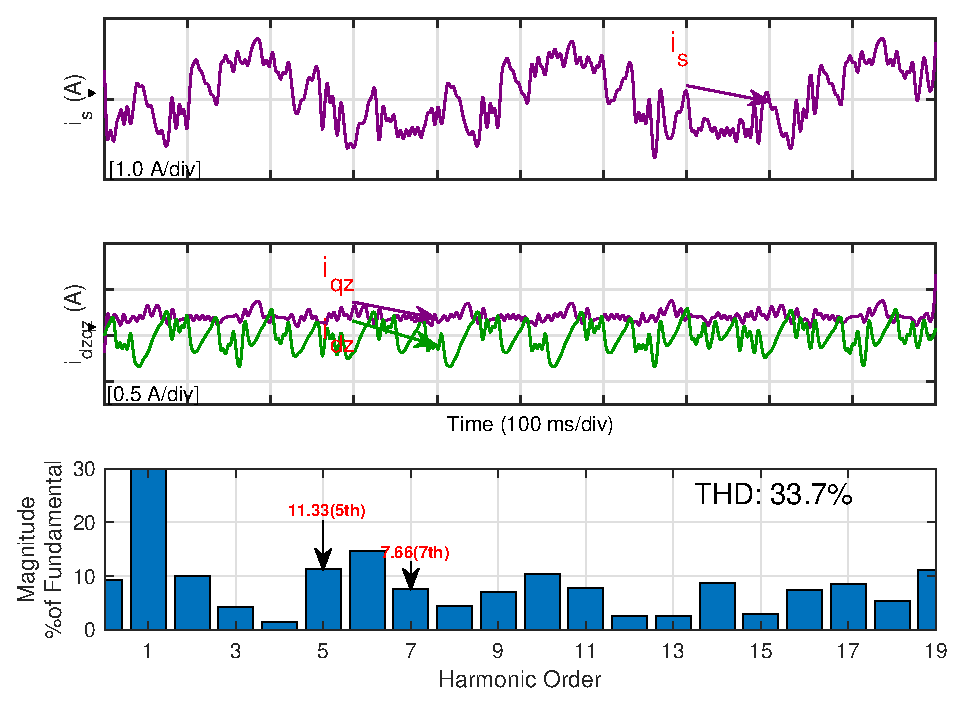
\includegraphics[width=\linewidth]{FCSSteadyStateLowLoad200Rpm}
    \caption{Low load: \(T=0.3~\mathrm{N\,m}\). THD \(=34\%\).}
    \label{fig:FCSNL_200rpm_low}
  \end{subfigure}\hfill
  % --- (b) High/rated load @ 10% speed (200 rpm) ---
  \begin{subfigure}{0.485\textwidth}
    \centering
    % Replace with your exported plot/image
    
\includegraphics[width=\linewidth]{FCSSteadyStateHighLoad200Rpm}
    \caption{Rated load: \(T=3.5~\mathrm{N\,m}\). THD \(=5.6\%\).}
    \label{fig:FCSNL_200rpm_high}
  \end{subfigure}

  \caption{FCS–MPC at 10\% rated speed (200 rpm) with inverter non-linearities (dead time, device drops). 
  Each panel shows phase currents, \(i_{dq}\), and THD.}
  \label{fig:FCSNL_200rpm}
\end{figure}

\subsubsection{Dynamic Performance}
With dead time and device drops enabled, the FCS–MPC was commanded over 5–50\% rated (100–1000~rpm) at \emph{low load} (\(0.3~\mathrm{N\,m}\)). As shown in Fig.~\ref{fig:FCSNL_Dyn_low}, tracking at higher set-points is acceptable, but the step-down to 10\% (200~rpm) loses stability: weak back-EMF and additive voltage bias degrade the sensorless angle SNR, bias one-step predictions, and—under single-vector actuation—lead to suboptimal vector choices and coarse staircase voltages; the loop oscillates and fails to settle, evidencing degraded dynamic robustness in this regime.
% Requires in preamble:
% \usepackage{graphicx}

\begin{figure}[H]
  \centering
  % Replace with your exported plot/image for the low-load dynamic test
  
\includegraphics[width=0.6\linewidth]{./FCSDynamicResponseLowLoad}
  \caption{FCS–MPC dynamic performance under inverter non-linearities at low load (\(T=0.3~\mathrm{N\,m}\)).
  The figure aggregates multiple speed transitions within the 5–50\% rated band (100–1000 rpm), showing command vs.\ speed,
  \(d\)- and \(q\)-axis currents, and phase currents.}
  \label{fig:FCSNL_Dyn_low}
\end{figure}

\subsubsection{Parameter Variation}
At 10\% rated speed (200~rpm) with dead time and device drops enabled, the FCS–MPC was run using a deliberately biased prediction model (\(R_s{+}25\%\), \(L_{d,q}{-}25\%\)) while the plant remained unchanged. As illustrated in Fig.~\ref{fig:FCSNL_ParamVariation}, under the low-load case (\(T\!\approx\!0.3~\mathrm{N\,m}\)) the phase-current THD increases from 34\% (nominal model) to 40\%. This is characteristic of FCS: one-step predictions pick a single vector each sample, so \(R\!-\!L\) errors misrank candidates and, in the presence of polarity-dependent inverter biases, exacerbate the staircase voltage, amplifying harmonics and torque ripple.
% Requires in preamble:
% \usepackage{graphicx}

\begin{figure}[H]
  \centering
  % Replace with your exported composite plot (e.g., speed, dq currents, phase currents, THD bars)
  
\includegraphics[width=0.6\linewidth]{FCSParameterVariation}
  \caption{FCS–MPC with inverter non-linearities (dead time, device drops) under parameter variation at 10\% rated speed (200 rpm, low load \(T\!\approx\!0.3~\mathrm{N\,m}\)).
  The prediction model is biased with \(R_s{+}25\%\) and \(L_{d,q}{-}25\%\) while the plant is unchanged. The composite plot shows \(d\)- and \(q\)-axis currents, phase currents, and THD.}
  \label{fig:FCSNL_ParamVariation}
\end{figure}

\subsubsection{Load Variation}
With dead time and device drops enabled, the motor was held at 1000 rpm while the load torque stepped from 10\% to 100\% of rated in 20\% increments. As shown in Fig.~\ref{fig:FCSNL_LoadVariation}, the FCS–MPC maintains the commanded speed without failures or steady-state deviation—\(i_q\) rises in proportional steps and the average torque matches the request—yet the phase currents exhibit pronounced ripple and the electromagnetic torque shows a high ripple floor. This follows from FCS’s single-vector actuation, whose staircase phase voltage, compounded by polarity-dependent inverter biases, injects strong low-order harmonics despite robust regulation during the load sweep.
% Requires in preamble:
% \usepackage{graphicx}

\begin{figure}[H]
  \centering
  % Replace with your exported composite plot (speed, i_q, phase currents, torque ripple if available)
  
\includegraphics[width=0.6\linewidth]{FCSLoadVariation}
  \caption{FCS–MPC under load variation at 50\% rated speed (1000 rpm) with inverter non-linearities
  (dead time, device drops). The composite plot shows motorspeed, \(i_q\), and phase currents during torque steps
  from 10\% to 100\% of rated in 20\% increments.}
  \label{fig:FCSNL_LoadVariation}
\end{figure}

\subsection{Modulated Model Predictive Controller Simulation Modeling Under Inverter-Nonlinearities Effects}
\subsubsection{Steady State Operation}
With dead time and device drops enabled at 1000 rpm, the M2PC sustains tight regulation and markedly lower distortion than PI or FCS across loads. At \emph{low load} (10\% rated torque, \(0.3~\mathrm{N\,m}\)) the phase-current THD is 8\% (vs.\ \(\sim\)16\% for PI), see Fig.~\ref{fig:M2PCNL_1000rpm_low}; at medium load (50\% rated torque, \(1.75~\mathrm{N\,m}\)) it falls to 2\% (vs.\ \(\sim\)4\% for PI and \(\sim\)17\% for FCS), see Fig.~\ref{fig:M2PCNL_1000rpm_med}. The advantage stems from optimizing a continuous average voltage each sample and realizing it via fixed-frequency SVM, which concentrates spectral energy at the carrier and treats non-idealities as additive biases that can be explicitly compensated—thereby suppressing the staircase ripple that penalizes FCS and outperforming the moderate-bandwidth PI loop at the same operating point.

\begin{figure}[H]
  \centering
  % --- (a) Low load (10% rated torque) ---
  \begin{subfigure}{0.485\textwidth}
    \centering
    % Replace with your exported plot/image
    
\includegraphics[width=\linewidth]{MPCMidSpeedLowLoadSteadyState}
    \caption{Low load: \(T=0.3~\mathrm{N\,m}\). \\THD \(=8\%\).}
    \label{fig:M2PCNL_1000rpm_low}
  \end{subfigure}\hfill
  % --- (b) Medium load (50% rated torque) ---
  \begin{subfigure}{0.485\textwidth}
    \centering
    % Replace with your exported plot/image
    
\includegraphics[width=\linewidth]{MPCMidSpeedMidLoadSteadyState}
    \caption{Medium load: \(T=1.75~\mathrm{N\,m}\).\\ THD \(=2\%\).}
    \label{fig:M2PCNL_1000rpm_med}
  \end{subfigure}

  \caption{M2PC steady state at 50\% rated speed (1000 rpm) with inverter non-linearities (dead time, device drops). Each panel shows \(i_{dq}\), phase currents, and THD at both load levels.}
  \label{fig:M2PCNL_1000rpm}
\end{figure}

\newpage
\subsubsection{Low Speed Operation}
With dead time and device drops enabled, the M2PC remains robust in sensorless operation at very low speeds. At 5\% rated (100~rpm), the phase-current THD is 6.9\% at low load (\(0.3~\mathrm{N\,m}\), see Fig.~\ref{fig:M2PCNL_100rpm_low}) and 1.1\% at rated load (\(3.5~\mathrm{N\,m}\), see Fig.~\ref{fig:M2PCNL_100rpm_high}); at this speed both PI and FCS are unstable. At 10\% rated (200~rpm), MPC yields 6.6\% THD at low load (\(0.5~\mathrm{N\,m}\), see Fig.~\ref{fig:M2PCNL_200rpm_low}) and 1.1\% at rated load (\(3.5~\mathrm{N\,m}\), see Fig.~\ref{fig:M2PCNL_200rpm_high}), compared to \(\sim\)34\%/5.6\% for FCS and \(\sim\)23\%/6.9\% for PI.
% Requires in preamble:
% \usepackage{graphicx}
% \usepackage{subcaption}

\begin{figure}[H]
  \centering

  % --- (a) 5% rated (100 rpm), low load ---
  \begin{subfigure}{0.485\textwidth}
    \centering
    
\includegraphics[width=\linewidth]{./MPCSteadyStateLowLoad100Rpm}
    \caption{5\% speed (100 rpm), low load \(T=0.3~\mathrm{N\,m}\); THD \(=6.9\%\).}
    \label{fig:M2PCNL_100rpm_low}
  \end{subfigure}\hfill
  % --- (b) 5% rated (100 rpm), rated load ---
  \begin{subfigure}{0.485\textwidth}
    \centering
    
\includegraphics[width=\linewidth]{./MPCSteadyStateHighLoad100Rpm}
    \caption{5\% speed (100 rpm), rated load \(T=3.5~\mathrm{N\,m}\); THD \(=1.1\%\).}
    \label{fig:M2PCNL_100rpm_high}
  \end{subfigure}

  \vspace{0.6em}

  % --- (c) 10% rated (200 rpm), low load ---
  \begin{subfigure}{0.485\textwidth}
    \centering
    
\includegraphics[width=\linewidth]{./MPCSteadyStateLowLoad200Rpm}
    \caption{10\% speed (200 rpm), low load \(T=0.5~\mathrm{N\,m}\); THD \(=6.6\%\).}
    \label{fig:M2PCNL_200rpm_low}
  \end{subfigure}\hfill
  % --- (d) 10% rated (200 rpm), rated load ---
  \begin{subfigure}{0.485\textwidth}
    \centering
    
\includegraphics[width=\linewidth]{./MPCSteadyStateHighLoad200Rpm}
    \caption{10\% speed (200 rpm), rated load \(T=3.5~\mathrm{N\,m}\); THD \(=1.1\%\).}
    \label{fig:M2PCNL_200rpm_high}
  \end{subfigure}

  \caption{M2PC at low speeds with inverter non-linearities (dead time, device drops). Each panel shows motor speed, \(i_q\), and phase currents. MPC remains stable at 5\% and 10\% of rated speed and achieves low THD across loads.}
  \label{fig:M2PCNL_low_speed}
\end{figure}

\subsubsection{Dynamic Performance}
With dead time and device drops enabled, the M2PC tracks speed commands within the 10–50\% band (100–1000~rpm) cleanly at both low load (\(0.3~\mathrm{N\,m}\); see Fig.~\ref{fig:M2PCNL_Dyn_100to1000_low}) and rated load (\(3.5~\mathrm{N\,m}\); see Fig.~\ref{fig:M2PCNL_Dyn_100to1000_rated}). In all transitions the measured speed follows the reference with overshoot \(\mathbf{<10\%}\) and negligible steady-state error, while \(i_q\) steps proportionally to torque demand. Thanks to optimizing a continuous average voltage each sample and realizing it at fixed switching frequency, the phase currents remain smooth and torque ripple is far lower than FCS and distinctly lower than PI throughout acceleration and deceleration.
% Requires in preamble:
% \usepackage{graphicx}
% \usepackage{subcaption}

\begin{figure}[H]
  \centering
  % --- (a) Low load ---
  \begin{subfigure}{0.485\textwidth}
    \centering
    % Replace with your exported plot/image
    
\includegraphics[width=\linewidth]{MPCDynamicResponseLowLoad}
    \caption{Low load: \(T=0.3~\mathrm{N\,m}\). Overshoot \(<10\%\); smooth \(i_q\)/phase currents.}
    \label{fig:M2PCNL_Dyn_100to1000_low}
  \end{subfigure}\hfill
  % --- (b) Rated load ---
  \begin{subfigure}{0.485\textwidth}
    \centering
    % Replace with your exported plot/image
    
\includegraphics[width=\linewidth]{MPCDynamicResponseHighLoad}
    \caption{Rated load: \(T=3.5~\mathrm{N\,m}\). Overshoot \(<10\%\); very low torque ripple.}
    \label{fig:M2PCNL_Dyn_100to1000_rated}
  \end{subfigure}

  \caption{M2PC dynamic response with inverter non-linearities (dead time, device drops) for speed changes within the \(10\%\!\to\!50\%\) rated band (100–1000 rpm). Each panel shows command vs.\ speed, \(i_q\), and phase currents.}
  \label{fig:M2PCNL_Dyn_100to1000}
\end{figure}

\subsubsection{Parameter Variation}
At 5\% rated speed (100~rpm) with dead time and device drops enabled, the M2PC was run using a biased prediction model (\(R_s{+}25\%\), \(L_{d,q}{-}25\%\)). As shown in Fig.~\ref{fig:M2PCNL_ParamVariation}, the phase-current THD remains 8\%, markedly lower than the PI and FCS results under the same bias (Fig.~\ref{fig:PINL_ParamVariation}: \(\sim\)24\%; Fig.~\ref{fig:FCSNL_ParamVariation}: \(\sim\)40\%). The fixed-frequency SVM realization of an optimized continuous average voltage makes MPC largely insensitive to moderate \(R\!-\!L\) errors and limits the impact of additive inverter distortions, yielding robust low-speed performance.
% Requires in preamble:
% \usepackage{graphicx}

\begin{figure}[H]
  \centering
  % Replace with your exported composite plot (e.g., speed, dq currents, phase currents, THD bar)
  
\includegraphics[width=0.6\linewidth]{MPCParameterVariation}
  \caption{M2PC under parameter variation with inverter non-linearities (dead time, device drops) at
  5\% rated speed (100 rpm). The prediction model is biased with \(R_s{+}25\%\) and \(L_{d,q}{-}25\%\).
  The composite plot shows \(d\)- and \(q\)-axis currents, phase currents, and THD.}
  \label{fig:M2PCNL_ParamVariation}
\end{figure}

\subsubsection{Load Variation}
With dead time and device drops enabled, the motor was held at 1000 rpm while the load torque was stepped from 10\% to 100\% of rated in 20\% increments. As shown in Fig.~\ref{fig:M2PCNL_LoadVariation}, the M2PC maintains the commanded speed without droop, while \(i_q\) increases in clean, proportional steps to furnish the added torque and the phase currents remain smooth thanks to the fixed-frequency SVM realization of the optimized average voltage. The short, well-damped transients visible in Fig.~\ref{fig:M2PCNL_LoadVariation} evidence robust disturbance rejection and low ripple despite inverter non-linearities.
% Requires in preamble:
% \usepackage{graphicx}

\begin{figure}[H]
  \centering
  % Replace with your exported composite plot:
  % (left) speed response, (middle) q-axis current, (right) phase currents
  
\includegraphics[width=0.6\linewidth]{MPCLoadVariation}
  \caption{M2PC under load variation at 50\% rated speed (1000 rpm) with inverter non-linearities
  (dead time, device drops). The composite figure shows command vs.\ speed, \(i_q\), and phase currents during torque steps
  from 10\% to 100\% of rated in 20\% increments.}
  \label{fig:M2PCNL_LoadVariation}
\end{figure}



\chapter{Proposed Controller} \label{chap:proposed}
\graphicspath{{./Chapters/CH5/Pictures/}}
\let\cleardoublepage\clearpage
\newcommand{\dfeq}[1]{\;\overset{\text{def}}{=}\;\label{eq:#1}}


\section{Harmonic Extraction Methodology}

This section develops a continuous narrative from standard three-phase modeling to harmonic-oriented synchronous frames used to render the characteristic 5th and 7th current components as constant (dc) quantities. Consider a surface-mounted PMSM (SPMSM) with non-salient inductances $L_d=L_q=L$, stator resistance $R_s$, permanent-magnet flux linkage $\psi_f$, and electrical rotor speed $\omega$. Let $(i_a,i_b,i_c)$ be the phase currents and $\theta$ the electrical angle. We first apply the Clarke transformation to obtain a stationary two-axis representation,

\begin{align}
i_a(t) &= I_1 \cos(\omega t+\theta_1) + I_5 \cos(5\omega t+\theta_5) + I_7 \cos(7\omega t+\theta_7), \label{eq:abc-a}\\
i_b(t) &= I_1 \cos\!\Big(\omega t-\tfrac{2\pi}{3}+\theta_1\Big)
        + I_5 \cos\!\Big(5\omega t+\tfrac{2\pi}{3}+\theta_5\Big)
        + I_7 \cos\!\Big(7\omega t-\tfrac{2\pi}{3}+\theta_7\Big), \label{eq:abc-b}\\
i_c(t) &= I_1 \cos\!\Big(\omega t+\tfrac{2\pi}{3}+\theta_1\Big)
        + I_5 \cos\!\Big(5\omega t-\tfrac{2\pi}{3}+\theta_5\Big)
        + I_7 \cos\!\Big(7\omega t+\tfrac{2\pi}{3}+\theta_7\Big). \label{eq:abc-c}
\end{align}

\begin{equation}
\begin{bmatrix} i_\alpha \\[2pt] i_\beta \end{bmatrix}
= \frac{2}{3}
\begin{bmatrix}
1 & -\tfrac{1}{2} & -\tfrac{1}{2} \\
0 & \tfrac{\sqrt{3}}{2} & -\tfrac{\sqrt{3}}{2}
\end{bmatrix}
\begin{bmatrix} i_a \\[2pt] i_b \\[2pt] i_c \end{bmatrix},
\label{eq:clarke}
\end{equation}
and then the Park transformation to rotate into the fundamental synchronous frame aligned with the rotor flux,
\begin{equation}
\begin{bmatrix} i_d \\[2pt] i_q \end{bmatrix}
=
\underbrace{\begin{bmatrix}
\cos\theta & \sin\theta \\
-\sin\theta & \cos\theta
\end{bmatrix}}_{R(\theta)}
\begin{bmatrix} i_\alpha \\[2pt] i_\beta \end{bmatrix},
\qquad
\psi_d = L\,i_d+\psi_f,\ \ \psi_q = L\,i_q .
\label{eq:park}
\end{equation}
In this fundamental $dq$ frame, the SPMSM voltage equations take the well-known form
\begin{equation}
\boxed{
\begin{aligned}
u_d &= R_s i_d + \frac{d\psi_d}{dt} - \omega\,\psi_q,\\
u_q &= R_s i_q + \frac{d\psi_q}{dt} + \omega\,\psi_d,
\end{aligned}}
\label{eq:fundamental-dq}
\end{equation}
and the electromagnetic torque reduces to $T_e=\tfrac{3}{2}p\,\psi_f\,i_q$ for the non-salient case (pole pairs $p$).

At this point the literature makes a crucial observation: if 5th and 7th current harmonics are present in the three-phase variables, they do \emph{not} become constant in the fundamental frame. Instead, after \eqref{eq:clarke}–\eqref{eq:park} their projections appear as sinusoids at $\mp 6\omega$ (respectively) superimposed on $(i_d,i_q)$. A convenient schematic is
\begin{equation}
\begin{bmatrix} i_d \\[2pt] i_q \end{bmatrix}
\approx
\begin{bmatrix} \bar i_d \\[2pt] \bar i_q \end{bmatrix}
+
I_5
\begin{bmatrix}
\cos(-6\omega t+\phi_5) \\[2pt]
\sin(-6\omega t+\phi_5)
\end{bmatrix}
+
I_7
\begin{bmatrix}
\cos(+6\omega t+\phi_7) \\[2pt]
\sin(+6\omega t+\phi_7)
\end{bmatrix}
+\cdots,
\label{eq:pm-6w}
\end{equation}
so in the fundamental frame the 5th “precesses” backward at $-6\omega$ and the 7th forward at $+6\omega$. This motivates the next step: define \emph{harmonic synchronous frames} that co-rotate with the targeted harmonic so that it becomes dc.

There are two equivalent ways to formalize these frames that are widely used and consistent if one keeps sign conventions straight. The first is to view them as additional rotations \emph{relative to} the fundamental frame. Because the 5th and 7th appear at $\mp 6\omega$ in \eqref{eq:pm-6w}, we rotate the fundamental axes by $\pm 6\omega t$ to freeze those oscillations:
\begin{equation}
\begin{bmatrix} i_{d5} \\[2pt] i_{q5} \end{bmatrix}
=
\underbrace{\begin{bmatrix}
\cos(-6\omega t) & \sin(-6\omega t)\\
-\sin(-6\omega t) & \cos(-6\omega t)
\end{bmatrix}}_{R(6\omega t)}
\begin{bmatrix} i_d \\[2pt] i_q \end{bmatrix},
\qquad
\begin{bmatrix} i_{d7} \\[2pt] i_{q7} \end{bmatrix}
=
\underbrace{\begin{bmatrix}
\cos(6\omega t) & \sin(6\omega t)\\
-\sin(6\omega t) & \cos(6\omega t)
\end{bmatrix}}_{R(-6\omega t)}
\begin{bmatrix} i_d \\[2pt] i_q \end{bmatrix}.
\label{eq:rel-6w-rotations}
\end{equation}

\begin{align}
i_{d\text{5}}
  &= I_1 \cos\!\big(6\omega t + \theta_1\big)
   + I_5 \cos\!\big(\theta_5\big)
   + I_7 \cos\!\big(12\omega t + \theta_7\big),\\
i_{q\text{5}}
  &= I_1 \sin\!\big(6\omega t + \theta_1\big)
   + I_5 \sin\!\big(\theta_5\big)
   + I_7 \sin\!\big(12\omega t + \theta_7\big).
\end{align}

Under \eqref{eq:rel-6w-rotations}, the 5th-order component becomes a dc vector in $(d_5,q_5)$ and the 7th-order component becomes a dc vector in $(d_7,q_7)$. The second, equivalent viewpoint is to define the harmonic-frame electrical angles directly with respect to the stator as $\theta_5=5\theta$ and $\theta_7=7\theta$, and then compose Clarke and Park using those angles. A compact direct map from phases to the 5th frame is
\begin{equation}
\begin{bmatrix}
i_{d5}\\[2pt] i_{q5}
\end{bmatrix}
= \frac{2}{3}
\begin{bmatrix}
\cos(5\theta) & \cos\!\big(5\theta-\tfrac{2\pi}{3}\big) & \cos\!\big(5\theta+\tfrac{2\pi}{3}\big)\\[3pt]
-\sin(5\theta) & -\sin\!\big(5\theta-\tfrac{2\pi}{3}\big) & -\sin\!\big(5\theta+\tfrac{2\pi}{3}\big)
\end{bmatrix}
\begin{bmatrix} i_a\\[2pt] i_b\\[2pt] i_c \end{bmatrix},
\label{eq:abc-d5q5}
\end{equation}
with the 7th-frame map obtained by replacing $5\theta$ with $7\theta$ and adjusting the signs consistently and applying DC low pass filter. In their own frames the targeted components are constant:
\begin{equation}
\boxed{
\begin{aligned}
i_{d5,h} &= I_5\cos\theta_5,\qquad &i_{q5,h} &= I_5\sin\theta_5,\\
i_{d7,h} &= I_7\cos\theta_7,\qquad &i_{q7,h} &= I_7\sin\theta_7,
\end{aligned}}
\label{eq:dc-in-harmonic-frames}
\end{equation}
where $(I_5,\theta_5)$ and $(I_7,\theta_7)$ are the amplitudes and initial phases of the 5th and 7th components.

\section{Harmonic Sources in PMSM: Inverter Non-Linearities Effects}
Nonlinearities in the inverter’s operation introduce significant distortions between the reference voltage commands and the actual output voltages. These nonlinearities degrade system performance, causing harmonic distortions, torque ripple, and instability in sensorless control schemes. The distortion voltage equations for the inverter nonlinearities in the synchronous reference frame (dq-axis) are expressed as follows:
\begin{equation}
\begin{bmatrix}
\delta v_d{}_{th} \\
\delta v_q{}_{th}
\end{bmatrix}
= 
3K_{abc}^{dq} \Lambda
\begin{bmatrix}
\text{sgn}(i_u) \\
\text{sgn}(i_v) \\
\text{sgn}(i_w)
\end{bmatrix}
+
K_{abc}^{dq} \frac{(R_{cc} + R_d)}{2}
\begin{bmatrix}
i_u \\
i_v \\
i_w
\end{bmatrix},
\label{eq:distortion_voltage}
\end{equation}

where $\Lambda$ is defined as follows:

\begin{equation}
\Lambda = \frac{(V_{dc} - V_{ce} + V_d)(T_{\text{dead}} + T_{\text{ON}} - T_{\text{OFF}})}{3T_s} + \frac{V_{\text{ce0}} + V_{\text{d0}}}{6},
\label{eq:Lambda}
\end{equation}
and $K_{abc}^{dq}$ is the following transformation matrix: 
\begin{equation}
K_{abc}^{dq} = 
\frac{2}{3}
\begin{pmatrix}
\cos\theta_e & \cos\left(\theta_e - \frac{2\pi}{3}\right) & \cos\left(\theta_e + \frac{2\pi}{3}\right) \\
-\sin\theta_e & -\sin\left(\theta_e - \frac{2\pi}{3}\right) & -\sin\left(\theta_e + \frac{2\pi}{3}\right)
\end{pmatrix}
\label{eq:transformation_matrix}
\end{equation}

\noindent By utilizing the distortion voltage equation (\ref{eq:distortion_voltage}) that capture the nonlinear behavior of power electronic inverters, the voltage dynamics in the(dq-axis) frame are updated as follows;

\begin{equation}
v_d - \delta v_{d\mathrm{th}} = R_s i_d + L_d \frac{d i_d}{d t} - \omega_e L_q i_q 
\label{eq:v_d_new}
\end{equation}
\begin{equation}
v_q - \delta v_{q\mathrm{th}} = R_s i_q + L_q \frac{d i_q}{d t} + \omega_e L_d i_d + \omega_e \lambda_f 
\label{eq:v_q_new}
\end{equation}

For conventional two-level VSIs employing pulse-width modulation (PWM), the dominant low-order harmonics in line currents are the $5^{\text{th}}$ and $7^{\text{th}}$ orders. These arise from Fourier decomposition of switched voltage waveforms. Therefore, most harmonic mitigation strategies focus on suppressing the $5^{\text{th}}$ and $7^{\text{th}}$ orders to minimize total harmonic distortion (THD) and improve power quality. The following presents the Fourier series-based analysis used to quantify the total harmonic distortion (THD) in the stator current in abc frame  

\begin{equation}
i_a = I_1 cos(\omega t+\theta_1) + I_5 cos(5\omega t+\theta_5) +  I_7 cos(7\omega t+\theta_7)
\end{equation}
\begin{equation}
i_b =I_1 cos(\omega t - 2 \pi/3 +\theta_1) + I_5 cos(5\omega t + 2 \pi/3 +\theta_5) + I_7 cos(7\omega t - 2\pi/3 +\theta_7)
\end{equation}
\begin{equation}
i_c = I_1 cos(\omega t + 2 \pi/3 +\theta_1) +I_5 cos(5\omega t - 2 \pi/3 +\theta_5) + I_7 cos(7\omega t + 2 \pi/3 +\theta_7)
\end{equation}

Then, the motor currents under odd harmonics in $d-q$ frame are;
\begin{equation}
i_d = I_1 cos(\theta_1) + I_5cos(-6\omega t + \theta_5) + I_7cos(6\omega t + \theta_7) = i_d{}_{1} + i_d{}_{5} + i_d{}_{7} 
\label{eq:id_total}
\end{equation}
\begin{equation}
i_q = I_1 sin(\theta_1) + I_5sin(-6\omega t + \theta_5) + I_7sin(6\omega t + \theta_7) = i_q{}_{1} + i_q{}_{5} + i_q{}_{7},
\label{eq:id_total}
\end{equation}



in which, the $5^{th}$ and $7^{th}$ harmonics in the abc frame appear in the fundamental \(dq\)-frame as sixth-order harmonics, but with opposite rotation directions: the 5th harmonic maps to a negative 6th harmonic (rotating backward at \(6\omega_e\)), while the 7th harmonic maps to a positive 6th harmonic (rotating forward at \(6\omega_e\)).

To deal with such harmonics in current signals, PMSMs are commonly controlled by proportional–integral (PI) control techniques augmented by harmonic compensators. The reference current is regulated and periodic disturbances are attenuated in order to suppress stator current harmonics and torque ripples. At low speeds, where inverter nonlinearities and back-electromotive force (EMF) harmonics have a more significant influence, these methods typically rely on additional resonant controllers tuned to specific harmonic orders or on feedforward voltage compensation to counteract known distortion sources. However, such approaches treat harmonic suppression indirectly, requiring separate loops or fixed-frequency compensators that may lose effectiveness under parameter variations, frequency drifts, or dynamic operating conditions. In contrast, MMPC can explicitly incorporate harmonic mitigation objectives into its cost function, enabling simultaneous current regulation and ripple suppression within a unified optimization framework. This direct inclusion allows MPC to adaptively address harmonic components across varying speeds and load conditions, offering improved performance and robustness compared to conventional cascaded compensator-based schemes.

\section{Hybrid Modulated Model Predictive Controller with Non-Linearities Harmonics Prediction}
The primary objective of this paper is to adopt the MMPC approach for operation at a fixed switching frequency, while also mitigating inverter nonlinearities through active compensation of low-order harmonics in the stator current of the PMSM. Due to the discrete nature of MMPC, we apply Euler’s forward discretization to \ref{eq:v_d_new} and \ref{eq:v_q_new}, resulting in the following expressions for the current dynamics:
\begin{equation}
\begin{aligned}
\begin{bmatrix}
i_d[k+1]\\
i_q[k+1]
\end{bmatrix}
&=
\left(1-\frac{R T_s}{L}\right)
\begin{bmatrix}
i_d[k]\\
i_q[k]
\end{bmatrix}
+
\frac{T_s}{L}
\begin{bmatrix}
v_d[k]-\delta v_d{}_{th}[k]\\
v_q[k]-\delta v_q{}_{th}[k]
\end{bmatrix} \\
&\quad
+ \omega T_s
\begin{bmatrix}
i_q[k]\\
-\,i_d[k]
\end{bmatrix}
+
\frac{\omega T_s}{L}
\begin{bmatrix}
0\\
\lambda_m
\end{bmatrix}
\end{aligned}
\label{eq:i_discrete}
\end{equation}
where  $T_s$ is the sampling time, $k$ is the sampling index, and $L=L_q=L_d$. By substituting the total current components from equations \ref{eq:id_total} \ref{eq:iq_total} into \ref{eq:i_discrete}, the expanded current dynamics become:

\begin{equation}
\begin{aligned}
\begin{bmatrix}
i_d{}_{1}[k+1] + i_d{}_{5}[k+1] + i_d{}_{7}[k+1]\\
i_q{}_{1}[k+1] + i_q{}_{5}[k+1] + i_q{}_{7}[k+1]
\end{bmatrix}
&=
\left(1-\frac{R T_s}{L}\right)
\begin{bmatrix}
i_d{}_{1}[k] + i_d{}_{5}[k] + i_d{}_{7}[k]\\
i_q{}_{1}[k] + i_q{}_{5}[k] + i_q{}_{7}[k]
\end{bmatrix}
+
\frac{T_s}{L}
\begin{bmatrix}
v_d[k] - \delta v_{dth}[k]\\
v_q[k] - \delta v_{qth}[k]
\end{bmatrix}\\
&\quad
+ \omega T_s
\begin{bmatrix}
i_q{}_{1}[k] + i_q{}_{5}[k] + i_q{}_{7}[k]\\
-\big(i_d{}_{1}[k] + i_d{}_{5}[k] + i_d{}_{7}[k]\big)
\end{bmatrix}
+
\frac{\omega T_s}{L}
\begin{bmatrix}
0\\
\lambda_m
\end{bmatrix}
\end{aligned}
\label{eq:expanded_current}
\end{equation}
Here, we can see that the stator currents in the \(dq\)-frame is expressed as a summation of the fundamental and dominant harmonic components, particularly the 5th and 7th. Consequently, the voltage-drop terms $\delta v_{d}{}_{th}, \delta v_{q}{}_{th}$ are decomposed based on the harmonic orders present in the current waveforms. This decomposition is given by:
\begin{equation}
\begin{aligned}
\begin{bmatrix}
\delta v_{dth}[k]\\
\delta v_{qth}[k]
\end{bmatrix}
=
\begin{bmatrix}
\delta v_d{}_{1}[k] + \delta v_d{}_{5}[k] + \delta v_d{}_{7}[k]\\
\delta v_q{}_{1}[k] + \delta v_q{}_{5}[k] + \delta v_q{}_{7}[k]
\end{bmatrix}
\end{aligned}
\end{equation}
A control technique such as MMPC allows the algorithm to predict and regulate each harmonic independently. This capability enables targeted suppression of unwanted current harmonics while maintaining accurate tracking of the fundamental current. Based on these objectives, the following cost function is defined for a single-step prediction:
\begin{equation}
\begin{aligned}
J(v_j) &=
Q_d \left\| i_{d1,v_j}[k+1] - i_d^{*} \right\|^2
+ Q_q \left\| i_{q1,v_j}[k+1] - i_q^{*} \right\|^2 \\
&\quad
+ \sum_{h} w_h \left(
\left\| i_{dh,v_j}[k+1] \right\|^2
+ \left\| i_{qh,v_j}[k+1] \right\|^2
\right)
\end{aligned}
\label{eq:cost_function_total}
\end{equation}
in which, \( i_{d1,v_i} \) and \( i_{q1,v_i} \) denote the fundamental predicted current resulting from applying the voltage vector \( v_i \). Here also, ${i_{d}^*,i_{q}^*}$ represent the reference currents provided by the outer control loop, and ${Q_d,Q_q, w_h}$ are positive  weights. The first two terms penalize the tracking error between the predicted and reference currents, while the third and forth terms impose penalties on the magnitudes of specific harmonic components, particularly the $5^{th}$ and $7^{th}$ harmonics, through their associated weights $w_h$. 
\par
The key challenge at this stage lies in accurately predicting the harmonic components of the current, denoted by $\left\lbrace i_{dh}[k+1], i_{qh}[k+1]\right\rbrace $, over the prediction horizon. Precise estimation of these harmonic currents is essential for correctly evaluating the cost function $J$. Therefore, the controller must incorporate an accurate model or estimation strategy capable of capturing the harmonic behavior of the motor current—particularly the 5\textsuperscript{th} and 7\textsuperscript{th} harmonics.

Here, we adopt the technique presented in \cite{harmonics_MSRF,MSRF_2016} for harmonic elimination using multiple synchronous rotating frames (MSRFs), in which current harmonics of different orders are transformed into their respective rotating reference frames. Using this MSRF-based approach, we derive the current dynamic equations to enable precise prediction of both the fundamental and harmonic components of the motor currents, which is crucial for achieving effective harmonic suppression in predictive control schemes.

To isolate and analyze specific harmonics, such as the 5\textsuperscript{th} and 7\textsuperscript{th}, the three-phase currents in the stationary abc-frame are first transformed into the fundamental $dq$ synchronous reference frame using the Clarke and Park transformations, denoted collectively by $T_{abc}$. Subsequently, an additional transformation is applied to shift from the fundamental $dq$ frame to the desired harmonic reference frames. For example, the transformation from the fundamental $dq$ frame to the fifth-order synchronous reference frame is given by:
\begin{align}
\begin{bmatrix}
i_d \\
i_q
\end{bmatrix}_{5\text{th-frame}}
&= T_{dq1}^{dq5} \cdot
\begin{bmatrix}
i_d \\
i_q
\end{bmatrix}
\end{align}
Thus, the complete transformation from the abc frame to the fifth-order synchronous $dq$ frame becomes:
\begin{equation}
\begin{bmatrix}
i_d \\
i_q
\end{bmatrix}_{5\text{th-frame}}
=
T_{dq1}^{dq5} \cdot T_{abc} \cdot
\begin{bmatrix}
i_a \\
i_b \\
i_c
\end{bmatrix}
\end{equation}
Similarly, the transformation to the seventh-order frame is:
\begin{equation}
\begin{bmatrix}
i_d \\
i_q
\end{bmatrix}_{7\text{th-frame}}
=
T_{dq1}^{dq7} \cdot T_{abc} \cdot
\begin{bmatrix}
i_a \\
i_b \\
i_c
\end{bmatrix}
\end{equation}
where
\begin{align}
T_{dq1}^{dq5}&=
\begin{bmatrix}
cos(-6\omega t)&sin(-6\omega t)\\
-sin(-6\omega t)&cos(-6\omega t)
\end{bmatrix}\\
T_{dq1}^{dq7}&=
\begin{bmatrix}
cos(6\omega t)&sin(6\omega t)\\
-sin(6\omega t)&cos(6\omega t)
\end{bmatrix}
\end{align}
This transformation occurs because the synchronous \(dq\)-frame rotates at the fundamental angular speed, effectively shifting harmonic orders by \(-1\) and reversing the sequence of negative-sequence harmonics. As a result, placing the $5^{th}$ and $7^{th}$ harmonic models in their respective \(\pm 6\omega_e\) rotating frames allows them to appear as DC quantities, greatly simplifying their prediction and suppression in the controller design. As we see in the following transformed frame, the current signals are projected onto the fifth-order synchronous frame, and their decomposition yields:
\begin{align}
i_{d,5\text{th-frame}} &= I_1 \cos(6\omega t + \theta_1) + I_5 \cos(\theta_5) + I_7 \cos(12\omega t + \theta_7) \\
i_{q,5\text{th-frame}} &= I_1 \sin(6\omega t + \theta_1) + I_5 \sin(\theta_5) + I_7 \sin(12\omega t + \theta_7)
\end{align}
where, the fifth-order harmonic appears as a DC component in this frame, and can be expressed as:
\begin{equation}
\begin{bmatrix}
i_{d5} \\
i_{q5}
\end{bmatrix}_{5th-frame}
= I_5
\begin{bmatrix}
\cos \theta_5 \\
\sin \theta_5
\end{bmatrix}
\end{equation}
Likewise, projecting the currents onto the seventh-order synchronous frame results in:
\begin{equation}
\begin{aligned}
i_{d,7\text{th-frame}} &= I_1 \cos(6\omega t - \theta_1) + I_5 \cos(12\omega t - \theta_5) + I_7 \cos(\theta_7) \\
i_{q,7\text{th-frame}} &= -I_1 \sin(6\omega t + \theta_1) - I_5 \sin(12\omega t - \theta_5) + I_7 \sin(\theta_7)
\end{aligned}
\end{equation}
in which, the seventh-order harmonic also manifests as a DC component:
\begin{equation}
\begin{bmatrix}
i_{d7} \\
i_{q7}
\end{bmatrix}_{7th-frame}
= I_7
\begin{bmatrix}
\cos \theta_7 \\
\sin \theta_7
\end{bmatrix}
\end{equation}
This property enables a low-pass filter to extract the DC components representing the fifth- and seventh-order harmonics in their respective rotating frames, which can then be directly used in the motor model equations to predict each harmonic.
% Predictive updates (fundamental, 5th-frame, 7th-frame)
Using the principle of superposition, the current dynamics are decomposed into three independent subsystems: the fundamental d–q frame for torque-producing currents, and the fifth- and seventh-harmonic d–q frames for the main harmonic distortions. Recalling \ref{eq:expanded_current}, each harmonic is predicted separately within its rotating reference frame using the d–q model equations as follows:
\begin{equation}
\begin{aligned}
\begin{bmatrix}
i_{d1}[k+1]\\
i_{q1}[k+1]
\end{bmatrix}
&=
\left(1 - \frac{R T_s}{L}\right)
\begin{bmatrix}
i_{d1}[k]\\
i_{q1}[k]
\end{bmatrix}
+
\frac{T_s}{L}
\begin{bmatrix}
v_d[k] - \delta v_{d1}[k]\\
v_q[k] - \delta v_{q1}[k]
\end{bmatrix}\\
&\quad
+ \omega T_s
\begin{bmatrix}
i_{q1}[k]\\
-\,i_{d1}[k]
\end{bmatrix}
+
\frac{\omega T_s}{L}
\begin{bmatrix}
0\\
\lambda_m
\end{bmatrix}
\end{aligned}
\label{eq:id1_predict}
\end{equation}

\begin{equation}
\begin{aligned}
\begin{bmatrix}
i_{d5}[k+1]\\
i_{q5}[k+1]
\end{bmatrix}_{\text{5th-frame}}
&=
\left(1 - \frac{R T_s}{L}\right)
\begin{bmatrix}
i_{d5}[k]\\
i_{q5}[k]
\end{bmatrix}_{\text{5th-frame}}
+
\frac{T_s}{L}
\begin{bmatrix}
-\,\delta v_{d5}[k]\\
-\,\delta v_{q5}[k]
\end{bmatrix}_{\text{5th-frame}}\\
&\quad
+ \omega T_s
\begin{bmatrix}
i_{q5}[k]\\
-\,i_{d5}[k]
\end{bmatrix}_{\text{5th-frame}}
\end{aligned}
\label{eq:id5_predict}
\end{equation}

\begin{equation}
\begin{aligned}
\begin{bmatrix}
i_{d7}[k+1]\\
i_{q7}[k+1]
\end{bmatrix}_{\text{7th-frame}}
&=
\left(1 - \frac{R T_s}{L}\right)
\begin{bmatrix}
i_{d7}[k]\\
i_{q7}[k]
\end{bmatrix}_{\text{7th-frame}}
+
\frac{T_s}{L}
\begin{bmatrix}
-\,\delta v_{d7}[k]\\
-\,\delta v_{q7}[k]
\end{bmatrix}_{\text{7th-frame}}\\
&\quad
+ \omega T_s
\begin{bmatrix}
i_{q7}[k]\\
-\,i_{d7}[k]
\end{bmatrix}_{\text{7th-frame}}
\end{aligned}
\label{eq:id7_predict}
\end{equation}

% How the current components at instant k are obtained

\begin{equation}
\begin{aligned}
\begin{bmatrix}
i_{d1}[k]\\
i_{q1}[k]
\end{bmatrix}
&=
\mathrm{LPF}
\begin{bmatrix}
i_d[k]\\
i_q[k]
\end{bmatrix},
\\[6pt]
\begin{bmatrix}
i_{d5}[k]\\
i_{q5}[k]
\end{bmatrix}_{\text{5th-frame}}
&=
\mathrm{LPF}\!\left(
T_{dq1}^{dq5}
\begin{bmatrix}
i_d[k]\\
i_q[k]
\end{bmatrix}
\right),
\\[6pt]
\begin{bmatrix}
i_{d7}[k]\\
i_{q7}[k]
\end{bmatrix}_{\text{7th-frame}}
&=
\mathrm{LPF}\!\left(
T_{dq1}^{dq7}
\begin{bmatrix}
i_d[k]\\
i_q[k]
\end{bmatrix}
\right)
\end{aligned}
\end{equation}

% Voltage-drop components

\begin{equation}
\begin{aligned}
\begin{bmatrix}
\delta v_{d1}[k]\\
\delta v_{q1}[k]
\end{bmatrix}
&=
\mathrm{LPF}
\begin{bmatrix}
\delta v_d{}_{th}[k]\\
\delta v_q{}_{th}[k]
\end{bmatrix},
\\[6pt]
\begin{bmatrix}
\delta v_{d5}[k]\\
\delta v_{q5}[k]
\end{bmatrix}_{\text{5th-frame}}
&=
\mathrm{LPF}\!\left(
T_{dq1}^{dq5}
\begin{bmatrix}
\delta v_d{}_{th}[k]\\
\delta v_q{}_{th}[k]
\end{bmatrix}
\right),
\\[6pt]
\begin{bmatrix}
\delta v_{d7}[k]\\
\delta v_{q7}[k]
\end{bmatrix}_{\text{7th-frame}}
&=
\mathrm{LPF}\!\left(
T_{dq1}^{dq7}
\begin{bmatrix}
\delta v_d{}_{th}[k]\\
\delta v_q{}_{th}[k]
\end{bmatrix}
\right)
\end{aligned}
\end{equation}

\begin{figure}[H]
\centering
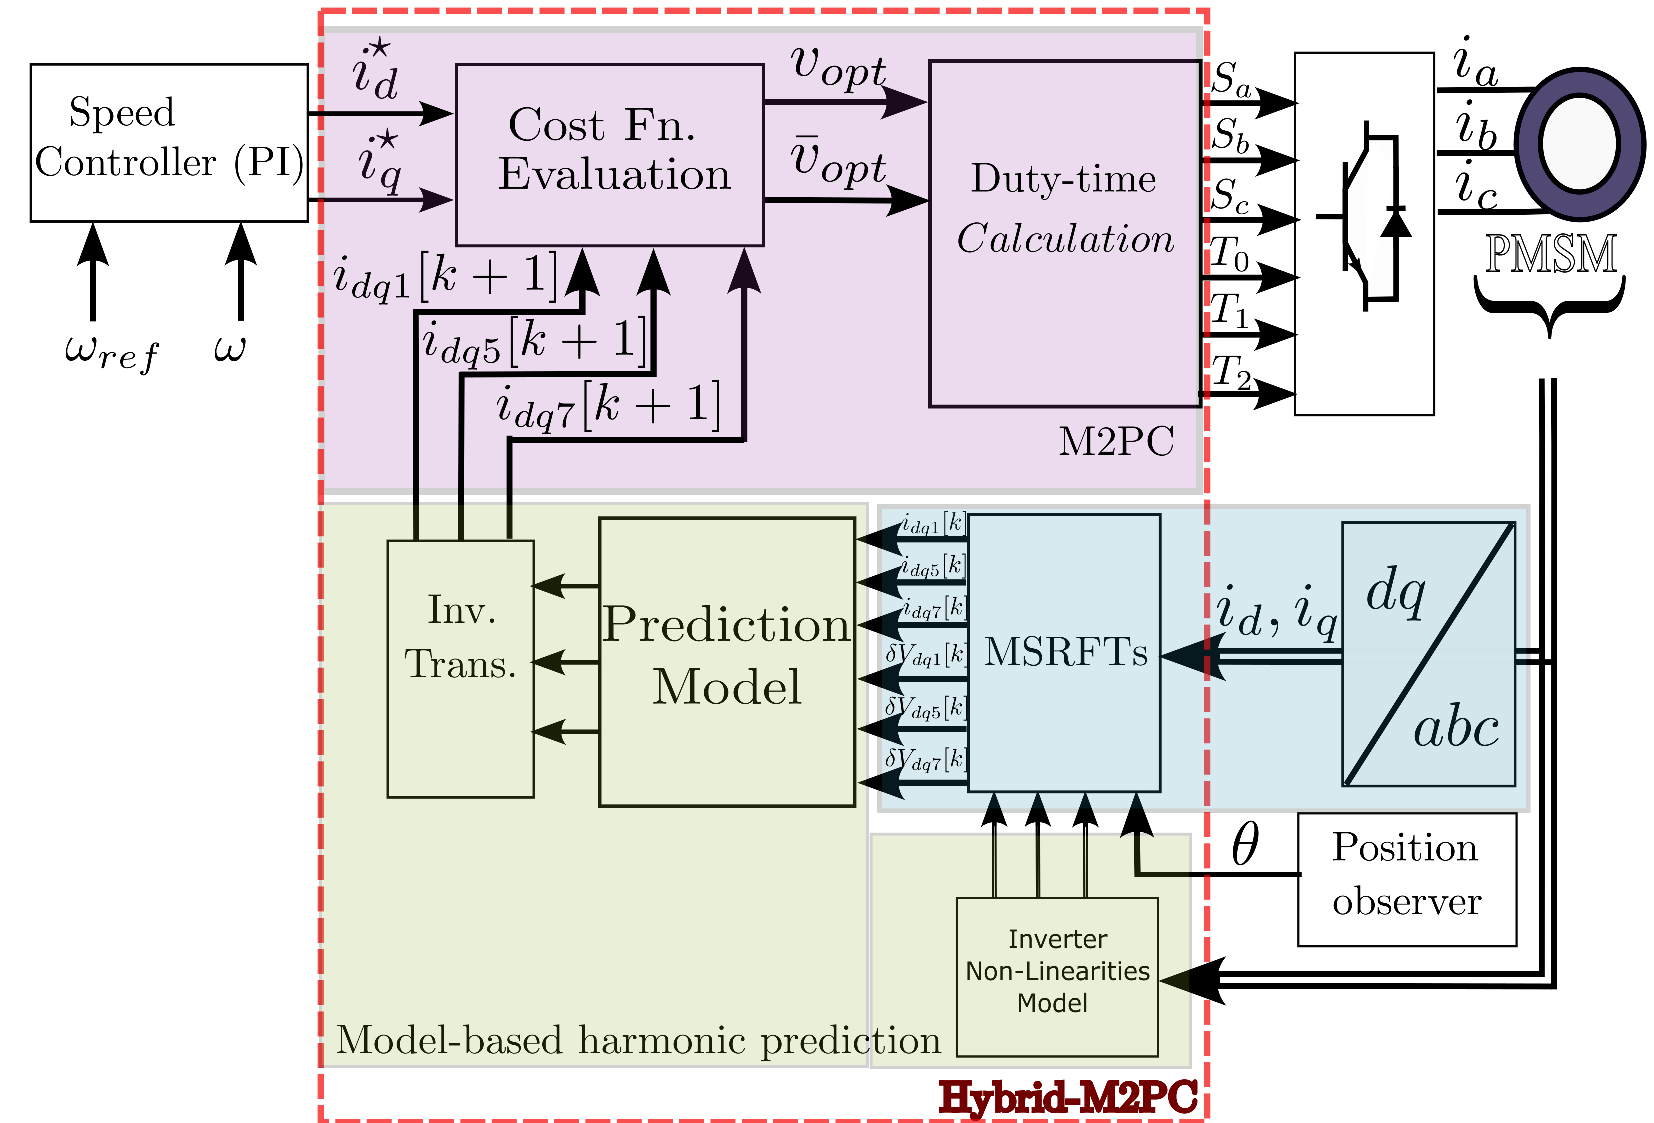
\includegraphics[width=\linewidth]{hybrid_MPC_updated}
\caption{Proposed Hybrid-MMPC scheme for PMSM drives, combining MMPC approach, and harmonic prediction in multiple synchronous rotating frames }
\label{fig:Proposed_M2PC}
\end{figure}

To realize optimal voltage application within a single sampling period, the control strategy involves selecting two active voltage vectors, \( \mathbf{v}_{\text{opt}} \) and \( \mathbf{v}'_{\text{opt}} \), along with the zero vector \( \mathbf{v}_0 \). The sub-indices 0, 1, and 2 correspond to the zero vector \( \mathbf{v}_0 \), the optimal voltage vector \( \mathbf{v}_{\text{opt}} \), and the second optimal vector \( \mathbf{v}'_{\text{opt}} \), respectively, selected based on minimizing the cost function defined in~\eqref{eq:cost_function_total}. These vectors are time-modulated during the sampling interval such that their weighted average closely approximates the desired voltage, thereby reducing the current tracking error to nearly zero. the following equations clarify this objective;

\begin{align}
\sum_{j=0}^{2} T_j\, i_{d,v_j}[k+1] &= T_s\, i_d^{*} \label{eq:modulated_mpc_constraints_1}\\
\sum_{j=0}^{2} T_j\, i_{q,v_j}[k+1] &= T_s\, i_q^{*} \label{eq:modulated_mpc_constraints_2}
\end{align}
where
\begin{equation}
\sum_{j=0}^{2} T_j = T_s
\label{eq:modulated_mpc_constraints_3}
\end{equation}
Here, equations~\eqref{eq:modulated_mpc_constraints_1}–\eqref{eq:modulated_mpc_constraints_3} define a linear system of equations used to determine the optimal duty times \( T_0, T_1, T_2 \) associated with the selected voltage vectors \( v_j \). These equations ensure that the weighted sum of the resulting currents aligns with the desired current reference \( (i_d^*, i_q^*) \) over one sampling interval \( T_s \), while also satisfying the time constraint on vector modulation. The duty times \( T_0, T_1, T_2 \) can be computed by solving the following linear system:
\begin{equation}
\begin{bmatrix}
i_{d,v_0}[k+1] & i_{d,v_1}[k+1] & i_{d,v_2}[k+1] \\
i_{q,v_0}[k+1] & i_{q,v_1}[k+1]  & i_{q,v_2}[k+1]  \\
1        & 1        & 1
\end{bmatrix}
\begin{bmatrix}
T_0 \\ T_1 \\ T_2
\end{bmatrix}
=
\begin{bmatrix}
T_s i_d^* \\ T_s i_q^* \\ T_s
\end{bmatrix}
\label{eq:duty_time_solution}
\end{equation}

\noindent
Thus, the optimal duty vector is computed as:
\begin{equation}
\begin{bmatrix}
T_0 \\ T_1 \\ T_2
\end{bmatrix}
=
\begin{bmatrix}
i_{d,v_0}[k+1] & i_{d,v_1}[k+1] & i_{d,v_2}[k+1] \\
i_{q,v_0}[k+1] & i_{q,v_1}[k+1]  & i_{q,v_2}[k+1]  \\
1        & 1        & 1
\end{bmatrix}^{-1}
\begin{bmatrix}
T_s i_d^* \\ T_s i_q^* \\ T_s
\end{bmatrix}
\label{eq:duty_time_closed_form}
\end{equation}

\section{Control Algorithm Summary}
% Harmonic Current Prediction and Compensation — plain enumerate (no algorithm packages)

\begin{enumerate}
  \item Measure the phase currents and transform them to the fundamental $d$–$q$ frame.

  \item Obtain the separated components
  $
  \begin{bmatrix} i_{d1}[k]\\ i_{q1}[k]\end{bmatrix},\ 
  \begin{bmatrix} i_{d5}[k]\\ i_{q5}[k]\end{bmatrix}_{\text{5th-frame}},\ 
  \begin{bmatrix} i_{d7}[k]\\ i_{q7}[k]\end{bmatrix}_{\text{7th-frame}}.
  $

  \item Compute the one-step-ahead nominal prediction (fundamental frame):
  \[
  \begin{bmatrix} i_{d1}[k+1]\\ i_{q1}[k+1]\end{bmatrix}
  =
  \left(1-\frac{R T_s}{L}\right)
  \begin{bmatrix} i_{d1}[k]\\ i_{q1}[k]\end{bmatrix}
  + \frac{T_s}{L}\begin{bmatrix} v_d[k]\\ v_q[k]\end{bmatrix}
  + \omega T_s \begin{bmatrix} i_{q1}[k]\\ -\,i_{d1}[k]\end{bmatrix}
  + \frac{\omega T_s}{L}\begin{bmatrix} 0\\ \lambda_m\end{bmatrix}.
  \]

  \item Using the predicted currents from Step 3, compute the nonlinear voltage drop $\delta v_{\mathrm{th}}$ from (\ref{eq:distortion_voltage}).

  \item Form the decomposed voltage-drop components
  $
  \begin{bmatrix}\delta v_{d1}[k]\\ \delta v_{q1}[k]\end{bmatrix},\
  \begin{bmatrix}\delta v_{d5}[k]\\ \delta v_{q5}[k]\end{bmatrix}_{\text{5th-frame}},\
  \begin{bmatrix}\delta v_{d7}[k]\\ \delta v_{q7}[k]\end{bmatrix}_{\text{7th-frame}}.
  $

  \item Predict currents in the 5th and 7th frames using (\ref{eq:id5_predict}) and (\ref{eq:id7_predict}).

  \item Transform the predicted harmonic-frame currents back to the fundamental frame:
  \[
  \begin{bmatrix} i_{d5}[k+1]\\ i_{q5}[k+1] \end{bmatrix}
  = \left(T_{dq1}^{dq5}\right)^{-1}
    \begin{bmatrix} i_{d5h}[k+1]\\ i_{q5h}[k+1]\end{bmatrix},
  \qquad
  \begin{bmatrix} i_{d7}[k+1]\\ i_{q7}[k+1] \end{bmatrix}
  = \left(T_{dq1}^{dq7}\right)^{-1}
    \begin{bmatrix} i_{d7h}[k+1]\\ i_{q7h}[k+1]\end{bmatrix}.
  \]

  \item Evaluate the cost function $J(v_i)$ using the predicted currents.

  \item Store the pair $(J, v_i)$ for later selection.

  \item Repeat Steps 1–9 for $i=0,\ldots,7$.

  \item Select the optimal and sub-optimal switching vectors $(v_1, v_2)$ that yield the minimum $J$.

  \item Compute the duty times $T_0, T_1, T_2$ using (\ref{eq:duty_time_closed_form}).
\end{enumerate}
\section{Simulation Modeling}
This section validates the complete drive model and controllers through a focused suite of studies: (i) steady-state operation to verify ripple, losses, and harmonic content; (ii) low-speed operation to probe back-EMF limits and non-idealities; (iii)  dynamic performance under speed/current steps; (iv) parameter variation to gauge robustness against model mismatch; and (v) load variation to assess torque disturbance rejection.
\subsection{Steady State Operation}
At 1000 rpm with dead time and device drops enabled, the MMPC augmented with harmonic extraction sustains tight regulation and further reduces ripple relative to the basic MMPC. At low load (10\% rated torque, \(0.3~\mathrm{N\,m}\)) the phase-current THD drops to 6.5\% (vs.\ \(\sim\)8\% basic), see Fig.~\ref{fig:M2PCNL_HE_1000rpm_low}; at medium load (50\% rated torque, \(1.75~\mathrm{N\,m}\)) it falls to 0.8\% (vs.\ \(\sim\)2\% basic), see Fig.~\ref{fig:M2PCNL_HE_1000rpm_med}. These improvements—about \(1.5\) and \(1.2\) percentage points, respectively—reflect extraction/cancellation of the dominant low-order odd harmonics injected by non-ideal switching, while preserving fixed-frequency SVM actuation and excellent steady-state speed regulation.
% Requires in preamble:
% \usepackage{graphicx}
% \usepackage{subcaption}

\begin{figure}[H]
  \centering
  % --- (a) Low load with harmonic extraction ---
  \begin{subfigure}{0.485\textwidth}
    \centering
    % Replace with your exported plot/image
    
\includegraphics[width=\linewidth]{MPCMidSpeedLowLoadSteadyState}
    \caption{Low load: \(T=0.3~\mathrm{N\,m}\). THD \(=6.5\%\) (vs.\ \(8\%\) basic).}
    \label{fig:M2PCNL_HE_1000rpm_low}
  \end{subfigure}\hfill
  % --- (b) Medium load with harmonic extraction ---
  \begin{subfigure}{0.485\textwidth}
    \centering
    % Replace with your exported plot/image
    
\includegraphics[width=\linewidth]{MPCMidSpeedMidLoadSteadyState}
    \caption{Medium load: \(T=1.75~\mathrm{N\,m}\). THD \(=0.8\%\) (vs.\ \(2\%\) basic).}
    \label{fig:M2PCNL_HE_1000rpm_med}
  \end{subfigure}

  \caption{MMPC with harmonic extraction at 50\% rated speed (1000 rpm) under inverter non-linearities (dead time, device drops). Each panel shows \(i_{dq}\), phase currents, and THD.}
  \label{fig:M2PCNL_HE_1000rpm}
\end{figure}


\subsection{Low Speed Operation}

\begin{figure}[H]
  \centering

  % --- Row 1: 5% rated speed (100 rpm) ---
  \begin{subfigure}{0.4\textwidth}
    \centering
    % Replace with your exported plot/image
    
\includegraphics[width=\linewidth]{./MPCSteadyStateLowLoad100Rpm}
    \caption{5\% speed (100 rpm), low load \(T=0.3~\mathrm{N\,m}\); THD \(=2.8\%\).}
    \label{fig:M2PCNL_HE_100rpm_low}
  \end{subfigure}\hfill
  \begin{subfigure}{0.4\textwidth}
    \centering
    % Replace with your exported plot/image
    
\includegraphics[width=\linewidth]{./MPCSteadyStateHighLoad100Rpm}
    \caption{5\% speed (100 rpm), rated load \(T=3.5~\mathrm{N\,m}\); THD \(=0.8\%\).}
    \label{fig:M2PCNL_HE_100rpm_high}
  \end{subfigure}

  \vspace{0.6em}

  % --- Row 2: 10% rated speed (200 rpm) ---
  \begin{subfigure}{0.4\textwidth}
    \centering
    % Replace with your exported plot/image
    
\includegraphics[width=\linewidth]{./MPCSteadyStateLowLoad200Rpm}
    \caption{10\% speed (200 rpm), low load \(T=0.5~\mathrm{N\,m}\); THD \(=2.9\%\).}
    \label{fig:M2PCNL_HE_200rpm_low}
  \end{subfigure}\hfill
  \begin{subfigure}{0.4\textwidth}
    \centering
    % Replace with your exported plot/image
    
\includegraphics[width=\linewidth]{./MPCSteadyStateHighLoad200Rpm}
    \caption{10\% speed (200 rpm), rated load \(T=3.5~\mathrm{N\,m}\); THD \(=0.6\%\).}
    \label{fig:M2PCNL_HE_200rpm_high}
  \end{subfigure}

  \caption{Proposed MMPC-HE at low speeds under inverter non-linearities (dead time, device drops). Each panel shows \(i_{dq}\), phase currents, and THD.}
  \label{fig:M2PCNL_HE_low_speeds}
\end{figure}
With dead time and device drops enabled, the MMPC with harmonic extraction maintains stable sensorless operation and markedly reduces distortion at very low speeds. At 5\% rated (100~rpm), the phase-current THD is 2.8\% at low load (\(0.3~\mathrm{N\,m}\); see Fig.~\ref{fig:M2PCNL_HE_100rpm_low}) versus \(\sim\)6.9\% for the MMPC, and 0.8\% at rated load (\(3.5~\mathrm{N\,m}\); see Fig.~\ref{fig:M2PCNL_HE_100rpm_high}) versus \(\sim\)1.1\%. At 10\% rated (200~rpm), THD is 2.9\% at low load (\(0.5~\mathrm{N\,m}\); see Fig.~\ref{fig:M2PCNL_HE_200rpm_low}) compared with \(\sim\)6.6\% for the basic scheme, and 0.6\% at rated load (\(3.5~\mathrm{N\,m}\); see Fig.~\ref{fig:M2PCNL_HE_200rpm_high}) compared with \(\sim\)1.1\%. These gains arise from extracting/cancelling dominant low-order distortion components injected by non-ideal switching while preserving fixed-frequency SVM actuation and accurate one-step prediction, yielding the best low-speed THD among all controllers studied.

\subsection{Dynamic Performance}
With dead time and device drops enabled, the MMPC-HE tracks speed commands across the 10–50\% band (100–1000~rpm) cleanly at both load extremes—low load (\(0.3~\mathrm{N\,m}\); see Fig.~\ref{fig:M2PCNL_HE_Dyn_100to1000_low}) and rated load (\(3.5~\mathrm{N\,m}\); see Fig.~\ref{fig:M2PCNL_HE_Dyn_100to1000_rated}). In all transitions the measured speed follows the reference with overshoot \(\mathbf{<10\%}\) and negligible steady-state error; \(i_q\) steps proportionally, and the phase currents remain notably smooth, yielding lower torque ripple than all other controllers. Importantly, the harmonic–extraction stage—implemented as selective cancellation of low-order distortion in the commanded average voltage—does not alter the closed-loop dynamics: rise/settling times and damping are essentially unchanged from the baseline MMPC.
% Requires in preamble:
% \usepackage{graphicx}
% \usepackage{subcaption}

\begin{figure}[H]
  \centering
  % --- (a) Low load ---
  \begin{subfigure}{0.485\textwidth}
    \centering
    % Replace with your exported plot/image
    
\includegraphics[width=\linewidth]{MPCDynamicResponseLowLoad}
    \caption{Low load: \(T=0.3~\mathrm{N\,m}\). Overshoot \(<10\%\); smooth \(i_q\)/phase currents; very low torque ripple.}
    \label{fig:M2PCNL_HE_Dyn_100to1000_low}
  \end{subfigure}\hfill
  % --- (b) Rated load ---
  \begin{subfigure}{0.485\textwidth}
    \centering
    % Replace with your exported plot/image
    
\includegraphics[width=\linewidth]{MPCDynamicResponseHighLoad}
    \caption{Rated load: \(T=3.5~\mathrm{N\,m}\). Overshoot \(<10\%\); damping and settling comparable to baseline MPC.}
    \label{fig:M2PCNL_HE_Dyn_100to1000_rated}
  \end{subfigure}

  \caption{Dynamic performance of MMPC-HE under inverter non-linearities
  (dead time, device drops) for speed changes within the \(10\%\!\to\!50\%\) rated band (100–1000 rpm). Each panel shows
  command vs.\ speed, \(i_q\), and phase currents.}
  \label{fig:M2PCNL_HE_Dyn_100to1000}
\end{figure}

\subsection{Parameter Variation}
At 5\% rated speed (100~rpm) with dead time and device drops enabled, the proposed controller was stressed with a biased prediction model (\(R_s{+}25\%\), \(L_{d,q}{-}25\%\)). As shown in Fig.~\ref{fig:M2PCNL_HE_ParamVariation}, the phase-current THD is 4.6\%, notably lower than the 8.7\% obtained by the \emph{basic} MMPC under the same bias (cf. Fig.~\ref{fig:M2PCNL_ParamVariation}). The fixed-frequency SVM and per-sample voltage optimization preserve the closed-loop cutoff, but the harmonic-extraction stage is model-referenced; the parameter bias shifts the phase/amplitude of the dominant low-order distortion, so the template is imperfect and cancellation is incomplete—hence reduced (but nonzero) residual harmonics.

% Requires in preamble:
% \usepackage{graphicx}

\begin{figure}[h]
  \centering
  % Replace with your exported composite plot (e.g., speed, dq currents, phase currents, THD)
  
\includegraphics[width=0.7\linewidth]{MPCParameterVariation}
  \caption{Proposed MMPC-HE under parameter variation
  at 5\% rated speed (100 rpm) with inverter non-linearities (dead time, device drops).
  The prediction model is biased with \(R_s{+}25\%\) and \(L_{d,q}{-}25\%\).
  The composite plot reports \(d\)- and \(q\)-axis currents, phase currents, and the THD result.}
  \label{fig:M2PCNL_HE_ParamVariation}
\end{figure}

\subsection{Load Variation}
With dead time and device drops enabled, the motor was held at 1000 rpm while the load torque stepped from 10\% to 100\% of rated in 20\% increments. As shown in Fig.~\ref{fig:M2PCNL_HE_LoadVariation}, the proposed MMPC with harmonic extraction maintains the commanded speed without droop; \(i_q\) increases in clean, proportional steps, and the phase currents remain smooth. Transient metrics—rise time, settling, and damping—are essentially unchanged relative to the baseline MMPC (cf. Fig.~\ref{fig:M2PCNL_LoadVariation}), confirming that the harmonic-extraction stage does not penalize dynamics while preserving (and slightly improving) ripple performance under load changes.

% Requires in preamble:
% \usepackage{graphicx}

\begin{figure}[H]
  \centering
  % Replace with your exported composite plot:
  % (left) speed response, (middle) q-axis current, (right) phase currents
  
\includegraphics[width=0.6\linewidth]{MPCLoadVariation}
  \caption{Proposed MMPC-HE under load variation at 50\% rated speed
  (1000 rpm) with inverter non-linearities (dead time, device drops). The composite figure shows motor speed,
  \(i_q\), and phase currents during torque steps from 10\% to 100\% of rated in 20\% increments.}
  \label{fig:M2PCNL_HE_LoadVariation}
\end{figure}

\section{Experimental Validation}
This section presents the experimental validation of the proposed (MMPC-HE) for mitigating inverter non-linearities in a motor drive system. The experiments assess steady-state and dynamic performance under low-load conditions at a low speed and a higher speed. The MMPC-HE is compared against (MMPC), and a conventional proportional-integral (PI) controller at the higher speed, as the PI controller was unstable at the low speed due to its sensitivity to non-linearities. Performance is evaluated using phase current waveforms, d-q axis currents ($i_d$ and $i_q$), and total harmonic distortion (THD) to quantify harmonic suppression and control accuracy.

The experiments were conducted on a \SI{1}{kW} PMSM test bench, powered by a three-phase voltage source inverter (VSI) operating at a switching frequency of \SI{10}{kHz}. A generator was coupled to the motor to apply controlled load conditions, emphasizing inverter-induced non-linearities. The control algorithms were implemented on a Texas Instruments C2000 digital signal processor (DSP) with a control cycle update of \SI{100}{\micro\second}. Phase current measurements were obtained using two high-precision Hall-effect sensors.

Performance metrics include phase current waveforms, d-q axis currents ($i_d$ and $i_q$), and total harmonic distortion (THD).
\subsection{Steady-State Performance}
% Outlining the steady-state test design and evaluation metrics
Steady-state tests were conducted at the low and higher speeds to evaluate harmonic suppression and control accuracy at low loads, 10\% of the rated load. At the low speed, MMPC-HE and MMPC were compared, while at the higher speed, the PI controller was included as a baseline. The evaluation metrics included phase current waveforms to visually inspect harmonic distortions, d-q axis currents to assess control accuracy in the synchronous reference frame, and THD, defined as the percentage ratio of harmonic amplitudes to the fundamental component. 

% Presenting and analyzing steady-state results
The steady-state results are summarized in Table~\ref{tab:steady_state_results} and illustrated in Figures~\ref{fig:steady_state_100rpm}and~\ref{fig:steady_state_200rpm}. At the low speed, MMPC-HE exhibited significantly lower THD compared to MMPC, indicating effective harmonic suppression. At the higher speed, MMPC-HE outperformed both MMPC and the PI controller in THD reduction. Phase current waveforms for MMPC-HE showed smoother profiles with minimal distortions, and d-q axis currents displayed reduced oscillations, confirming superior tracking accuracy. The THD improvement of MMPC-HE was statistically significant, MMPC-HE demonstrated enhanced harmonic suppression under similar conditions.

\begin{table}[h]
\centering
\caption{Steady-State THD Comparison at Low Load}
\label{tab:steady_state_results}
\begin{tabular}{l c c}
\hline
Method & THD (100 RPM) & THD (200 RPM) \\
\hline
PI Controller & -- & 12.3\% \\
MMPC & 5.2\% & 3.1\% \\
MMPC-HE (Proposed) & 4.2\% & 2.3\% \\
\hline
\end{tabular}
\end{table}

\begin{figure}[H]
\centering
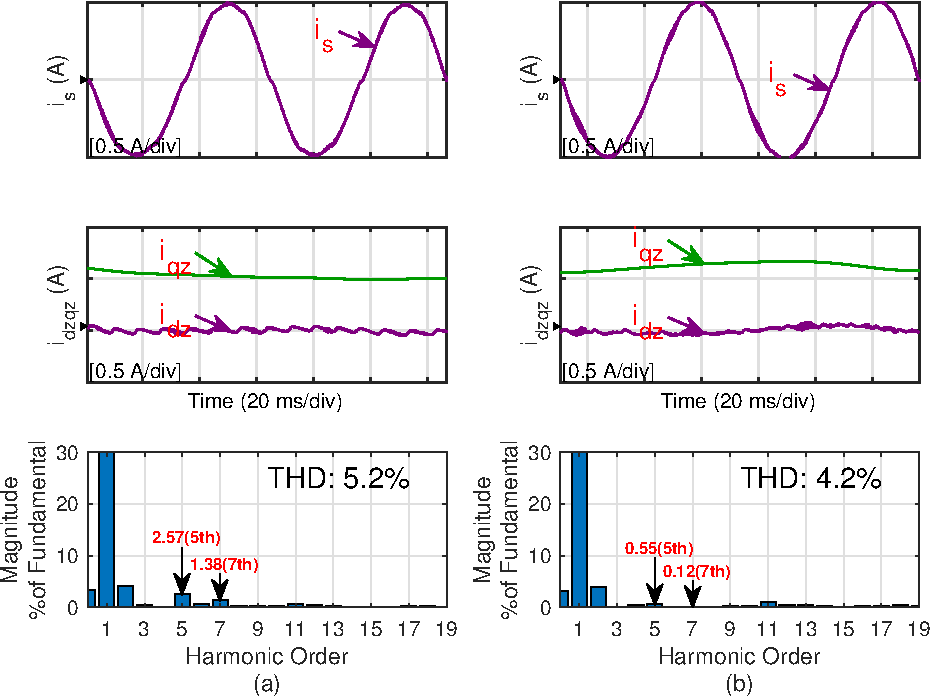
\includegraphics[width=0.8\textwidth]{./SteadyState100Rpm.pdf}
\caption{Experimental results of stator currents, $dz-qz$ axes currents, THD in low-speed (100 RPM) light load condition. (a) MMPC, (b) MMPC-HE.}
\label{fig:steady_state_100rpm}
\end{figure}

\begin{figure}
\centering
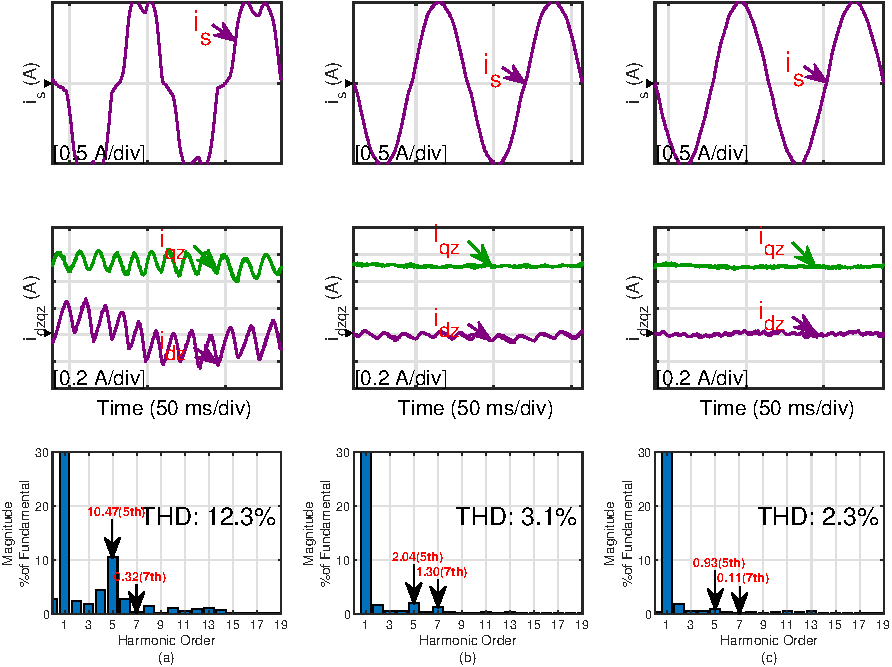
\includegraphics[width=0.8\textwidth]{./SteadyState200Rpm.pdf}
\caption{Experimental results of stator currents, $dz-qz$ axes currents, THD in low-speed (200 RPM) light load condition. (a) PI-Controller (b) MMPC, (c) MMPC-HE.}
\label{fig:steady_state_200rpm}
\end{figure}

\begin{figure}[H]
\centering
\includegraphics[width=8cm]{./hardware_setup}
\caption{Hardware setup}
\label{fig:hardware_setup}
\end{figure}

\subsection{Dynamic Response}
Dynamic response tests assessed the transient performance of the control methods under two speed step conditions. The first test evaluated MMPC-HE alone for a speed step from \SI{100}{rpm} to \SI{500}{rpm} to assess its transient response at higher speeds. The second test evaluated MMPC-HE, MMPC, and the PI controller for a speed step from \SI{500}{rpm} to \SI{100}{rpm} to compare their performance at lower speeds. The metrics included speed response, defined as the time taken for the motor speed to stabilize within a small percentage of the target speed, overshoot in the quadrature-axis current ($i_q$), and stator current waveforms to assess transient harmonic content.

The dynamic response results are presented in Figures~\ref{fig:DynamicHE_response}, and \ref{fig:DynamicAll_response}. For the speed step from \SI{100}{rpm} to \SI{500}{rpm}, MMPC-HE exhibited rapid speed response, minimal $i_q$ overshoot, and stator current waveforms with low harmonic distortion, demonstrating robust transient performance. For the speed step from \SI{500}{rpm} to \SI{100}{rpm}, MMPC-HE achieved a speed response comparable to MMPC-NHE but with significantly reduced $i_q$ undershoot, indicating stable control and rapid response unaffected by the harmonic extraction and elimination correction factor. while the PI controller exhibited an unstable response due to its inability to mitigate non-linearities at low speeds, resulting in pronounced stator current distortions.

\begin{figure}[H]
\centering
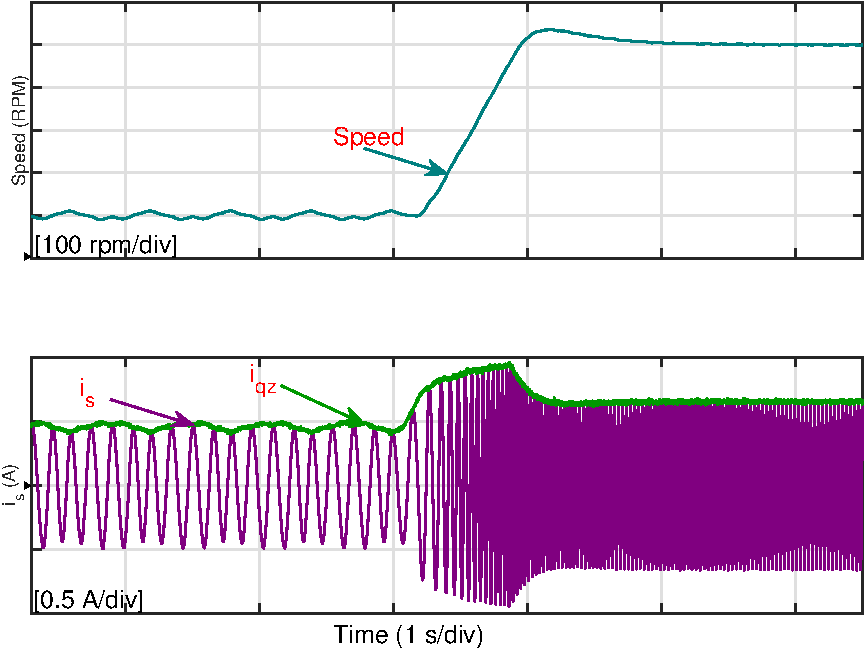
\includegraphics[width=0.6\textwidth]{./DynamicResponseHE.pdf}
\caption{Experimental results of stator currents, $qz$ axis current, and the speed response.}
\label{fig:DynamicHE_response}
\end{figure}

\begin{figure}[H]
\centering
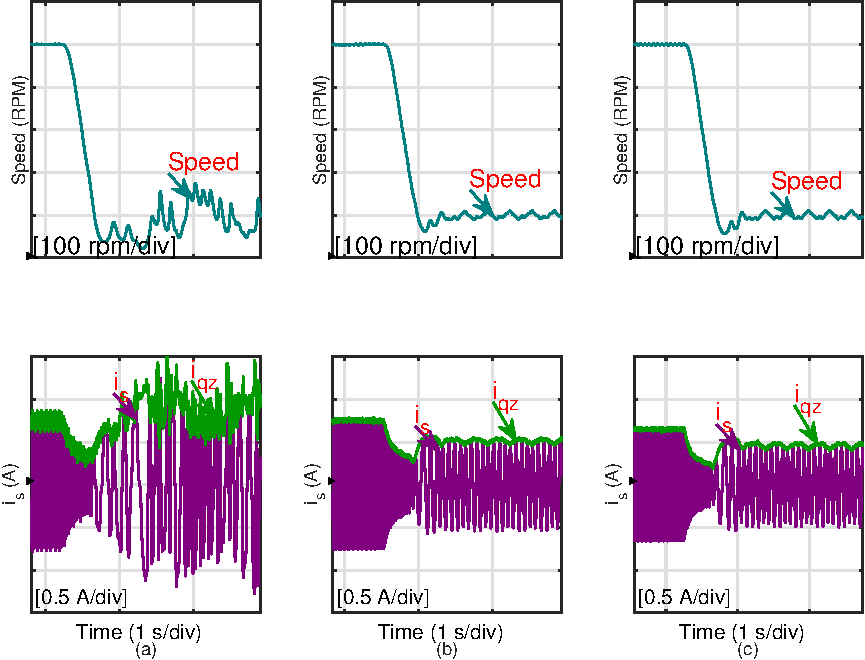
\includegraphics[width=0.6\textwidth]{./DynamicResponseAll.pdf}
\caption{Experimental results of stator currents, $qz$ axis current, and the speed response. (a) PI-Controller (b) MMPC, (c) MMPC-HE.}
\label{fig:DynamicAll_response}
\end{figure}


\subsection{Parameter Variation}
To evaluate the robustness of the proposed controller, a motor parameter variation test was conducted. In this test, key parameters of the permanent magnet synchronous motor (PMSM)—such as stator resistance, and inductance—were intentionally varied within a predefined range to emulate real-world operating conditions, including temperature fluctuations, aging effects, and manufacturing tolerances. The controller’s performance was assessed under these parameter deviations by monitoring current regulation, and overall stability. This procedure allowed for quantifying the sensitivity of the control algorithm to parameter uncertainties and verifying its capability to maintain reliable operation despite motor model mismatches.

The results of the motor parameter variation test, illustrated in Figure \ref{fig:ParameterVariation}, highlight the superior performance of the proposed hybrid modulated model predictive current controller in terms of current quality. When subjected to parameter deviations, the conventional PI current controller exhibited a significant degradation in performance, with the total harmonic distortion (THD) increasing by approximately 7\%. In comparison, the modulated model predictive current controller demonstrated improved robustness, showing only a 0.6\% increase in THD under the same conditions. The proposed hybrid approach achieved the best performance, limiting the THD increase to just 0.2\%, thereby confirming its enhanced capability to handle parameter variations while maintaining high-quality current waveforms

\begin{figure}[H]
\centering

\includegraphics[width=0.6\textwidth]{./ParameterVariation.pdf}
\caption{Experimental results of stator currents, $dz-qz$ axes currents, THD in low-speed (200 RPM) light load condition with motor parameters Variation. (a) PI-Controller (b) MMPC, (c) MMPC-HE.}
\label{fig:ParameterVariation}
\end{figure}

\subsection{CPU Load Consumption}
% Outlining the CPU load test design and evaluation metrics
CPU load consumption tests were conducted to evaluate the computational burden of the control methods, particularly due to the extensive use of sine and cosine operations in MMPC-HE. The tests measured the execution time of each control algorithm on the C2000 DSP under steady-state conditions at the low and higher speeds. The evaluation metric was the percentage of the \SI{100}{\micro\second} control cycle consumed by the algorithm, reflecting the computational load relative to the available processing time.

% Presenting and analyzing CPU load consumption results
The CPU load consumption results are summarized in Table~\ref{tab:cpu_load_results}. At both the low and higher steady state speeds, MMPC-HE exhibited a higher computational load compared to MMPC and the PI controller, attributed to the additional sine and cosine operations required for harmonic extraction and elimination. However, the execution time of MMPC-HE remained within the \SI{100}{\micro\second} control cycle, indicating feasibility for real-time implementation on the C2000 DSP. In contrast, MMPC and the PI controller required less computational time, with the PI controller showing the lowest CPU load due to its simpler control structure. These results highlight a trade-off between the enhanced harmonic suppression of MMPC-HE and its increased computational demand, which warrants further optimization in future work.

\begin{table}[h]
\centering
\caption{CPU Load Consumption Comparison}
\label{tab:cpu_load_results}
\begin{tabular}{l c}
\hline
Method & CPU Load (\%) \\
\hline
PI Controller & 3.5  \\
MMPC & 34\\
MMPC-HE (Proposed) & 45 \\
\hline
\end{tabular}
\end{table}

\begin{figure}[htbp]
    \centering
    \begin{minipage}[b]{0.3\textwidth}
        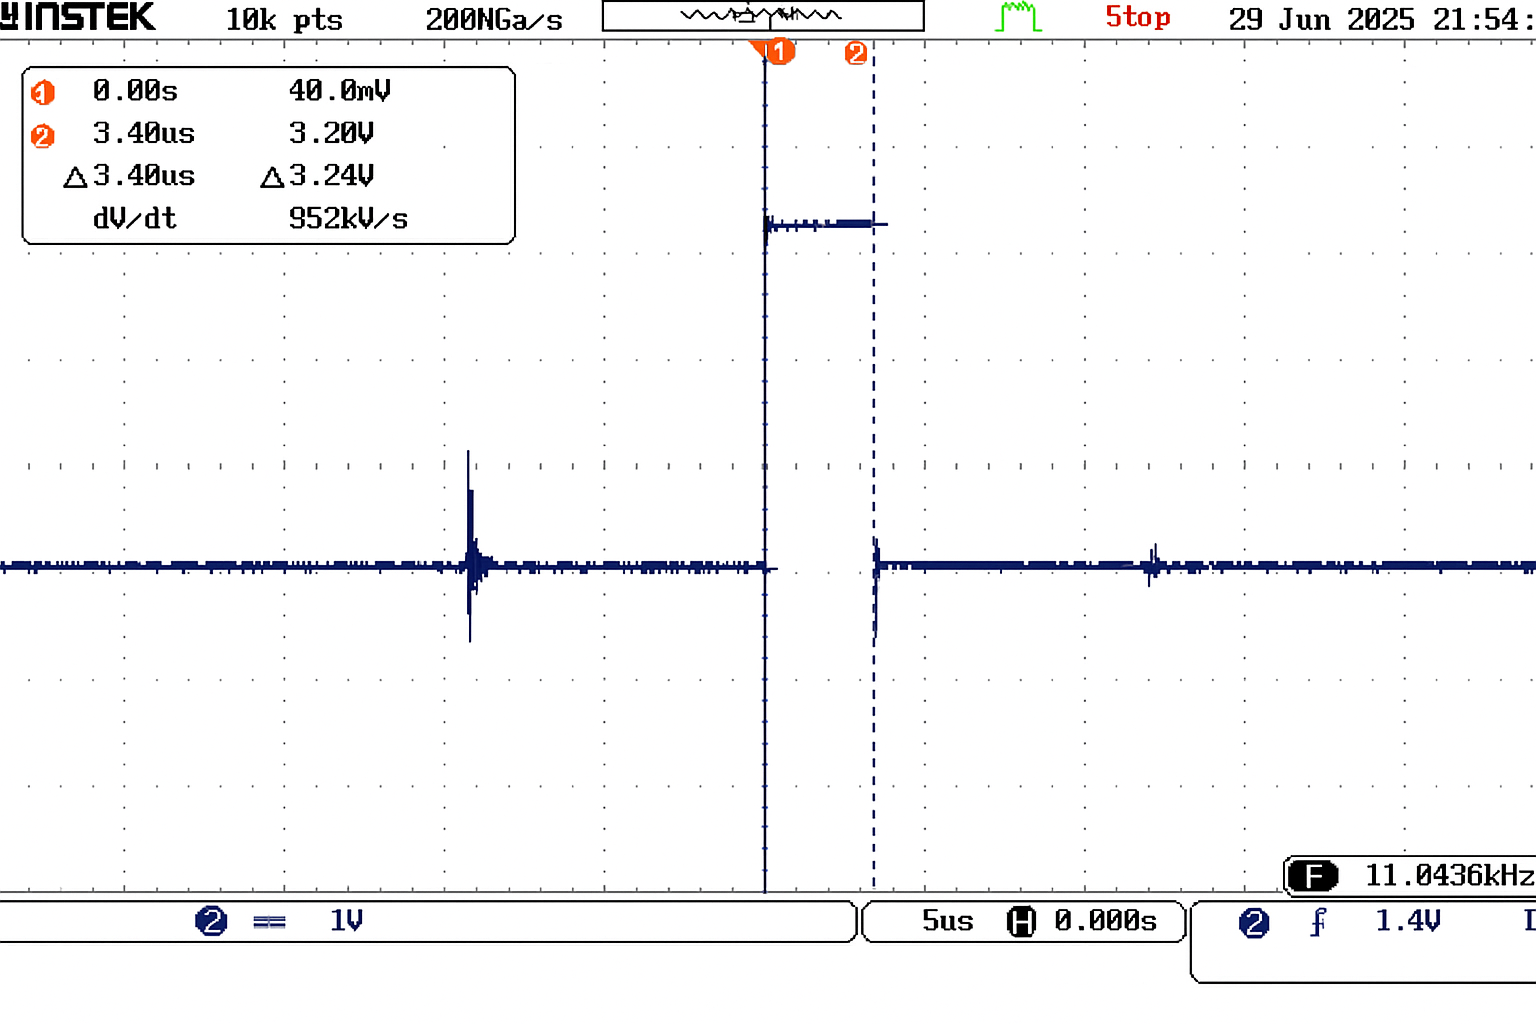
\includegraphics[width=\textwidth]{./CPU_Load_PI}
    \end{minipage}
    \hfill
    \begin{minipage}[b]{0.3\textwidth}
        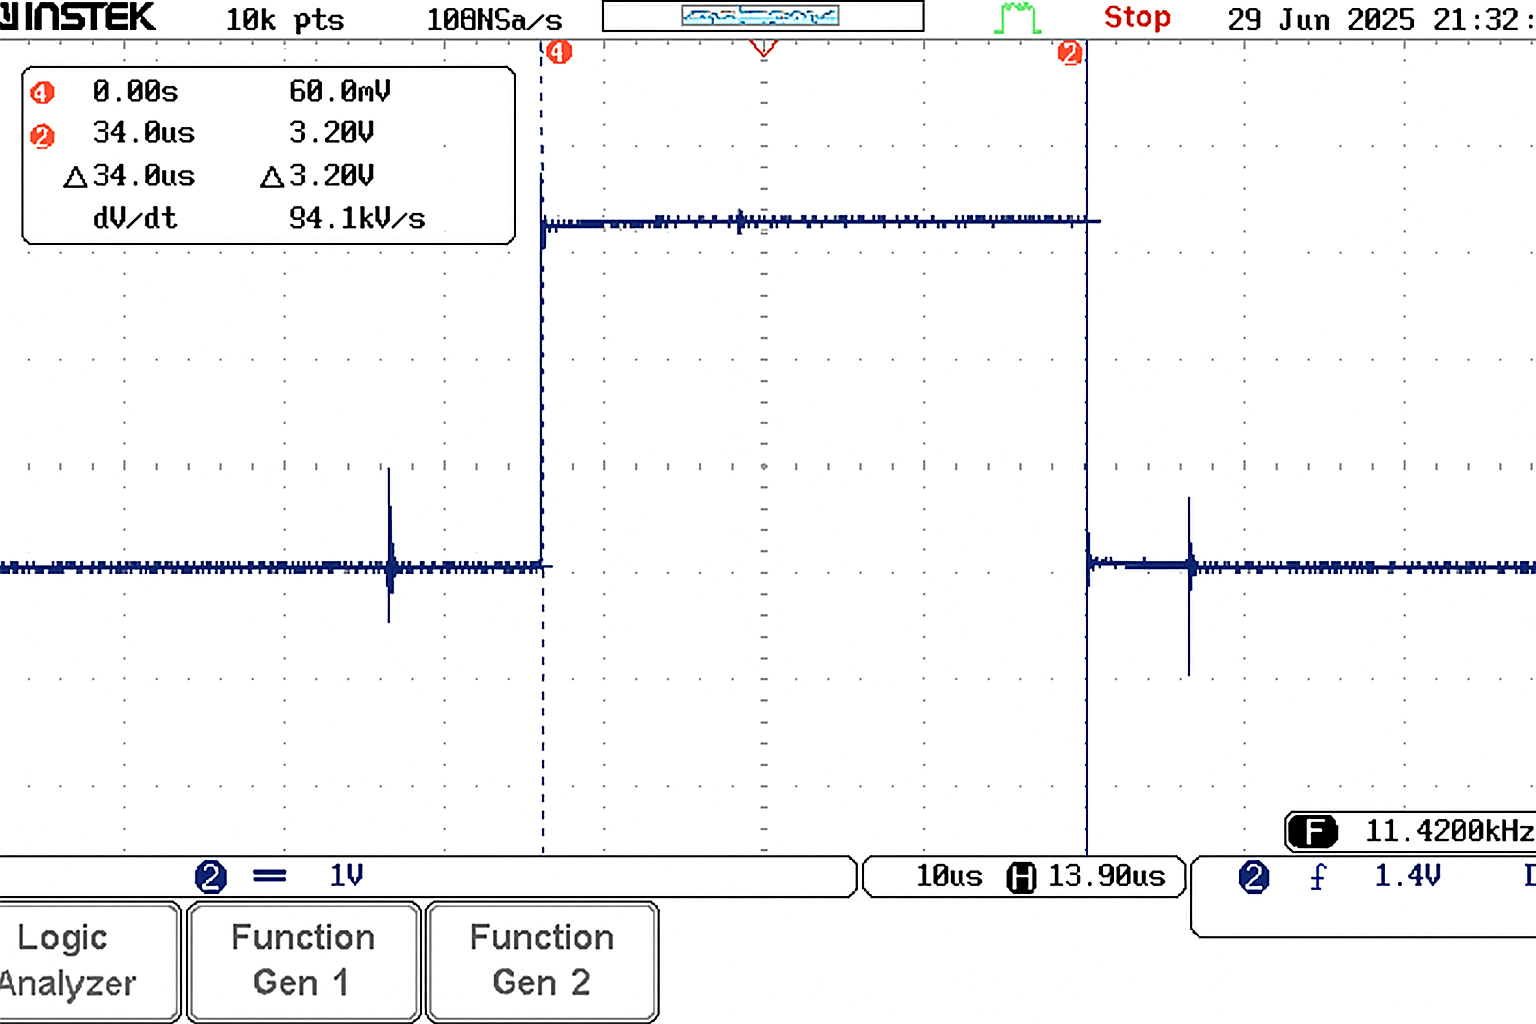
\includegraphics[width=\textwidth]{./CPU_Load_MPC_NHE}
    \end{minipage}
    \hfill
    \begin{minipage}[b]{0.3\textwidth}
        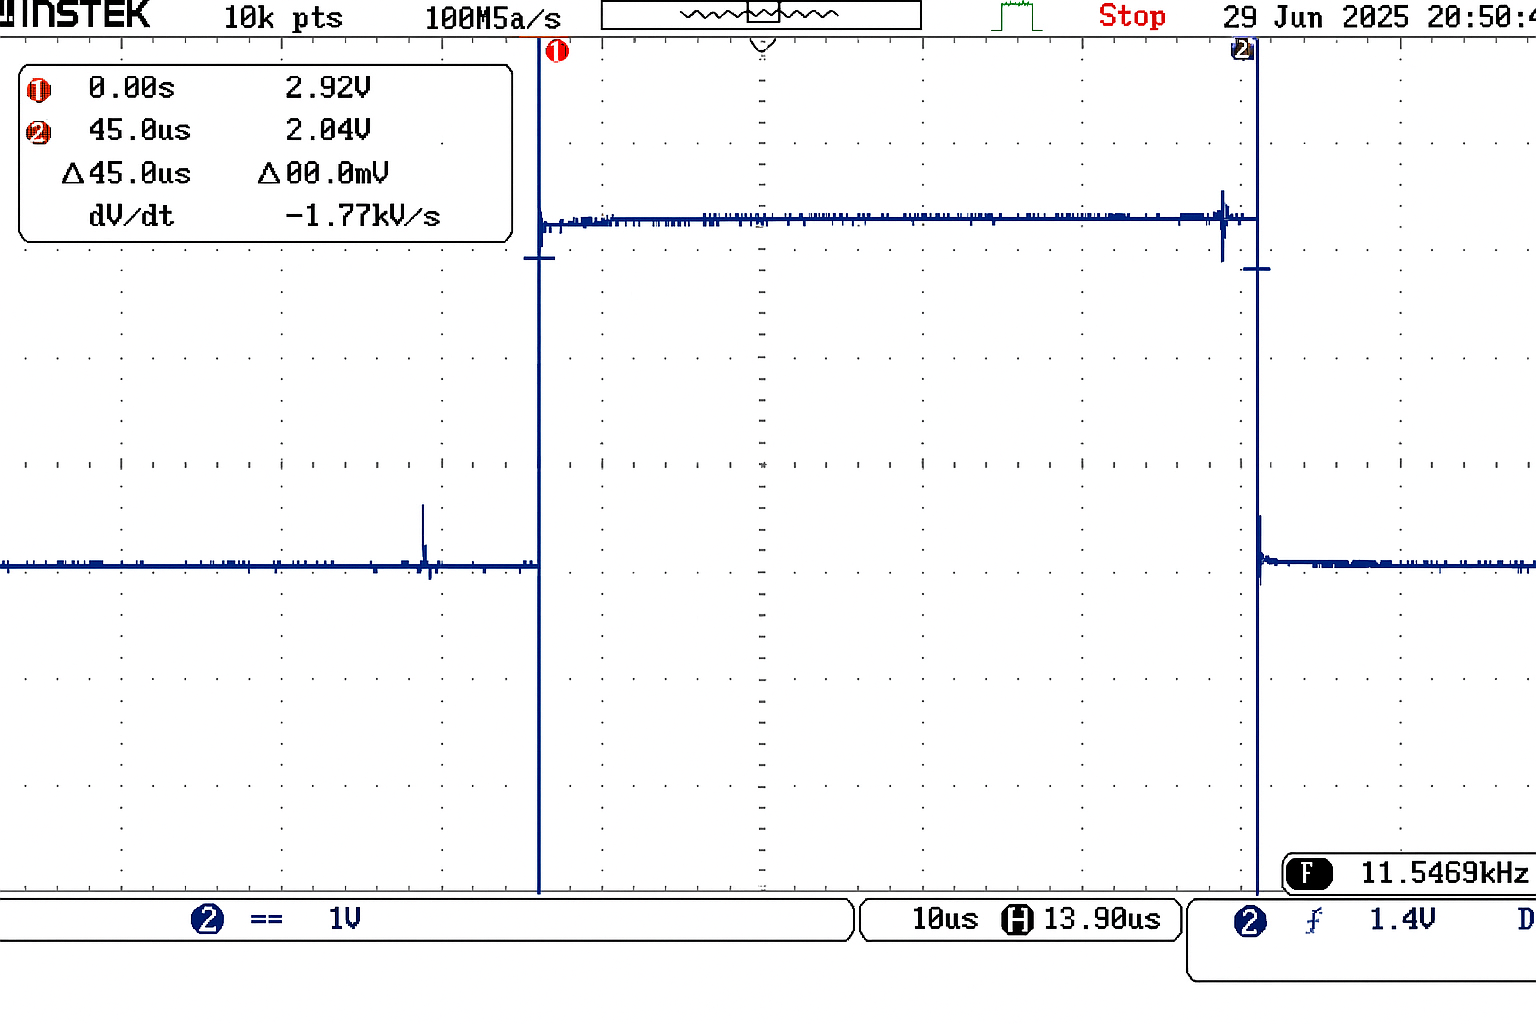
\includegraphics[width=\textwidth]{./CPU_Load_MPC_HE}
    \end{minipage}
    \caption{Experimental results for each controller execution time (a) PI-Controller (b) MMPC, (c) MMPC-HE.}
    \label{fig:minipage_example}
\end{figure}

\chapter{Conclusion and Future Work} \label{chap:conclusion}
\let\cleardoublepage\clearpage
\label{ch:conclusion}

\section*{Summary of the thesis}
This thesis set out to mitigate inverter non\-linearities in PMSM drives using MMPC current control while preserving fixed switching frequency and sensorless operation at low speed. The work progressed from first principles to system-level validation: (i) a physics-based PMSM model was derived from the three-phase $(a,b,c)$ variables to the $dq$ frame, with torque and power relations, (ii) a sensorless pipeline was built around a SMO and a two-stage adaptive low-pass filter whose cut-off tracks electrical speed to guarantee $\approx90^\circ$ net phase at the fundamental, (iii) speed and current PI controllers were designed in series form via explicit plant-pole cancellation, yielding transparent bandwidth targets, (iv) forward-Euler discrete models were adopted for prediction, (v) three control baselines were implemented—PI–FOC, (FCS–MPC), and a MMPC that optimizes a continuous average voltage and realizes it by SVM—and (vi) a proposed enhancement introduced harmonic extraction to cancel dominant low-order distortion in the commanded average voltage. Practical parameter identification was carried out and reused throughout: $R_{\mathrm{LL}}=2.67~\Omega$ (lead-inclusive), $L_d=2.87~\mathrm{mH}$, $L_q=2.58~\mathrm{mH}$, $\lambda=0.1227~\mathrm{Wb}$, $J=0.00636~\mathrm{kg\,m^2}$, and $B=0.004775~\mathrm{N\,m\,s/rad}$.

\section*{Key quantitative findings}
Under ideal conditions, PI–FOC delivers clean steady state at mid-speed (e.g., $\approx0.8\%$ THD at $1000~\mathrm{rpm}$) and well-damped dynamics; FCS–MPC exhibits the expected staircase-voltage penalty (e.g., $\approx8\%$ THD at $1000~\mathrm{rpm}$; up to $32\%$ at $100~\mathrm{rpm}$ and low load), while MMPC achieves low ripple (down to $0.4\%$ THD at $100~\mathrm{rpm}$, rated load) with overshoot $<10\%$. Parameter-mismatch tests highlighted model sensitivity: MPC-FCS degraded markedly ($32\%\!\to\!41\%$ THD at $100~\mathrm{rpm}$, low load), PI rose slightly ($1.3\%\!\to\!1.7\%$), and MMPC was essentially invariant ($\approx0.3\%$).

With inverter non-linearities (dead time, device drops), PI’s harmonic floor rose sharply at light load and low speed (e.g., $16.4\%$ at $1000~\mathrm{rpm}$ low load; $23.2\%$ at $200~\mathrm{rpm}$ low load) and it became unstable at $100~\mathrm{rpm}$. FCS–MPC stabilized from $200~\mathrm{rpm}$ upward but retained high ripple (e.g., $17\%$ at $1000~\mathrm{rpm}$, $34\%$ at $200~\mathrm{rpm}$ low load) and failed certain step-down transients. In contrast, MMPC preserved fixed switching frequency and delivered much lower THD (e.g., $8\%$ at $1000~\mathrm{rpm}$ low load; $1.1\%$ at $100$–$200~\mathrm{rpm}$ rated load), with overshoot $<10\%$. The MMPC-HE further reduced distortion at the same operating points (e.g., $6.5\%$ and $0.8\%$ THD at $1000~\mathrm{rpm}$ low/medium load) and at very low speeds (e.g., $2.8\%$ at $100~\mathrm{rpm}$ low load; $2.9\%$ at $200~\mathrm{rpm}$ low load). Under the worst $\pm25\%$ $R$–$L$ bias with non-linearities at $100~\mathrm{rpm}$, the proposed scheme still outperformed the basic MMPC (e.g., $4.6\%$ vs.\ $8.7\%$ THD), evidencing robustness even when the harmonic template is imperfect.

\section*{What the comparisons say}
Three clear lessons emerged:
\begin{itemize}
  \item \textbf{Actuation matters:} fixing the switching frequency and optimizing a continuous average voltage (MMPC) is the dominant lever for ripple reduction; single-vector FCS-MPC is intrinsically disadvantaged at low-voltage points, especially with sensorless operation.
  \item \textbf{Model quality matters differently across schemes:} MPC-FCS decisions hinge on one-step predictions for a single vector, so $R$–$L$ errors directly misrank candidates; PI tolerates modest plant shifts but cannot reject additive harmonic bias; MMPC is largely insensitive to moderate $R$–$L$ errors because SVM realizes the optimizer’s average voltage every sample.
  \item \textbf{Structured compensation helps:} MMPC-HE targets the low-order odd components introduced by non-ideal switching, lowering THD further without altering closed-loop dynamics.
\end{itemize}

\section*{Practical design takeaways}
A pragmatic path for PMSM drives that must operate sensorlessly and quietly at low speed is: (i) identify $R_{\mathrm{LL}},L_d,L_q,\lambda,J,B$ with simple lab procedures and reuse them across all controllers; (ii) if a PI baseline is required, design series PI loops by explicit plant-pole cancellation and keep bandwidth moderate; expect limited benefit against additive voltage distortion; (iii) prefer MMPC for low ripple and predictable EMI; and (iv) when non-linearities dominate, add harmonic extraction on the commanded average voltage to shave the remaining low-order content with negligible dynamic cost.

\section*{Limitations}
All dynamic and steady-state results were obtained in simulation. Core non-idealities (dead time, device drops, computation delay) were modeled as effective voltage biases, but additional phenomena—magnetic saturation/cross-saturation, spatial harmonics, temperature drift of $R$ and magnet flux, inverter latency jitter, ADC quantization/latency, and PWM nonlinearity beyond the nominal bias model—were not exhaustively covered. The harmonic-extraction stage relies on a model-referenced template; large parameter drifts or saliency-dependent harmonic phasing can leave residuals.

\section*{Future work}
Immediate extensions include: hardware-in-the-loop and bench validation of MMPC and the harmonic-extraction stage; online adaptation of the harmonic template using measured current spectra; joint estimation of $R$, $L_d$, $L_q$, and $\lambda$ to maintain model fidelity; inclusion of saturation and cross-coupling in the predictor; extension to field-weakening and MTPA; and embedded implementation aspects (fixed-point arithmetic, scheduler co-design with PWM/ADC timing) to preserve the assumed one-sample prediction horizon. Exploring multi-objective MPC that explicitly trades THD, switching loss, and acoustic metrics at runtime is also promising.

\section*{Closing remark}
Overall, the thesis demonstrates that MMPC—particularly with harmonic extraction—offers a practical, robust, and low-ripple route to mitigating inverter non-linearities in sensorless PMSM drives across the operating envelope, improving spectral cleanliness and dynamic behavior beyond PI–FOC and FCS–MPC while keeping the computational footprint modest.








% to change default biblography naming 
\renewcommand\bibname{References} 
%%\bibliography{Thesis}
%%\bibliographystyle{IEEEtran}
%\cleardoublepage
\phantomsection
\addcontentsline{toc}{chapter}{References}
\printbibliography
%
\includepdf[pages={23-27}]{Chapters/FrontPages/CUFEThesisTemplate.pdf}
\end{document}
